% htlatex
\documentclass[12pt,ngerman,a4paper,fullparskip]{report}

%\usepackage[left=2cm,top=3cm,bottom=3cm]{geometry}
\usepackage[utf8]{inputenc}
\usepackage[T1]{fontenc}


\usepackage{booktabs}
\usepackage{babel}
\usepackage{graphicx}
\usepackage{csquotes}
\usepackage{paralist}
\usepackage{xcolor}
\usepackage{xspace}
\usepackage{url}
\usepackage{multicol}
\usepackage{alltt,verbatim}

\newcommand{\tlcurrentyear}{2023}
\newcommand{\AllTeX}{All\TeX}
\newcommand{\TL}{\TeX\ Live\xspace}
\newcommand{\email}[1]{\texttt{#1}}
\newcommand{\acro}[1]{\texttt{#1}}
\newcommand{\cmdname}[1]{\texttt{#1}}
\newcommand{\code}[1]{\texttt{#1}}
\newcommand{\cs}[1]{\texttt{#1}}
\newcommand{\prog}[1]{\texttt{#1}}
\newcommand{\optname}[1]{\texttt{#1}}
\newcommand{\OnCD}[1]{\texttt{#1}}
\newcommand{\file}[1]{\texttt{#1}}
\newcommand{\filename}[1]{\texttt{#1}}
\newcommand{\dirname}[1]{\texttt{#1}}
\newcommand{\pkgname}[1]{\texttt{#1}}
\newcommand{\Webc}[1]{\texttt{#1}}
\newcommand{\envname}[1]{\texttt{#1}}
\newcommand{\TeXXeT}{TeXXeT}
\newcommand{\KPS}{Kpathsea\xspace}
\newcommand{\var}[1]{\texttt{#1}}
\newcommand{\samp}[1]{\texttt{#1}}
\newcommand{\Ucom}[1]{\textbf{\texttt{#1}}}
\newcommand{\bs}{\protect\normalfont\ttfamily\char'134}

\usepackage{fancyvrb}
\DefineVerbatimEnvironment{boxedverbatim}{Verbatim}{fontsize=\footnotesize,frame=single}

\setlength{\parskip}{1em}
\setlength{\parindent}{0pt}


\def\TK{\TeX\ Collection}

\newcommand\ConTeXt{C\kern-.0333emon\-\kern-.0667em\TeX\kern-.0333emt}
\newcommand\MIKTEX{MiK\kern-.025em \TeX}% per www.miktex.org

\def\MP{MetaPost}
\def\MF{MetaFont}
\def\BibTeX{Bib\TeX}

\providecommand*{\CD}{\acro{CD}\xspace}
\providecommand*{\CTAN}{\acro{CTAN}\xspace}
\providecommand*{\DVD}{\acro{DVD}\xspace}
\providecommand*{\GNU}{\acro{GNU}\xspace}
\providecommand*{\HTML}{\acro{HTML}\xspace}
\providecommand*{\ISO}{\acro{ISO}\xspace}
\providecommand*{\MacOSX}{Mac\,\acro{OS\,X}\xspace}
\providecommand*{\macOS}{macOS\xspace}
\providecommand*{\PS}{Post\-Script\xspace}
\providecommand*{\TDS}{\acro{TDS}\xspace}
\providecommand*{\USB}{\acro{USB}\xspace}
\providecommand*{\dvi}{\acro{DVI}\xspace}
\providecommand*{\web}{\acro{WEB}\xspace}
\providecommand*{\eTeX}{e\TeX\xspace}
\providecommand*{\XeTeX}{xe\TeX\xspace}

\DeclareGraphicsExtensions{.png,}

\usepackage{url}

\newcommand{\dante}{DANTE~e.\,V\kern-0.15em.}

%\usepackage{bera}
%\usepackage{hyperref}
%\hypersetup{%
%  colorlinks=true,   % aktiviert farbige Referenzen
%  linkcolor = blue,  % Linkfarbe blau
%  citecolor = blue,  % cite-Farbe blau
%  urlcolor = blue,  % cite-Farbe blau
%  pdfpagemode=UseNone,  % PDF-Viewer startet ohne Inhaltsverzeichnis et.al.
%  pdfstartview=FitH} % PDF-Viewer benutzt beim Start bestimmte Seitenbreite
%
%\hypersetup{%
%  pdftitle={TeX Live Anleitung},%
%  pdfauthor={Uwe Ziegenhagen, ww.uweziegenhagen.de},%
%  pdfsubject={TeX Live },%
%  pdfkeywords={TeX, LaTeX, TeX Live}%
%}
%\usepackage[tocindentauto]{tocstyle}


\newcommand{\href}[2]{#1}
\usepackage{tex4ht}



\begin{document}


\begin{titlepage}

\begin{center}
\vspace*{3cm}

 \Huge Anleitung zur \TL Installation \vspace*{1cm}

\Large Version \tlcurrentyear

\end{center}

\vfill \noindent Karl Berry (Herausgeber) \\
verantwortlich für die deutsche Ausgabe:\\ 
Dr.~Uwe Ziegenhagen, \href{mailto:ziegenhagen@gmail.com}{ziegenhagen@gmail.com} \\
Köln, \today
\end{titlepage}

%\vspace*{5cm}
%\begin{center}
%Die diesjährige \TeX\ Live Distribution ist Sebastian Rahtz und \\ Peter Breitenlohner gewidmet, die leider verstorben sind. 
%\end{center}

\tableofcontents

%\begin{center}
%Diese Ausgabe von  \TeX\ Live ist Staszek Wawrykiewicz gewidmet.
%\end{center}


\listoffigures

%\listoftables


%
%
%\section{Einleitung}\label{sec:intro}
%\subsection{\TL\ und die \TeX-Collection}


\chapter{Einleitung}\label{sec:intro}
\section{\TL und die \TL-Collection}

Diese Anleitung beschreibt das \TL-System an sich, nicht die Arbeit mit \TeX\ bzw. \LaTeX. 

Die {\TL} Distribution enthält \TeX/\LaTeX-Systeme für Linux, verschiedene \acro{UNIX}-Plattformen, {\macOS} und Windows. Sowohl \TL{} als auch die \TK{} sind durch das Engagement vieler Freiwilliger aus vielen \TeX-Vereinen  entstanden. 

Wahrscheinlich haben Sie \TL{} auf einem von zwei Wegen bezogen, entweder per direktem Download von \TL{} oder als Teil der \DVD{} \TK, die von vielen \TeX-Vereinen (u.\,a. \dante) an ihre Mitglieder verschickt werden und in Deutschland über die Fachbuchhandlung Lehmanns (\url{https://www.lob.de})
vertrieben wird. Kapitel~\ref{sec:tl-coll-dists} beschreibt kurz den Inhalt der \TK-\DVD. 



{\TL} enthält lauf"|fähige Versionen von \TeX, \LaTeXe, \ConTeXt, \MF, \MP, {\BibTeX}  und vielen anderen Programmen, sowie eine umfassende Auswahl an Makros, Zeichensätzen und Beschreibungen, die gemäß der Standard"=\TeX"=Verzeichnisstruktur (\TDS) abgelegt sind.

Eine kurze Zusammenfassung der wesentlichen Änderungen der aktuellen \TL-Version gegenüber der Vorgängerversion finden Sie im Kapitel~\ref{sec:tlcurrent} auf Seite~\pageref{sec:tlcurrent}.

\section{Unterstützung verschiedener Betriebssysteme}\label{sec:os-support}

\TL{} enthält direkt ausführbare Programme für viele Unix-basierte Betriebssysteme, insbesondere GNU/Linux und \macOS\ und Cygwin. Selbst wenn für Ihr Unix-System wider Erwarten keine ausführbaren Programme enthalten sind, sollten Sie in der Lage sein, aus den mitgelieferten Programm-Quellen ein funktionierendes \TeX-System zu kompilieren.

Bezüglich Microsoft Windows: Versionen ab Windows~7 werden unterstützt, unter Windows Vista sollte es ebenfalls funktionieren. Auf älteren Windows-Versionen wie Windows~XP oder Windows 2000 lässt sich \TL~ nicht installieren.

Für Windows stellt \TL~ 64-Bit Programme bereit, 32-Bit-Versionen sind nicht mehr enthalten.

\section{Einsatzmöglichkeiten des \TL-Systems der \TeX\ Collection}\label{sec:basic}

Sie können das \TL-System wahlweise von der \DVD oder über das
Internet (\url{https://tug.org/texlive/acquire.html}) installieren.
Der \prog{Net Installer} ist ein kleines Programm,
das die benötigten Teile aus dem Internet nachlädt. Dieser Weg bietet
sich an (eine schnelle und stabile Internetverbindung voraus gesetzt),
wenn Sie kein komplettes \TL{} installieren wollen, sondern Ihr System nur
aus bestimmten Paketen bestehen soll.

Wenn Sie die \DVD{} besitzen (oder das ISO-Image der \DVD{} herunter
geladen haben -- dieses kann auf einigen Systemen sogar direkt als
virtuelles Medium \enquote{gemountet} werden), können Sie \TL{} nach
Wunsch auf Ihrer Festplatte installieren. \TL{} ist nicht direkt von der \DVD{} lauffähig. Sie können aber eine portable Version z.\,B. auf einem USB-Stick installieren, wie in Kapitel~\ref{sec:portable-tl} beschrieben.

Beide Methoden werden in den späteren Abschnitten zur Installation beschrieben, hier daher nur die kurze Zusammenfassung:

\begin{itemize}
\item Für Linux/Unix ist \cmdname{install-tl} das zentrale Installationsskript, unter Windows ist es \cmdname{install-tl-windows}  . Das Installationsskript bietet eine grafische Benutzeroberfläche (GUI) für die Standardinstallation  (den sogenannten \enquote{GUI mode} mit der Option \code{-gui}) sowie einen  Textmodus  mit der Option \code{-gui=text}. Unter \macOS und Windows ist die grafische Benutzeroberfläche Standard. 

\item \TL installiert unter anderem den ">\TL Manager"< mit dem Namen
\prog{tlmgr}. Auch dieser unterstützt Text- und GUI-Mode. Mit diesem
Programm können Sie einerseits Pakete von \TL installieren oder deinstallieren,
andererseits \TL konfigurieren.
\end{itemize}

\section{\TL und Sicherheit}

Nach bestem Wissen und Gewissen kann man sagen, dass die \TeX-Kernprogramme selbst sehr robust sind. Dieses Maß an Robustheit und Sicherheit wird jedoch möglicherweise nicht von allen Programmen erreicht, die Teil von \TL sind. Daher gilt für \TL das, was auch für alle anderen Programme gilt: Vorsicht bei der Verarbeitung von Quellcode, den man nicht genau kennt! Zur Verbesserung der Sicherheit sollte man in diesen Fällen die entsprechenden Dateien in einem neuen Unterverzeichnis oder chroot verarbeiten.

Die Sorge um die Sicherheit gilt vor allem für Microsoft Windows, da Windows-Programme zuerst im aktuellen Verzeichnis suchen, egal wie Pfad-Angaben gesetzt sind. Theoretisch ermöglicht dies eine Reihe von Angriffsszenarien. Viele Sicherheitslücken in Programmen von \TL wurden geschlossen, andere bestehen auch weiterhin, besonders im Umgang mit Drittanbieter-Software. 

Aus diesem Grund empfehlen wir bei der Verarbeitung von unbekanntem Quellcode, auf das Vorhandensein von ausführbaren Dateien im Quellcode-Verzeichnis zu achten. Diese sollten nicht vorhanden sein und erst recht nicht durch die Verarbeitung von \TeX-Quellcode erzeugt worden sein. 

\TeX\ und seine Begleitprogramme können in Dateien schreiben, wenn ein Dokument übersetzt wird. Diese Funktion kann auch missbräuchlich eingesetzt werden. Daher ist bei der Verarbeitung von unbekannten Quellen die Nutzung eines neuen Unterverzeichnisses der sicherste Weg!

Ein weiterer Aspekt der Sicherheit ist es, sicherzustellen, dass heruntergeladene Inhalte nicht (unterwegs) verändert wurden. Der \prog{tlmgr} prüft daher heruntergeladene Pakete, sofern PGP auf Ihrem System verfügbar ist. PGP ist nicht Teil von \TL,  unter \url{https://texlive.info/tlgpg} finden Sie weitere Informationen dazu.

\section{Hilfe zu \TeX, \LaTeX\ \& Co}\label{sec:help}

Die \TeX-Gemeinschaft ist ebenso aktiv wie hilfsbereit, und es wird
praktisch jede ernst gemeinte Frage beantwortet. Diese Hilfe ist allerdings
nicht formal organisiert, sondern wird von Freiwilligen in ihrer
Freizeit geleistet. Es ist daher wichtig, dass Sie vor einer
Fragestellung Ihre \enquote{Hausaufgaben}  erledigen. 


Die folgende Liste stellt die leicht zugänglichen Hilfe-Quellen in der
empfohlenen Reihenfolge vor:

\begin{description}
\item [Einführung:] Wenn Sie \TeX-Anfänger sind und eine englische Einführung in das System benötigen, sollten Sie \url{https://tug.org/begin.html} lesen.

Für deutschsprachige \LaTeX-Anfänger ist sicherlich die \enquote{\LaTeXe-Kurzbeschreibung} sehr hilfreich  (\OnCD{texmf-doc/doc/german/lshort-german/l2kurz.pdf}).

\item [\TeX-\acro{FAQ}s:]
      Die \TeX-\acro{FAQ} (im Deutschen \file{de-tex-faq}) über
      das Textsatzsystem TeX und Dante, die Deutschsprachige
      Anwendervereinigung TeX e.V., ist ein riesiges Kompendium
      mit Fragen (und Antworten) aller Art, von der einfachsten
      Anfängerfrage bis zu Expertenwissen.

Sie finden die deutschsprachige FAQ unter \url{https://www.dante.de/faq/}. Des Weiteren existiert eine englischsprachige FAQ,  die im Internet unter \url{https://www.tex.ac.uk/faq} verfügbar ist.

Bitte schauen Sie bei auftretenden Problemen, insbesondere wenn Sie als Anfänger mit \TeX/\LaTeX\ arbeiten, zuerst in diese beiden Möglichkeiten.

\item [\TeX-Catalogue:] Wenn Sie auf der Suche nach einem bestimmten Paket,
      Font, Programm u.\,ä. sind, empfiehlt sich ein Blick in den \TeX-Catalogue unter \url{https://www.ctan.org/pkg/catalogue}. Dieser Katalog enthält eine Liste aller verfügbaren \TeX-spezifischen Dinge. Schauen Sie auch in die Themen-Wolke unter \url{https://www.ctan.org/topics/cloud}

\item [\TeX-\acro{WWW}-Ressourcen:] Unter \url{https://tug.org/interest.html} finden Sie eine große Anzahl \TeX-spezifischer Links zu Büchern, Handbüchern und Artikeln zu allen Aspekten des \TeX-Systems.

\item [Archive:] Als Foren für die Hilfestellung sind die Usenet-News-Gruppen (Für eine Einführung zum Usenet siehe \url{https://de.wikipedia.org/wiki/Usenet}.)  \url{news:de.comp.text.tex} (Deutsch), \url{news:comp.text.tex} (Englisch), die Mailing-Liste \email{texhax@tug.org}  sowie das Internet-Forum \url{https://tex.stackexchange.com} zu nennen. 

In deren Archiven finden sich die Fragen und Antworten vieler Jahre. Ihre Suche können Sie in Google
      beispielsweise mit \url{https://groups.google.de/group/de.comp.text.tex/topics}
      starten -- oder auch in \url{https://tug.org/mail-archives/texhax} durchführen.

      Im Allgemeinen ist es recht erfolgversprechend, eine generelle Suche über Google
      \url{https://www.google.de/} durchzuführen (entweder im Internet allgemein
      oder in den o.\,g. News-Gruppen); dies insbesondere, wenn es sich um Fragen über
      \PS/PDF, \cmdname{Ghostscript} u.\,ä. handelt.

\item [Online-Foren:] Neben den bereits genannten Quellen gibt es Foren im Internet, in denen Sie Ihre Frage stellen können: \url{https://tex.stackexchange.com}, \url{https://golatex.de}, \url{https://mrunix.de/forums/forumdisplay.php?f=38} \\ sind nur einige, die Hilfe zu \TeX\ \& \LaTeX\ anbieten.

Auch hier gilt: Je mehr Mühe Sie sich mit dem Stellen von Fragen geben, desto besser kann Ihnen geholfen werden.

\item [Fragen stellen:]
      Wenn Sie mit den oben aufgezeigten Möglichkeiten immer noch keine Antwort auf Ihre Frage gefunden haben, können Sie die Frage auch in einer News-Gruppe stellen (neudeutsch: \emph{posten}). Hier bietet sich für den deutschsprachigen Raum die News-Gruppe \url{news:de.comp.text.tex} an. 
      Benutzen Sie am besten für Anfragen Google 
      (\url{https://groups.google.de/group/de.comp.text.tex/topics})
      oder einen Newsreader. Fragen an die englischsprachige Gruppe
      \url{news:comp.text.tex} 
      (bei Google: \url{https://groups.google.de/group/comp.text.tex/topics}) 
      sollten Sie bitte nur auf Englisch stellen.

      Zusätzlich existieren E-Mail-Listen, wobei hier die deutschsprachige Liste
      \email{TeX-D-L@listserv.dfn.de} zu nennen ist (das englischsprachige Äquivalent 
      ist \email{texhax@tug.org}). Darüber hinaus bietet sich für Mitglieder
      von Dante~e.V. der Beraterkreis an (\email{beraterkreis@dante.de}).
      Wie Sie sich in die E-Mail-Liste \dirname{TeX-D-L} eintragen können,
      finden Sie in der FAQ unter \enquote{1.3.2 Was ist TeX-D-L?}.

      Bevor Sie eine Frage absenden, lesen Sie \emph{bitte} die entsprechenden
      Einträge der FAQ zum Thema \enquote{Wie stelle ich eine Frage in einer
      Newsgroup, damit ich mit hoher Wahrscheinlichkeit eine Antwort bekomme?}, wie 
      z.\,B. \enquote{1.3.1 Was ist 'de.comp.text.tex'?}  und \enquote{1.3.7 Was
      sollte ich gelesen haben, bevor ich eine Frage in 'de.comp.text.tex' oder der
      Diskussionsliste TeX-D-L stelle?}.

\item [Mithilfe:]
      Wenn Sie einen Fehler melden wollen oder Empfehlungen und Kommentare
      zur \TL-Verteilung, -Installation oder -Dokumentation geben möchten, sollten Sie die
      E-Mail-Liste \email{tex-live@tug.org} nutzen. 
      Korrekturen, Anmerkungen und Erweiterungen für die deutsche Übersetzung können Sie auch
      an \email{ziegenhagen@gmail.com} direkt senden.

      Fragen zu Programmen, die Sie in der {\TK} finden, sollten Sie besser auf
      einer der oben genannten Mailing-Listen stellen oder direkt an den Programmautor
      richten.
\end{description}

\noindent Auf der anderen Seite können auch Sie mit Ihrem Wissen helfen. Die News-Gruppen
\url{news:de.comp.text.tex} (in Deutsch), \url{news:comp.text.tex} (in Englisch) und
die Mailing-Liste \email{TeX-D-L@listserv.dfn.de} (Deutsch) und \email{texhax@tug.org} (Englisch)
stehen allen offen. Wenn Sie also dort mitlesen, scheuen Sie sich nicht, Fragen,
zu denen Sie eine Antwort wissen, zu beantworten und damit anderen zu helfen.

Falls Sie auf eine garantierte kommerzielle Unterstützung angewiesen sind oder eine solche
bevorzugen, sollten Sie die Finger komplett vom \TL-System lassen und in der Liste unter \url{https://tug.org/interest.html#vendors} nach einem geeigneten Händler suchen.

\chapter{Überblick zum \TL-System}\label{sec:overview-tl}

In diesem Kapitel beschreiben wir die Struktur und den Inhalt des \TL-Systems und der \TK-\DVD.

\section[Die \protect\TeX\protect\ Collection: \TL, pro\TeX{}t, Mac\TeX]{Die \protect\TeX\protect\ Collection: \TL, pro\TeX{}t, Mac\TeX}\label{sec:tl-coll-dists}

Bestandteile der DVD:

\begin{description}
\item[\TL] Ein komplettes \TeX-System, wahlweise zur Installation auf einer Festplatte oder einem Wechselmedium (USB-Stick). Die Homepage des \TL-Projektes finden Sie unter \url{https://tug.org/texlive/}.

\item[Mac\TeX] für \macOS. Dieses enthält das komplette \TL, bietet zusätzlich aber ein Installationsprogramm für Mac und einige Zusatzprogramme. Nähere Informationen finden Sie auf der Homepage von Mac\TeX{} unter \url{https://tug.org/mactex/}. Apple selbst nennt sein Betriebssystem aktuell macOS, in diesem Dokument nutzen wir aber noch den älteren Namen.

\item [\MIKTEX] Eine weitere \TeX\ Distribution für Windows, GNU/Linux and \macOS\ (auf der DVD sind nur Binärdateien für Windows enthalten). Sie verfügt über einen integrierten Paket-Manager und installiert fehlende Pakete bei Bedarf aus dem Internet nach. Die Homepage des Projekts lautet:
\url{https://miktex.org/}.

\item[CTAN] Weiterhin ist auf der \DVD{} ein Teil der \TeX-bezogenen Software enthalten, die sich
in CTAN, dem \emph{Comprehensive \TeX{} Archive Network} (\url{https://www.ctan.org}) befinden.
\end{description}

\CTAN{}, \pkgname{protext} und \dirname{texmf-extra} unterliegen nicht denselben Lizenzregeln wie \TL. Daher können für Teile hieraus andere Lizenzbedingungen bezüglich einer Weiterverteilung oder
Modifikation gelten, die Sie unbedingt beachten sollten!

\section{Basisverzeichnisse von \TL}\label{sec:tld}

In diesem Kapitel beschreiben wir die Basisverzeichnisse einer \TL-Installation.

\begin{center}
\begin{tabular}{rp{0.8\textwidth}}
\textbf{bin}        &  ausführbare Programme des \TeX-Systems. Jeweils für die verschiedenen Rechnerplattformen
              in Unterverzeichnissen zusammengefasst\\
\textbf{readme-*.dir} & in diesen Verzeichnissen (!) befinden sich Text- bzw. HTML-Dateien
              in verschiedenen Sprachen, die als schneller
              Einstieg in \TL empfehlenswert sind.\\
\textbf{source}     &  Quelldateien aller Programme inklusive der
              Webc-Quellen für die \TeX-Pakete\\
%\textbf{texmf}      &  Verzeichnisbaum für Programme mit zugehörigen Hilfsdateien und Anleitungen; enthält keine \TeX-Formate und Pakete (siehe \texttt{TEXMFMAIN} im nächsten Abschnitt).\\
\textbf{texmf-dist} &  Hauptbaum mit Formaten und Paketen (siehe \texttt{TEXMFDIST} im nächsten Kapitel).\\
\textbf{tlpkg}      &  Skripte, Programme, und Daten die für die Installation benutzt werden, sowie einige Dinge, die speziell für Windows benötigt werden.

\end{tabular}
\end{center}

Zusätzlich zu den oben aufgeführten Verzeichnissen finden Sie
im Wurzelverzeichnis der Distribution auch noch Installationsskripte.

Wenn Sie nach Dokumentation suchen, bietet Ihnen die Datei \OnCD{doc.html} wichtige Links.
Die Dokumentation für Programme (Handbücher, ">man~pages"<, \acro{GNU}-\acro{info}-Dateien) beispielsweise finden Sie 
im Verzeichnis \OnCD{texmf/doc}. Ähnliches 
gilt für die Dokumentation der \TeX-Pakete und -Formate im Verzeichnis \OnCD{texmf-dist/doc}. 

Benutzen Sie das Programm \cmdname{texdoc}, wenn Sie auf der Suche nach irgendeiner 
Dokumentationsdatei sind. Hilfreich in diesem Zusammenhang könnte auch die Link-Sammlung \filename{doc.html} im Wurzelverzeichnis sein.

Die Anleitung zu \TL ist in verschiedenen Sprachen verfügbar auf der \DVD verfügbar:
\begin{description}
\item[Deutsch:]                \OnCD{texmf-dist/doc/german/texlive-de/texlive-de} (dieses Dokument)
\item[Englisch:]               \OnCD{texmf-dist/doc/english/texlive-en/texlive-en}
\item[Französisch:]            \OnCD{texmf-dist/doc/french/texlive-fr/texlive-fr}
\item[Italienisch:]              \OnCD{texmf-dist/doc/italian/texlive-it/texlive-it}
\item[Japanisch:]  					\OnCD{texmf-dist/doc/texlive/texlive-ja}
\item[Polnisch:]               \OnCD{texmf-dist/doc/polish/texlive-pl/texlive-pl}
\item[Russisch:]               \OnCD{texmf-dist/doc/russian/texlive-ru/texlive-ru}
\item[Serbisch:]               \OnCD{texmf-dist/doc/serbian/texlive-sr/texlive-sr}
\item[Tschechisch/Slowakisch:] \OnCD{texmf-dist/doc/czechslovak/texlive-cz/live}
\item{Spanisch:} \OnCD{texmf-dist/doc/texlive/texlive-es}
\item[Chinesisch:]             \OnCD{texmf-dist/doc/chinese/texlive-zh-cn/texlive-zh-cn}
\end{description}

\section{Überblick über die vordefinierten texmf-Bäume}\label{sec:texmftrees}

Dieses Kapitel listet die vordefinierten texmf-Bäume, die vom System benutzt
werden, und deren Bedeutung auf. Das Kommando \texttt{tlmgr~conf}
zeigt Ihnen die aktuellen Einstellungen dieser Variablen an.

Alle Bäume, auch die lokal erstellten, sollten der \TeX\ Directory Structure (TDS) folgen, sonst kann es passieren, dass Dateien nicht gefunden werden. Abschnitt \ref{sec:local-personal-macros} auf Seite \pageref{sec:local-personal-macros} beschreibt dies im Detail.

\begin{description}
\item [TEXMFMAIN] In diesem Baum befinden sich wichtige Teile des Systems,
  wie Konfigurationsdateien, Hilfsprogramme und die Dokumentation.
\item [TEXMFDIST] In diesem Baum befinden sich fast alle Dateien der ursprünglichen Distribution: Makro-Pakete, Fonts usw. Dieser Baum enthält systemunabhängige Daten, die prinzipiell
  von jedem TDS-kompatiblem \TeX-System nutzbar sein sollten. Eine Ausnahme bilden die ausführbaren Binärdateien, die unterhalb des \code{bin/} Verzeichnisses liegen. 
\item [TEXMFHOME] In diesem Baum können einzelne Nutzer Ergänzungen oder
  Aktualisierungen von Makros, Fonts etc. ablegen. Standardmäßig befindet
  sich dieser Baum unterhalb des Benutzerverzeichnisses (\verb+$HOME+), sodass andere Nutzer von Änderungen in diesem Verzeichnis nicht beeinflusst werden.
\item [TEXMFSYSCONFIG] Systemweiter Baum, wird von den Hilfsprogrammen
  \verb+texconfig-sys+, \verb+updmap-sys+ und \verb+fmtutil-sys+
  verwendet, so dass hier das Verhalten des \TL-Systems für alle Nutzer
  beeinflusst werden kann.
\item [TEXMFLOCAL] Dieser Baum ist für Ergänzungen oder Aktualisierungen
  von Makros, Fonts etc. gedacht, die Administratoren für alle Nutzer
  installieren.
\item [TEXMFCONFIG] Dieser benutzerspezifische (!) Baum wird von den Hilfsprogrammen von \TeX{}
  wie \verb+texconfig+, \verb+updmap-sys+ und \verb+fmtutil-sys+ verwendet.
  Standardmäßig befindet sich dieser Baum unterhalb von \verb+$HOME+,
  so dass andere Nutzer von Änderungen hier nicht beeinflusst werden.
\item [TEXMFSYSVAR] Dieser Baum wird von den systemweiten Hilfsprogrammen
  wie \verb+texconfig-sys+, \verb+updmap-sys+ und \verb+fmtutil-sys+
  verwendet, um automatisch generierte Konfigurations-Dateien abzulegen.
\item [TEXMFVAR] Dieser benutzerspezifische Baum wird von Hilfsprogrammen wie zum Beispiel \verb+texconfig+,
  \verb+updmap-user+ und \verb+fmtutil-user+ benutzt, um automatisch generierte
  Konfigurations-Dateien abzulegen.
\item [TEXMFCACHE] Dieser Baum wird von \ConTeXt\ Mk\acro{IV} und Lua\LaTeX\ genutzt, um Cache-Daten abzulegen. Standardmäßig zeigt dieser Pfad auf \code{TEXMFSYSVAR} oder (falls dieser nicht beschreibbar ist), auf \code{TEXMFVAR}.
\end{description}

Der Standard der Verzeichnisstruktur von \TL sieht wie folgt aus:
\begin{description}
  \item[Systemweites Wurzelverzeichnis] kann \TL{}-Versionen aus mehreren Jahren beinhalten:
  \begin{description}
    \item[2022] Eine Vorversion von \TL.
    \item[2023] Die aktuelle Version.
    \begin{description}
      \item [bin] ~
      \begin{description}
        \item [i386-linux] \GNU/Linux binaries (32-bit)
        \item [...]
        \item [x86\_-linux] \GNU/Linux binaries (64-bit)
        \item [universal-darwin] \macOS\ binaries
        \item [windows] Windows Binärdateien
      \end{description}
      \item [texmf-dist\ \ ] Hierauf verweisen \envname{TEXMFMAIN} und \envname{TEXMFDIST}
      \item [texmf-var\ \ ] \envname{TEXMFSYSVAR}
      \item [texmf-config \ \ ] \envname{TEXMFSYSCONFIG}
    \end{description}
    \item [texmf-local] \envname{TEXMFLOCAL}, dieses Verzeichnis gilt für alle installierten \TL-Versionen
         (aktuelle Version und Vorgängerversion), so dass hier durchgeführte lokale Änderungen über die
         Jahre hinweg erhalten bleiben.
  \end{description}
  \item[Home-Verzeichnis des Benutzers]
      (\texttt{\$HOME} oder \texttt{\%USERPROFILE\%}):
    \begin{description}
      \item[.texlive2022] Vom Nutzer privat erzeugte Dateien und Konfigurationsdaten
        der Vorversion.
      \item[.texlive2022] Vom Nutzer privat erzeugte Dateien und Konfigurationsdaten
        für die aktuelle Version von \TL.
      \begin{description}
        \item [texmf-var\ \ \ ] \envname{TEXMFVAR}
        \item [texmf-config] \envname{TEXMFCONFIG}
      \end{description}
    \item[texmf] \envname{TEXMFHOME} Persönliche Makros, Fonts usw. des Nutzers.
  \end{description}
\end{description}


\section{\TeX-Erweiterungen}\label{sec:tex-extensions}

Das originale \TeX{} von Donald Knuth ist final und wird -- von seltenen Bugfixes -- nicht verändert. Es ist Teil von \TL{}, dies wird auch auf absehbare Zeit so bleiben.

Unter den \TeX-Systemen der {\TL} befinden sich verschiedene \TeX"=Erweiterungen:

\begin{description}
\item [\eTeX]\label{text:etex} stellt bei 100\%-iger Kompatibilität zum
      ursprünglichen {\TeX} einen kleinen, aber mächtigen Satz neuer Befehle
      bereit (für Makroexpansion, Character-Scanning, erweiterte Debug-Möglichkeiten, etc.).
      Zusätzlich gibt es noch die \TeXXeT-Erweiterungen für den bidirektionalen Textsatz, 
      wie er beispielsweise im Arabischen gebraucht wird.
      Im voreingestellten Modus ist {\eTeX} 100\%-ig kompatibel mit dem \enquote{normalen} \TeX.
      Die Dokumentation zu {\eTeX} finden Sie in der Datei
      \OnCD{texmf-dist/doc/etex/base/etex\textunderscore man.pdf}.
\item [pdf\TeX] enthält die \eTeX\ Erweiterungen und erlaubt -- neben der Ausgabe in PDF-Dateien -- auch die Erstellung von DVI-Dateien.  Für viele \TeX-Formate (wie \prog{etex}, \prog{latex}, \prog{pdflatex}) wird tatsächlich pdf\TeX\ aufgerufen. Die Webseite von pdf\TeX\ lautet \url{https://www.pdftex.org}.
      
Die Dokumentation zu pdf\TeX{} finden Sie unter  \newline \OnCD{texmf-dist/doc/pdftex/manual/pdftex-a.pdf}. 

\item [Lua\TeX] enthält Support für Unicode und OpenType/TrueType Schriften. Durch den enthaltenen Lua-Interpreter (siehe \url{https://www.lua.org/}) können satztechnische Herausforderungen, die in \TeX{} selbst nur mühsam lösbar sind, recht elegant gelöst werden.

Wird es unter dem Namen \filename{texlua} aufgerufen, verhält es sich wie ein eigenständiger Lua-Interpreter -- und wird als solcher in vielen Skripten von \TL bereits benutzt. Für weitere Informationen siehe \url{https://www.luatex.org}.

Das Handbuch finden Sie unter \OnCD{texmf-dist/doc/luatex/base/luatex.pdf}.

\item [(e)(u)p\TeX] biete native Unterstützung für die Anforderungen des Japanischen Textsatzes; p\TeX\ ist die Basis-Engine, die e- Varianten fügen \eTeX\ Funktionalität hinzu, die u- Varianten Unicode.


\item [XeTeX] bietet die Unterstützung von Unicode-Zeichensätzen und Open\-Type-Schriften, mehr Informationen sind unter \url{https://tug.org/xetex} verfügbar.

\item [OMEGA] (Omega) ist ein \TeX-System, welches intern mit Unicode (16-Bit"=Unicode"=Zeichen) arbeitet und damit das gleichzeitige Arbeiten mit nahezu allen auf der Welt eingesetzten Schriften
      und deren Zeichenkodierungen erlaubt. Außerdem werden über dynamisch
      geladene, sogenannte \enquote{OMEGA~Translation~Processes} Transformationen zur Verfügung gestellt, die beliebige Eingaben vor der Bearbeitung durch {\TeX} nach bestimmten Regeln
      umformen. Omega ist nicht länger als eigenständiges Programm Teil von \TL; es wird nur noch Aleph mitgeliefert.

\item [$\aleph$] (Aleph) vereinigt die OMEGA- und \eTeX-Erweiterungen.  Eine Minimaldokumentation finden Sie in \OnCD{texmf-dist/doc/aleph/base}.
\end{description}

\section{Weitere Programme von \TL}

\TL enthält eine ganze Reihe unterstützender Programme wie


\begin{description}
\item[\cmdname{bibtex}, \cmdname{bibtex8}]  zur Verwaltung von Bibliographien                  
\item[\cmdname{biber}] zum Verwalten von Bibliographien, die Ablösung von \cmdname{bibtex}
\item[\cmdname{dviconcat}]      Zusammenfügen von DVI-Dateien                 
\item[\cmdname{dvips}]          Konversion von DVI in {\PS}     
\item[\cmdname{dviselect}]     Ausschneiden von Seiten aus DVI-Dateien       
\item[\cmdname{dvipdfmx}]       DVI-nach-PDF-Konverter (erzeugt auch \acro{CJK}-konformes PDF aus
DVI-Dateien mit OMEGA-Erweiterungen)
\item[\cmdname{dvilj}]          Druckertreiber für die HP-LaserJet"=Familie    
\item[\cmdname{makeindex}, \cmdname{xindy}, \cmdname{upmendex}, \cmdname{xindex}] Erzeugen von Stichwortverzeichnissen
\item[\cmdname{mpost}]          \MF-ähnliches Grafikprogramm  
\item[dvipdfmx] konvertiere \dvi{} to PDF, eine Alternative zu pdf\TeX\
\item[\cmdname{psnup}, \cmdname{psselect}]          \PS-Tools
\item[\cmdname{pdfjam}, \cmdname{pdfjoin}]          \acro{PDF}-Tools
\item [context, mtxrun] Con\TeX{}t and \acro{PDF} processor.
\item [htlatex, \ldots] \cmdname{tex4ht}: \LaTeX{}-zu-\acro{HTML} (und 
\acro{XML}) Konverter.
\item[\cmdname{xdvi}]           DVI-Bildschirmausgabe im X-Window-System      
\end{description}


\chapter{Installation von \TL}\label{sec:install}

\section{Das Installationsprogramm}\label{sec:inst-start}

Zur Installation von \TL benötigen Sie die \TK-\DVD oder den \enquote{\TL{} Net Installer} aus dem Internet.

\begin{description}
\item [Net Installer, zip oder tar.gz:] Verfügbar von \CTAN, unter
\dirname{systems/texlive/tlnet}; die URL
\url{https://mirror.ctan.org/systems/texlive/tlnet} leitet Sie automatisch
an einen nahe gelegenen Server des \CTAN-Netzwerks weiter.
Sie können entweder die Datei \filename{install-tl.zip} herunter laden,
die sowohl für Unix als auch Windows gedacht ist,
oder die deutlich kleinere Datei \filename{install-unx.tar.gz},
die aber nur den Installer für Unix enthält.
Nach dem Auspacken finden Sie die Dateien \filename{install-tl} (Unix)
bzw.\ \filename{install-tl-windows.bat} (Windows) im Verzeichnis \dirname{install-tl}.

\item[Net installer, Windows exe:] Download von \CTAN{} wie oben beschrieben, dann doppelklicken. Dies startet
die erste Stufe des Installationsprogramms und Entpackers (siehe Abbildung \ref{fig:nsis}). Zur Auswahl stehen dann: 
\enquote{Installation} und \enquote{Entpacken}.


\item [\TeX{} Collection \DVD:] Hier finden Sie die Dateien \filename{install-tl} (Unix)
bzw.\  unter Windows \filename{install-tl-windows.bat} im Verzeichnis \dirname{texlive}
der \DVD. Unter Windows startet beim Einlegen der DVD im Allgemeinen automatisch ein Programm, bei dem Sie unter anderem das Installationsprogramm von \TL auswählen können.  Die \DVD\ erhalten Sie als Mitglied eines \TeX-Vereins (wie \url{https://www.dante.de} für den deutschsprachigen Raum, von der Fachbuchhandlung Lehmanns (\url{https://www.lob.de}) oder international von der \TeX{} Users Group (\url{https://tug.org/store}). 

Alternativ können Sie das \ISO-Image der \TL aus dem Internet laden. Nach der Installation von der DVD sollten Sie die Internet-Aktualisierung aktivieren, für Details siehe Kapitel \ref{sec:dvd-install-net-updates}.
\end{description}

\begin{figure}[tb]
\centering
\includegraphics[width=0.6\linewidth]{nsisinstaller}
\caption{Erste Stufe des Windows \code{.exe} Installationsprogramms}\label{fig:nsis}
\end{figure}

Egal welche Quelle verwendet wird, es wird das gleiche Installationsprogramm genutzt. Der hauptsächliche Unterschied ist, dass man bei der Verwendung des Net-Installers die neuesten verfügbaren Pakete direkt aus dem Internet erhält. Bei der Verwendung von \DVD\ und \ISO\ Images erhält man den Stand des letzten Major Release. Zwischen zwei Major Releases gibt es \textbf{keine} Aktualisierung der \DVD\ oder \ISO\ Images.

Wenn Sie über einen Proxy-Server die \TL-Daten herunterladen müssen, können Sie eine \filename{~/.wgetrc} Datei oder Umgebungsvariablen für wget nutzen. Wenn sie von der \DVD\ oder dem \ISO\ Abbild installieren, hat dies keine Auswirkungen.


Die folgenden Kapitel beschreiben die Installation für die einzelnen Betriebssysteme.

\section{Unix}

Im Folgenden werden die Eingaben des Benutzers nach dem Kommando-Prompt \samp{>} \Ucom{fett} dargestellt.

Das Programm \filename{install-tl} ist ein Perl-Skript. Am Einfachsten starten
Sie es auf einem Unix-System in der Kommandozeile mit
\begin{alltt}
> \Ucom{cd /pfad/zum/installer}
> \Ucom{perl install-tl}
\end{alltt}

(Sie können auch direkt \Ucom{perl /pfad/zum/installer/install-tl} eingeben. Wenn Ihre \DVD so gemountet ist, dass als ausführbar gekennzeichnete Skripte direkt gestartet werden können, können Sie im Verzeichnis des Installers auch direkt \Ucom{./install-tl} eingeben.) Eventuell müssen Sie Ihr Terminalfenster größer machen, damit Sie den kompletten Text sehen (Abb.~\ref{fig:text-main})

Zum Installieren mit Hilfe einer Benutzeroberfläche (Abb.~\ref{fig:gui-main}) verwenden Sie

\begin{alltt}
> \Ucom{perl install-tl -gui}
\end{alltt}

Hierfür muss \dirname{Tcl/Tk} installiert sein, dann funktioniert die Installation mittels

\begin{alltt}
> \Ucom{perl install-tl -gui}
\end{alltt}

Die alten code{wizard} und \code{perltk} Optionen gibt es ebenfalls noch, sie erledigen das gleiche wie die Option \code{-gui}

Alle Optionen des Installationsprogramms werden mit
\begin{alltt}
> \Ucom{perl install-tl -help}
\end{alltt}
angezeigt.

\textbf{Wichtiger Hinweis zu den Zugriffsrechten unter Unix:} Ihre aktuelle Einstellung von \code{umask} wird bei der Installation von \TL berücksichtigt.  Daher müssen Sie darauf achten, dass Sie hierfür einen sinnvollen Wert einstellen (z.\,B. \code{umask002}), wenn Ihre Installation auch durch andere Nutzer als Sie benutzt werden soll. Falls Sie unsicher sind, was dies bedeutet, schauen Sie bitte in die Anleitung zu \code{umask} (indem Sie das Kommando \code{man umask} eingeben oder im Internet danach suchen).

\textbf{Besonderheit bei Cygwin:} Im Gegensatz zu anderen Unix-basierten
Systemen fehlen bei Cygwin im Allgemeinen einige Programme, die vom Installationsprogramm von \TL vorausgesetzt werden. Bitte lesen Sie den Kapitel \ref{sec:cygwin}.


\section{\macOS}

Wie in Kapitel~\ref{sec:tl-coll-dists} bereits erwähnt wurde, existiert mit Mac\TeX{} (\url{https://tug.org/mactex}) ein eigenes \TeX-System für \macOS. Dieses enthält ein komplettes \TL mit einem Installationsprogramm, das in Funktionalität und Aussehen  der üblichen Installation von Software unter \macOS entspricht. Weiterhin sind einige Zusatzprogramme sowie Mac-spezifische Anwendungen und Dokumentationen enthalten.

Wenn Sie die \TK-\DVD besitzen, empfiehlt es sich daher, Mac\TeX{} zu verwenden.

\section{Windows}

Wenn Sie den \emph{Net Installer} verwenden, oder auf Ihrem System beim Einlegen der \DVD das Installationsprogramm nicht automatisch gestartet wurde, können Sie die Installation von \TL im Windows-Explorer durch einen Doppelklick auf \filename{install-tl-windows.bat} (auf der \DVD befindet sich diese Datei im Verzeichnis \texttt{texlive}) starten.

Falls Sie bei der Installation mehr Optionen benötigen (z.\,B. die Auswahl
spezifischer Paketgruppen), starten Sie stattdessen \filename{install-tl-advanced.bat}.

Alternativ können Sie eine cmd-Eingabeaufforderung verwenden, dort in das Verzeichnis wechseln, in dem sich das Installationsprogramm befindet und 

\begin{alltt}
D:\bs{}texlive\bs{}> \Ucom{install-tl}
\end{alltt}

eingeben -- \texttt{...>} kennzeichnet hierbei den Eingabeprompt. Ihre Eingabe ist \Ucom{\texttt{bold/fett}} dargestellt.

Alternativ können Sie die Installation auch aus einem beliebigen Verzeichnis heraus starten:

\begin{alltt}
> \Ucom{D:\bs{}texlive\bs{}install-tl}
\end{alltt}

wobei wir hier annehmen, dass sich ihre \TK-\DVD im Laufwerk D: befindet.
Abb.~\ref{fig:wizard-w32} zeigt das grafische Installationsprogramm im
">wizard mode"<, das unter Windows standardmäßig verwendet wird.

Zur Installation im Textmodus verwenden Sie:
\begin{alltt}
> \Ucom{install-tl -no-gui}
\end{alltt}

\noindent Alle vorhandenen Optionen, die beim Starten des Installationsprogramms verwendet werden können, werden
wie folgt angezeigt:

\begin{alltt}
> \Ucom{install-tl-windows -help}
\end{alltt}

Hinweis: Wenn Sie einen eigenen Mirror von \dirname{tlnet} betreiben, dann befindet sich die \texttt{install-tl-windows.exe} im selben Verzeichnis. Rufen Sie die Hilfe wie folgt auf:

\begin{alltt}
> \Ucom{install-tl-windows.bat -help}
\end{alltt}


\begin{figure}[tb]
\begin{boxedverbatim}
Installing TeX Live 2023 from: ...
Platform: x86_64-linux => 'GNU/Linux on x86_64'
Distribution: inst (compressed)
...
 Detected platform: Intel x86 with GNU/Linux
 
 <B> binary platforms: 1 out of 16

 <S> set installation scheme (scheme-full)

 <C> customizing installation collections
     40 collections out of 41, disk space required: 7620 MB (free: 138718 MB)

 <D> directories:
   TEXDIR (the main TeX directory):
     /usr/local/texlive/2023
   ...

 <O> options:
   [ ] use letter size instead of A4 by default
   ...
 
 <V> set up for portable installation

Actions:
 <I> start installation to hard disk
 <H> help
 <Q> quit
\end{boxedverbatim}
\caption{Hauptmenü des Installationsprogramms (\GNU/Linux).}\label{fig:text-main}
\end{figure}

\begin{figure}[tb]
\includegraphics[width={\linewidth}]{install-lnx-main}
\caption{Grafische Installation im Expertenmodus.}\label{fig:gui-main}
\end{figure}

\begin{figure}[tb]
\includegraphics[width={\linewidth}]{wizard-w32}
\caption{Basis-Installationsmodus (Windows), der \enquote{Fortgeschrittene} Modus sieht ähnlich aus wie Abbildung
\ref{fig:advanced-lnx}}\label{fig:wizard-w32}
\end{figure}


\begin{figure}[tb]
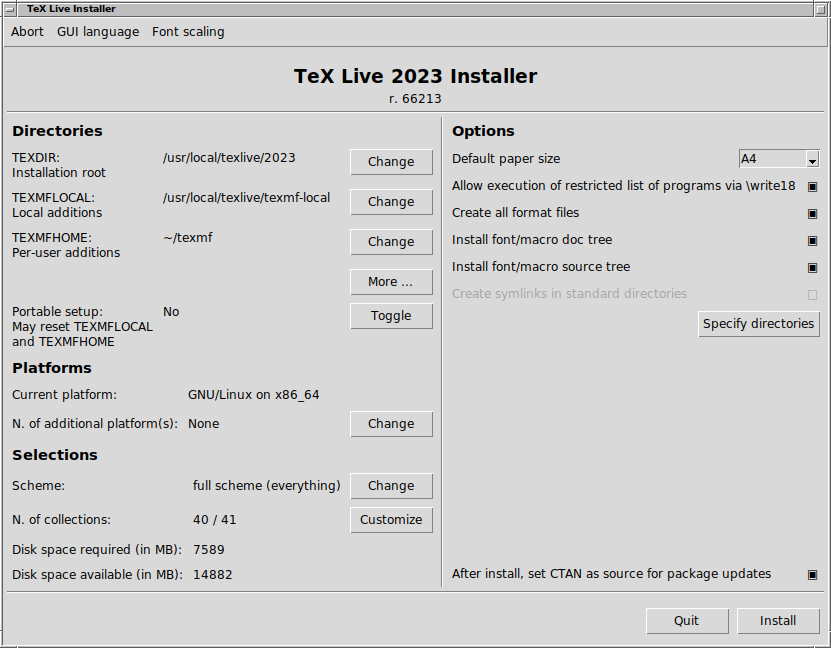
\includegraphics[width={\linewidth}]{advanced-lnx}
\caption{Fortgeschrittener GUI-Installation-Modus (\GNU/Linux)}\label{fig:advanced-lnx}
\end{figure}

\section{Cygwin}\label{sec:cygwin}

Bevor Sie mit der Installation von \TL\ beginnen, verwenden Sie das
Installationsprogramm von Cygwin (\filename{setup.exe}) um die Pakete
\filename{perl} und \filename{wget} gegebenenfalls nachzuinstallieren.
Wir empfehlen weiterhin die Installation folgender Cygwin-Pakete:

\begin{description}
\item[fontconfig] für \XeTeX und Lua\LaTeX benötigt
\item[ghostscript] wird von verschiedenen Teilen von \TL\ benötigt
\item[libXaw7] für \code{xdvi}
\item[ncurses] damit der 'clear'-Befehl im Installer funktioniert
\end{description}

\section{Installation im Textmodus}

Abb.~\ref{fig:text-main} zeigt den Eingangsbildschirm des Installationsprogramms im Textmodus (Standard unter Unix). Dieser ist ein reiner Textmodus, was zur Folge hat, dass es keine Unterstützung zum Wechseln durch die einzelnen Menüpunkte mit den Cursor-Tasten gibt. Alle Befehle, wie zum Beispiel die Auswahl von Menüpunkten, werden durch Eingabe der entsprechenden Befehle bzw.\ Menükürzel über die Tastatur eingegeben und durch \emph{Enter} übernommen. Hierbei wird zwischen Groß- und Kleinschreibung unterschieden!

Die Installation im Textmodus ist so spartanisch, weil dieser Modus überall funktionieren soll, selbst mit einer minimalen Basisinstallation von Perl.

\section{Die Installation mit grafischem Installer}

Unter Windows wird automatisch diese einfache Form der Installation verwendet,
der so genannte ">gui mode"< (Abb.~\ref{fig:wizard-w32}). Dieser zeichnet sich dadurch aus, dass er \TL\ komplett installiert und dabei vom Benutzer nur wenige Angaben gemacht werden müssen. 

Er kann mittels 

\begin{alltt}
> \Ucom{install-tl -gui}
\end{alltt}

gestartet werden.  Der Advanced-Button eröffnet Ihnen weitere Optionen (analog zum Text-Installationsmodus). %, siehe  Abbildung~\ref{fig:basic-w32}.

\subsubsection{Die Legacy-Installationsprogramme}

Die Modie\texttt{perltk}/\texttt{expert} und \texttt{wizard} sind noch auf den Systemen verfügbar, sie rufen das reguläre grafische Installationsprogramm auf.

\section{Benutzung des Installationsprogramms}\label{sec:runinstall}

Das Installationsprogramm sollte (wenn Sie die vorherigen Abschnitte zum Aufbau von \TL und der verwendeten Verzeichnisstruktur gelesen haben) weitgehend selbsterklärend sein. Trotzdem wollen wir auf einige Punkte näher eingehen.

\section{Auswahl der Binaries (nur für Unix)}\label{sec:binary}


\begin{figure}[tb]
\begin{boxedverbatim}
Available platforms:
===============================================================================
   a [ ] Cygwin on x86_64 (x86_64-cygwin)
   b [ ] MacOSX current (10.14-) on ARM/x86_64 (universal-darwin)
   c [ ] MacOSX legacy (10.6-) on x86_64 (x86_64-darwinlegacy)
   d [ ] FreeBSD on x86_64 (amd64-freebsd)
   e [ ] FreeBSD on Intel x86 (i386-freebsd)
   f [ ] GNU/Linux on ARM64 (aarch64-linux)
   g [ ] GNU/Linux on RPi(32-bit) and ARMv7 (armhf-linux)
   h [ ] GNU/Linux on Intel x86 (i386-linux)
   i [X] GNU/Linux on x86_64 (x86_64-linux)
   j [ ] GNU/Linux on x86_64 with musl (x86_64-linuxmusl)
   k [ ] NetBSD on x86_64 (amd64-netbsd)
   l [ ] NetBSD on Intel x86 (i386-netbsd)
   m [ ] Solaris on Intel x86 (i386-solaris)
   o [ ] Solaris on x86_64 (x86_64-solaris)
   p [ ] Windows (64-bit) (windows)
\end{boxedverbatim}
\caption{Auswahlmenü für Binaries}\label{fig:bin-text}
\end{figure}

\noindent Abb.~\ref{fig:bin-text} zeigt das Auswahlmenü für die Binaries der einzelnen Betriebssysteme im Textmodus. Im Allgemeinen sollte hier schon das richtige System ausgewählt sein. Sie können aber problemlos Binaries
für verschiedene Systeme parallel auswählen. Dies bietet sich an, wenn Ihre Installation auf verschiedenen Rechnern in einem heterogenen Netzwerk sichtbar ist und von dort aus benutzt werden soll.

\section{Auswahl der zu installierenden Komponenten}\label{sec:components}

\begin{figure}[tbh]
\begin{boxedverbatim}
Select scheme:
===============================================================================
 a [X] full scheme (everything)
 b [ ] medium scheme (small + more packages and languages)
 c [ ] small scheme (basic + xetex, metapost, a few languages)
 d [ ] basic scheme (plain and latex)
 e [ ] minimal scheme (plain only)
 f [ ] infrastructure-only scheme (no TeX at all)
 g [ ] book publishing scheme (core LaTeX and add-ons)
 h [ ] ConTeXt scheme
 i [ ] GUST TeX Live scheme
 j [ ] teTeX scheme (more than medium, but nowhere near full)
 k [ ] custom selection of collections
\end{boxedverbatim}
\caption{Menü zur Auswahl des Schemas}\label{fig:scheme-text}
\end{figure}


\noindent Abb.~\ref{fig:scheme-text} zeigt das Auswahlmenü für ein grundsätzliches Installationsschema der
\TL. Durch die Auswahl eines Schemas werden automatisch die Komponenten zur Installation ausgewählt, die
für das gewünschte Schema notwendig bzw.\ sinnvoll sind. Mit einer vollständigen Installation von \TL
(\emph{full scheme}) sind Sie auf der sicheren Seite, da hier einfach alles installiert wird, auch die Unterstützung für Dinge, die Sie vermutlich niemals brauchen werden. Sie können aber auch eines der abgespeckten Schemas wie \emph{basic} (für ein sehr schlankes System), \emph{small}
oder \emph{minimal} (dies empfiehlt sich aber nur für Testsysteme und weniger zum ernsthaften Arbeiten)
auswählen. Weiter stehen einige Schemata für spezielle Anwendungszwecke oder Sprachen zur Verfügung.

\begin{figure}[tb]
\begin{center}
\includegraphics[width=.9\linewidth]{stdcoll}
\caption{Menü zur Aus- oder Abwahl von Collections.}\label{fig:collections-gui}
\end{center}
\end{figure}

Wenn Sie das Schema ausgewählt haben, können Sie dieses in den Menüpunkten \emph{standard collections} und
\emph{language collections} (s.\,Abb.~\ref{fig:collections-gui}, diesmal zur Abwechslung im GUI-Modus)
individuell nach Ihren Wünschen anpassen.

Während das Schema nur den grundlegenden Funktionsumfang vorgibt, ist die Auswahl von Komponenten auf der
Ebene der \emph{Collections} viel feiner. Eine Collection besteht dabei aus mehreren Paketen zu einem Thema,
wobei jedes der Pakete aus bestimmten Makrodateien, Fontdateien usw. bestehen kann.

Noch mehr Kontrolle über die Komponenten Ihres Systems haben Sie nach der Installation mit dem \TeX\ Live Manager (\prog{tlmgr}), das in Kapitel~\ref{sec:tlmgr} beschrieben wird. Hier können Sie gezielt einzelne Pakete installieren oder entfernen.

\section{Verzeichnisse}\label{sec:directories}


Die Verzeichnisstruktur von \TL wurde bereits im Kapitel~\ref{sec:texmftrees} auf S.~\pageref{sec:texmftrees}
beschrieben. Als Wurzelverzeichnis für \TL (\dirname{TEXDIR}) wird unter Windows
\verb|%SystemDrive%\texlive\2023| und unter Unix (\dirname{/usr/local/texlive/2023}) angenommen. 

Prinzipiell können Sie diesen Pfad problemlos ändern, z.\,B. wenn Sie \TL als Standardnutzer und nict als Admin installieren wollen bzw. keine Schreibrechte in dem oben angegebenen Verzeichnis besitzen.

Auf Wunsch können Sie \TL also auch in Ihrem Home-Verzeichnis installieren, wenn Sie sowieso der einzige Nutzer von \TL auf Ihrem Rechner sind. Für Ihr Home-Verzeichnis können Sie den Pfad ">|~|"< verwenden und so beispielsweise \TL nach  |~/texlive/2023| installieren.

Wir empfehlen Ihnen, die Jahreszahl im Verzeichnisnamen beizubehalten. So können Sie von Jahr zu Jahr einfach die neue Version testen, ohne die alte zu entsorgen. Bei Bedarf können Sie einen symbolischen
Link (z.B. \dirname{/usr/local/texlive-cur}) verwenden, der jeweils auf das Verzeichnis der aktuellen Version von \TL verweist.

Wenn Sie die Einstellung \dirname{TEXDIR} im Installationsprogramm ändern, werden die Werte für
\dirname{TEXMFLOCAL}, \dirname{TEXMFSYSVAR} und \dirname{TEXMFSYSCONFIG} automatisch angepasst. In Abbildung \ref{fig:advanced-lnx} finden Sie eine Übersicht der entsprechenden Optionen.

Das als \dirname{TEXMFHOME} bezeichnete Verzeichnis ist der Ort, in dem persönliche Makrodateien,
Schriften o.\,ä. abgelegt werden können. Vorgabewert ist \textasciitilde/texmf. Im Gegensatz zu \dirname{TEXDIR} wird \textasciitilde\ hier nicht direkt zum Pfad des Home-Verzeichnisses aufgelöst, sondern unverändert in die Konfigurationsdateien von \TL übernommen und erst zur Laufzeit aufgelöst. Somit kann jeder Nutzer des Systems seinen komplett eigenen Pfad haben, der von \TL verwendet wird, und so nach Wunsch auch eigene Konfigurationsänderungen durchführen. Zur Laufzeit wird \textasciitilde\ unter Unix durch \dirname{\$HOME} und unter Windows durch \verb|%USERPROFILE%| ersetzt.

Die Variable \dirname{TEXMFVAR} verweist auf das Verzeichnis mit benutzerspezifisch
erzeugten Konfigurationsdateien, z.\,B. den Konfigurations-Cache von \ConTeXt\ Mk\acro{IV}.

\clearpage

\section{Optionen}\label{sec:options}

Der folgende Rahmen zeigt das Menü, in dem weitere Einstellungen für die Installation von \TL möglich sind.

\begin{boxedverbatim}
 <P> use letter size instead of A4 by default: [ ]
 <E> execution of restricted list of programs: [X]
 <F> create all format files:                  [X]
 <D> install font/macro doc tree:              [X]
 <S> install font/macro source tree:           [X]
 <L> create symlinks in standard directories:  [ ]
            binaries to:
            manpages to:
                info to:
 <Y> after install, set CTAN as source for package updates: [X]
\end{boxedverbatim}
%\label{fig:options-text}


 Zur Erläuterung:
\begin{description}
\item[use letter size instead of A4 by default:] Verwendung von Letter anstatt DIN\,A4 als
Standard\-papier\-größe. Natürlich können Sie später unabhängig davon für einzelne Dokumente eine
beliebige Papiergröße wählen.

\item[execution of restricted list of programs:] Seit \TL\ 2011 können bei einem
\TeX-Lauf standardmäßig einige externe Programme aufgerufen werden. Die (kurze) 
Liste der erlaubten Programme wird in der Datei \filename{texmf.cnf} definiert.
Für weitere Informationen siehe Kapitel~\ref{sec:2011news} über Neuerungen in 
\TL\ 2011.

\item[create all format files:] Auch wenn das Erzeugen von Formatdateien für Makropakete, die Sie gar nicht benötigen, Zeit und Platz kostet, empfehlen wir trotzdem, diese Option ausgewählt zu belassen.  Falls Sie diese Option abwählen, werden Formatdateien jeweils bei Bedarf erzeugt, und dann im persönlichen \dirname{TEXMFVAR}-Baum des aktuellen Benutzers abgelegt. Dort liegende Formate werden allerdings nicht automatisch neu generiert. Wenn z.\,B. Programme oder Silbentrennmuster aktualisiert werden, dann kann es zu Inkompatibilitäten kommen. 

\item[install font/macro \ldots\ tree:] Mit dieser Option können Sie  verhindern, dass die Dokumentation und die Quelldateien der Pakete  installiert werden. Wir raten aber, die Vorgabe zu übernehmen, d.\,h. die Dokumentation und Quelldateien zu installieren.

\item[create symlinks in standard directories] (nur unter Unix):
  Mit dieser Option können Sie symbolische Links für Programme und Dokumentation in den Standard\-verzeichnissen   Ihres Systems anlegen, so dass Sie Ihre Umgebungsvariablen \envname{PATH}, \envname{MANPATH} und \envname{INFOPATH} nicht anpassen müssen. Sie benötigen für diese Option Schreibrechte in den entsprechenden Verzeichnissen. Hinweis: Diese Option ist nicht dazu gedacht, ein vorhandenes \TeX-System, das zum Beispiel als Teil Ihrer Linux-Distribution installiert wurde, zu überschreiben! Sie dient vielmehr dazu, dass Links in Verzeichnissen angelegt werden, wo die Nutzer sie erwarten -- beispielsweise in \dirname{/usr/local/bin} --, aber sich dort noch keine \TeX-Programme befinden.

\item[after installation \dots{} CTAN:] Diese Option ist bei der Installation von DVD standardmäßig gesetzt. Sie sorgt dafür, dass nach der Installation Paket-Ak\-tuali\-sie\-rungen aus dem Internet geladen werden. Es gibt nur einen sinnvollen Grund, diese Option nicht zu aktivieren: wenn nur eine Untermenge von \TL\ installiert wurde und Pakete nach der Installation manuell hinzugefügt werden sollen.
\end{description}

Windows-spezifische Optionen sind wie folgt: 

\begin{description}
\item[Pass die PATH Variable in der Registry an] Sorgt dafür, dass alle Programme die \TeX-Programme im Pfad finden können.

\item[Füge Menüeinträge hinzu] Fügt bei gesetzter Option Menü-Einträge in das Startmenü ein.
Beschrieben in \ref{sec:sharedinstall}.

\item[Ändere Datei-Verknüpfungen] Optionen sind hier `Only new' (erstelle Verknüpfungen, aber überschreibe nicht existierende Verknüpfungen), `Alle' und `Keine'.

\item[Installiere \TeX{}works] Installiert bei gesetzter Option \TeX works
\end{description}

\noindent Wenn Sie alle gewünschten Einstellungen für die Installation vorgenommen haben, können Sie im Hauptmenü nun ">I"< eintippen, um diese zu starten. Lesen Sie dann anschließend Kapitel~\ref{sec:postinstall} für
eventuell notwendige Arbeiten zum Abschluss der Installation.

\section{Kommandozeilenoptionen für die Installation}\label{sec:cmdline}


Nach Eingabe von
\begin{alltt}
> \Ucom{install-tl -help}
\end{alltt}
erhalten Sie eine Liste der vorhanden Kommando\-zeilen\-optionen.  Sie können diese entweder mit |-| oder |--|
verwenden. Die wichtigsten sind:

\begin{description}
\item[-gui] Nutze wenn möglich die grafische Oberfläche. Dies benötigt Tcl/TK 8.5  oder höher. Tcl/TK 8.5 ist nur Teil von \macOS bis Monterey, danach müssen Sie es selbst installieren. Die Legacy-Optionen \texttt{-gui=perltk} und \texttt{-gui=wizard} sind noch verfügbar, aber rufen die gleiche grafische Benutzeroberfläche auf.  Wenn Tcl/Tk nicht verfügbar ist, wird die Installation im Textmodus durchgeführt.

\item[-no-gui] Installation im Textmodus. Da dies unter Unix Standard ist, wirkt sich diese Option nur
  unter Windows aus. Da die Installation zum Benutzen von \TL direkt von \DVD im grafischen Modus nicht
  verfügbar ist, brauchen Sie in diesem Fall unbedingt den Textmodus.

\item[-lang {\textsl{LL}}] Sprache des Installationsprogramms als Sprach-Code in zwei Buchstaben (\textsl{LL}).
  Derzeit werden unterstützt. Das Installationsprogramm versucht, die gewünschte Sprache anhand des
  Systems herauszufinden. Falls dies scheitert oder die betreffende Sprache nicht verfügbar ist, wird als
  Fallback-Sprache Englisch genutzt.

\item[-portable] Die Option \code{-portable} (\code{V} im Text-Installer oder die gleiche Option im grafischen Installer);  dient der Installation auf einem USB-Stick oder einer DVD-R. Siehe Kapitel \ref{sec:portable-tl} für Informationen über die portable Installation von \TL.

\item[-profile {\textsl{profile}}] Das Installationsprogramm schreibt die ausgewählten Optionen in eine Datei
  \filename{texlive.profile}. Mit dieser Option können
  Sie eine bereits vorhandene Datei bei der Installation weiter verwenden, z.\,B. wenn Sie äquivalente
  Installationen auf mehreren Rechnern realisieren wollen, ohne alle Auswahlschritte der Installation immer
  wieder neu durchführen zu müssen.

\item [-repository {\textsl{url/path}}] zur Auswahl einer Installationsquelle,
  für weitere Erläuterung siehe den nächsten Kapitel.


\item[-in-place] Sollten Sie schon ein rsync, svn, oder eine andere Kopie von 
  \TL{} haben (siehe \url{https://tug.org/texlive/acquire-mirror.html}), dann wird diese Option genau das nutzen, was Sie schon haben und nur die notwendigen post-install Operationen durchführen. Eine Warnung: Die Datei \newline \filename{tlpkg/texlive.tlpdb} kann dadurch überschrieben werden; machen Sie vorher gegebenenfalls eine Sicherheitskopie. Die Entfernung von Paketen muss auch manuell vorgenommen werden. 
	
Diese Option kann nicht über die Installer-Schnittstelle gesetzt werden.
\end{description}

\section{Die Option repository}\label{sec:location}


Als Standardquelle für die Installation wird ein \CTAN-Knoten verwendet, der automatisch von \url{https://mirror.ctan.org} ermittelt wird.

Falls Sie eine andere Installationsquelle verwenden wollen, geben Sie eine neue Quelle an, die entweder mit \texttt{ftp:}, \texttt{http:}, \texttt{https:} oder \texttt{file:/} beginnt oder ein Verzeichnispfad auf Ihrem System ist.
Falls Sie \texttt{http:}, \texttt{https:} oder \texttt{ftp:} verwenden, werden ">\texttt{/}"<-Zeichen oder ein ">\texttt{/tlpkg}"<- am Ende ignoriert.

Sie können also z.\,B. einen bestimmten \CTAN-Knoten auswählen, so etwa
\url{https://ctan.example.org/tex-archive/systems/texlive/tlnet/},
wobei Sie natürlich statt |ctan.example.org| einen echten Servernamen
verwenden und wahrscheinlich auch den Rest der URL anpassen müssen.
Eine Auflistung von \CTAN-Servern finden Sie unter \url{https://ctan.org/mirrors}.

Falls Sie ein lokales Repository verwenden (also entweder direkt einen
Verzeichnispfad oder eine \texttt{file:/}-URL angeben), dann werden
bevorzugt Archivdateien in einem Unterverzeichnis \dirname{archive} des
Repository verwendet, selbst wenn ausgepackte Dateien vorhanden sind.

\section{Aufgaben im Anschluss an die Installation}\label{sec:postinstall}

Je nach System kann es notwendig sein, dass im Anschluss an die Installation noch einige Kleinigkeiten erledigt werden müssen.

\subsection{Windows}

Benutzer von Windows sind hier in der glücklichen Position, dass das Installationsprogramm alles komplett erledigt haben sollte.

\subsection{Unix, falls symbolische Links angelegt wurden}

Wenn Sie bei der Installation angegeben haben, dass und wo symbolische Links angelegt werden sollten (siehe Kapitel~\ref{sec:options}), dann sollten hier auch keine Nacharbeiten mehr notwendig sein.

\subsection{Umgebungsvariablen für Unix}
\label{sec:env}

Das Verzeichnis mit den ausführbaren Programmen von \TL muss sich im Suchpfad des Systems befinden.
Jedes unterstützte System besitzt ein eigenes Verzeichnis unterhalb von \dirname{TEXDIR/bin}, deren
Namen Sie in Abb.~\ref{fig:bin-text} finden.

Weiterhin können Sie die Verzeichnisse mit den Manual-Pages und Info-Dateien zu den entsprechenden
Suchpfaden für Dokumentation hinzufügen.

Für Systeme mit einer Bourne-kompatiblen Shell wie \prog{bash} ist hier am Beispiel von GNU/Linux
aufgeführt, wie die Befehle zum Setzen der Umgebungsvariablen (z.\,B. in \filename{\$HOME/.profile})
aussehen könnten:

\begin{verbatim}
PATH=/usr/local/texlive/2023/bin/x86_64-linux:$PATH; export PATH
MANPATH=/usr/local/texlive/2023/texmf-dist/doc/man:$MANPATH; export MANPATH
INFOPATH=/usr/local/texlive/2023/texmf-dist/doc/info:$INFOPATH; export INFOPATH
\end{verbatim}


\noindent Für \prog{csh} oder \prog{tcsh} erfolgt die Konfiguration in der Regel in der Datei~\filename{\$HOME/.cshrc}
und könnte so aussehen:

\begin{verbatim}
setenv PATH /usr/local/texlive/2023/bin/x86_64-linux:$PATH
setenv MANPATH /usr/local/texlive/2023/texmf-dist/doc/man:$MANPATH
setenv INFOPATH /usr/local/texlive/2023/texmf-dist/doc/info:$INFOPATH
\end{verbatim}

\subsection{Systemweites Setzen von Umgebungsvariablen}
\label{sec:envglobal}


Wenn Sie als Administrator die Umgebungsvariablen global für das gesamte System setzen wollen,
gehen wir davon aus, dass Sie sich mit der grundlegenden Systemadministration auskennen.

Daher hier nur zwei Hinweise: 

\begin{enumerate}
\item Schauen Sie nach einer Datei
\filename{/etc/manpath.config}. Falls diese vorhanden ist, sollte es reichen, folgende Zeilen
hinzu zu fügen:

\begin{verbatim}
MANPATH_MAP /usr/local/texlive/2023/bin/ix86_64-linux \
            /usr/local/texlive/2023/texmf-dist/doc/man
\end{verbatim}

\item Prüfen Sie, ob es auf Ihrem System eine Datei \filename{/etc/environment} gibt, in der die
systemweiten Umgebungsvariablen definiert werden.

Zusätzlich wird ein symbolischer Link \code{man} im binary-Verzeichnis unter
Unix angelegt, der auf \dirname{texmf-dist/doc/man} verweist. Einige Versionen von \code{man}, so z.\,B. unter \macOS, finden so verlinkte Man-Pages automatisch, so dass hier keine spezielle
Konfiguration für die Man-Pages mehr erforderlich ist.

\end{enumerate}

\subsection{Internet-Updates nach der Installation von DVD}
\label{sec:dvd-install-net-updates}


Wenn Sie von DVD installiert haben, können Sie mittels des folgenden Befehls die Aktualisierung über das Internet aktivieren. Zuerst müssen Sie, wie im vorhergehenden Kapitel beschrieben, den Suchpfad angepasst haben:

\begin{alltt}
> \Ucom{tlmgr option repository https://mirror.ctan.org/systems/texlive/tlnet}
\end{alltt}

\noindent Dadurch nutzt \cmdname{tlmgr} beim nächsten Update einen \CTAN\ Mirror. Sollte es Probleme bei der automatischen Wahl eines Mirror-Servers geben, kann ein bestimmter \CTAN\ Server von der unter \url{https://ctan.org/mirrors} verfügbaren Liste ausgewählt werden. Benutzen Sie diesen Pfad dann mit dem oben genannten Befehl.

\subsection{Font-Konfiguration für xe\TeX\ und Lua\TeX2}\label{sec:font-conf-xetex}

\XeTeX\  und Lua\TeX\ können nicht nur die Schriften in den \TeX\ Bäumen nutzen, sondern auch die auf dem System vorhandenen Fonts. Die Methoden, wie sie dies tun, ähneln sich, sind aber verschieden.

Unter Windows sind die auf dem System vorhandenen Schriften automatisch nutzbar. Auf einem Unix/Linux System sind Anpassungen notwendig, damit die Schriften über den Systemname und nicht nur Dateinamen gefunden werden können.

Hierfür wird bei der Installation des \filename{xetex} Pakets die Datei \newline  \filename{TEXMFSYSVAR/fonts/conf/texlive-fontconfig.conf}
erzeugt.

Um die mitgelieferten \TL-Schriften systemweit verwenden zu können,
gehen Sie bitte folgendermaßen vor:

\begin{enumerate}
\item Kopieren Sie als root-User \filename{texlive-fontconfig.conf} nach \newline
\dirname{/etc/fonts/conf.d/09-texlive.conf}.
\item Führen Sie \Ucom{fc-cache -fsv} aus. 
\end{enumerate}

\noindent Falls Ihnen als normaler Nutzer die entsprechenden Rechte für die
obigen Schritte fehlen, können Sie die \TL-Schriften für sich selbst
als \XeTeX-Nutzer verwendbar machen:

\begin{enumerate}
\item Kopieren Sie \filename{texlive-fontconfig.conf} in das Unterverzeichnis
      \filename{\textasciitilde/.fonts.conf}, wobei \textasciitilde\ Ihr Home-Verzeichnis ist.
\item Führen Sie \Ucom{fc-cache -fv} aus.
\end{enumerate}

Führen Sie \code{fc-list} aus, um eine Liste der Systemschriften mit hilfreichen Informationen zu erhalten.

\subsection{Con\TeX t Mark IV}
\label{sec:context-mkiv}

Sowohl das \enquote{alte} \ConTeXt{} (Mark \acro{II} und Mark \acro{IV}) als auch das \enquote{neue} \ConTeXt{} (LMTX) sollten problemlos nach der \TL{} Installation funktionieren und brauchen keine besondere Aufmerksamkeit, sofern \verb+tlmgr+ für den Update-Prozess genutzt wird.

Da \ConTeXt{}  jedoch nicht die kpathsea-Bibliothek nutzt, ist
ein wenig manuelle Nacharbeit notwendig, wenn neue Dateien manuell installiert werden (also ohne die Nutzung von \verb+tlmgr+).

Nach einer jeden solchen Installation muss jeder Nutzer das das folgende Kommando ausführen, um den \ConTeXt{} Cache zu aktualisieren:

für LMTX

\begin{verbatim}
context --generate
\end{verbatim}

für Mark \acro{IV}

\begin{verbatim}
context --luatex --generate
\end{verbatim}



Die erzeugten Dateien werden in \code{TEXMFCACHE} gespeichert, dessen Standardwert \verb+TEXMSYSVAR;TEXMFVAR+ ist. 

\ConTeXt\ liest aus allen Pfaden, die in \verb+TEXMFCACHE+ aufgeführt sind und schreibt in die erste Pfadangabe, bei der Schreibrechte existieren. Im Fall identischer Cache-Daten hat der letzte gefundene Pfad Vorrang vor allen anderen Pfaden.

Für weitere Informationen siehe \url{https://wiki.contextgarden.net/LMTX}\\
und \url{https://wiki.contextgarden.net/Running_Mark_IV}.

\subsection{Integration lokaler bzw. nutzer-spezifischer Makros}
\label{sec:local-personal-macros}

Wie bereits in Kapitel~\ref{sec:texmftrees} erwähnt, ist der Verzeichnisbaum \dirname{TEXMFLOCAL} (im Normalfall \dirname{/usr/local/texlive/texmf-local} oder \verb|%SystemDrive%\texlive\|\newline \verb|texmf-local|) für lokale Ergänzungen wie Makros und Schriften gedacht, die anschließend allen Benutzern des Systems zur Verfügung stehen. Weiterhin können Benutzer den Verzeichnisbaum \dirname{TEXMFHOME} (im Normalfall \dirname{\$HOME/texmf} oder \verb|%USERPROFILE%\texmf|) für persönliche Ergänzungen verwenden, ohne dass andere Benutzer davon beeinflusst werden.

Diese Verzeichnisse sollen über verschiedene Versionen von \TL hinweg identisch sein, so dass ein Update von \TL auf eine neue Version einfach möglich ist, ohne dass Sie Ihre lokalen Ergänzungen verlieren. Wir empfehlen Ihnen daher, von der vorgegebenen Verzeichnisstruktur nicht abzuweichen.

Für beide oben genannte Verzeichnisbäume erwartet \TL eine Verzeichnisstruktur innerhalb des Baums, die dem \emph{\TeX{} Directory Standard} entspricht, wie er in \url{https://tug.org/tds} bzw. \filename{texmf-dist/web2c/texmf.cnf} definiert ist.
So gehören Dokumentklassen für \LaTeX{} zum Beispiel in ein Verzeichnis
unterhalb von \dirname{TEXMFLOCAL/tex/latex} oder \dirname{TEXMFHOME/tex/latex}.

Der Verzeichnisbaum \dirname{TEXMFLOCAL} wird zur Laufzeit nicht direkt nach Dateien durchsucht. Stattdessen wird eine Liste von Dateinamen verwendet, sich sich in einer Datei mit dem Namen~\filename{ls-R} befindet. Denken Sie also daran, nach Änderungen in diesem Baum diese Dateiliste zu aktualisieren. Dies tun Sie
entweder mit dem Befehl \cmdname{mktexlsr} oder über die Schaltfläche \emph{Reinit file database} im Kon\-fi\-gu\-rations\-reiter des \TeX\ Live Managers (GUI-Modus).

\subsection{Integration von Schriften}

Die Installation von Schriften für pdf\TeX, die nicht Bestandteil von \TL sind, ist eine recht komplexe Angelegenheit. Lassen Sie es am besten sein, wenn Sie sich nicht sehr gut mit dem System auskennen! % Schauen Sie vielleicht vorher in Kapitel~\ref{sec:tl-fonts} nach, welche Schriften bereits bei \TL mitgeliefert werden.

Eine Alternative besteht in der Nutzung von \XeTeX\ oder Lua\TeX\ (s.\,Kapitel~\ref{sec:tex-extensions}), bei dem direkt alle vom Betriebssystem installierten Schriften verwendet werden können, ohne dass die Installation einer \TeX-Unterstützung notwendig ist.

Falls Sie wirklich weitere Schriften benötigen, finden Sie unter \url{https://tug.org/fonts/fontinstall.html} eine Beschreibung zur
Installation weiterer Schriften.

\section{Testen der Installation}
\label{sec:test-install}


Nach der Installation von \TL wollen Sie es natürlich benutzen, um möglichst schöne Dokumente zu setzen.

Dieser Kapitel beschreibt, wie Sie prüfen können, ob Ihr \TL-System funktioniert.
Die folgenden Beispiele sind für Unix, sollten unter Windows und \macOS\ aber sehr ähnlich sein. Der Unterschied kann sein, dass Sie dort eventuell eine grafische Benutzeroberfläche verwenden. 
Unter Windows installiert \TL \TeX works, unter Mac OS X \TeX Shop (siehe \url{https://pages.uoregon.edu/koch/texshop}.  Auf anderen Linux/Unix-Systemen obliegt es dem Nutzer, einen Editor auszuwählen. 
Im Grunde funktioniert jeder normaler Editor, ein Unicode-fähiger Editor wird aber sehr empfohlen.

\begin{enumerate}

\item Prüfen Sie, ob Sie das Programm \cmdname{tex} ausführen können:

\begin{alltt}
> \Ucom{tex -{}-version}
TeX 3.14159265 (TeX Live ....)
Copyright .... D.E. Knuth.
...
\end{alltt}

Erhalten Sie als Resultat statt der Versionsnummer die Meldung, dass der Befehl nicht gefunden wurde,
so haben Sie wahrscheinlich vergessen, das Verzeichnis mit den ausführbaren Programmen
in Ihren \envname{PATH} aufzunehmen, siehe Kapitel~\ref{sec:env} auf Seite~\pageref{sec:env}.

\item Eine einfache \LaTeX{}-Datei übersetzen:
\begin{alltt}
> \Ucom{pdflatex sample2e.tex}
This is pdfTeX, Version 3.14...
...
Output written on sample2e.pdf (3 pages, 7484 bytes).
Transcript written on sample2e.log.
\end{alltt}

Falls dies schief geht, sind wahrscheinlich noch alte Umgebungsvariablen einer vorigen \TeX-Installation
übrig geblieben. Wir empfehlen, die Umgebungsvariablen, die sich auf \TeX{} beziehen, zu entfernen.
Für eine weitere Analyse können Sie \TeX{} anzeigen lassen, wo es bestimmte Dateien sucht,
siehe \enquote{Fehlersuche} auf Seite~\pageref{sec:debugging}.

\item Ergebnis auf dem Bildschirm anschauen:
\begin{alltt}
> \Ucom{xpdf sample2e.pdf}    
\end{alltt}

Nun sollte sich ein Vorschaufenster mit dem soeben gesetzten Beispieldokument öffnen, das die Grundlagen von \LaTeX{} erläutert (und das Anfänger tatsächlich auch einmal lesen sollten). Es gibt verschiedene empfehlenswerte PDF Viewer: unter Windows empfehlen wir Sumatra PDF (\url{https://www.sumatrapdfreader.org/free-pdf-reader.html}), unter Linux/Unix \cmdname{evince} und \cmdname{okular}.

Sie können auch anstelle des PDF eine DVI Datei erzeugen 

\begin{alltt}
> \Ucom{latex sample2e.tex}    
\end{alltt}

und diese mit dem eingebauten DVI-Viewer anschauen.

\begin{alltt}
> \Ucom{xdvi sample2e.dvi}    
\end{alltt}

Unter Unix muss ein X-Server laufen, damit \cmdname{xdvi} funktioniert; falls dies nicht der Fall ist oder die Umgebungsvariable \envname{DISPLAY} falsch gesetzt ist, erhalten Sie die Fehlermeldung \samp{Can't open display}.

\item Eine \PS{}-Datei aus der \dvi erzeugen:
\begin{alltt}
> \Ucom{dvips sample2e.dvi -o sample2e.ps}
\end{alltt}

Weder \cmdname{gv} noch \cmdname{xpdf} sind in \TL{} enthalten, daher müssen diese separat installiert
werden, siehe \url{https://www.gnu.org/software/gv} bzw. \url{https://www.foolabs.com/xpdf}.

Sie können natürlich auch andere PDF-Viewer verwenden, beispielsweise Adobe Reader. Dieser hat allerdings unter Windows das Problem, dass geöffnete PDF-Dateien nicht überschrieben werden können. Dies führt zu Fehlern von pdf\TeX, wenn Sie ein Dokument übersetzen wollen und vergessen haben, es vorher im Adobe Reader zu schließen. Unter Windows sollten Sie daher auch einmal Sumatra PDF (\url{https://blog.kowalczyk.info/software/sumatrapdf}) ausprobieren, der dieses Problem nicht hat und deutlich weniger Ressourcen braucht als Adobe Reader.

\item Weitere nützliche Test-Dateien außer
\filename{sample2e.tex}:

\begin{description}
\item [small2e.tex] Einfachere Version von \filename{sample2e}, um den Fehler einzugrenzen, wenn Sie
beim Übersetzen von \filename{sample2e} Probleme haben.
\item [testpage.tex] Hiermit können Sie prüfen, ob Ihr Drucker Ihren Ausdruck horizontal oder vertikal verschiebt.
\item [nfssfont.tex] Zum Testen von Fonts und Erzeugen von Schrifttabellen.
\item [testfont.tex] Erzeugen von Schrifttabellen, aber mit plain \TeX.
\item [story.tex] Das einfachste Testdokument von allen (in plain \TeX{}).
Geben Sie am Ende \samp{\bs bye} ein, wenn nach dem Aufruf von \samp{tex
story.tex} der \code{*} erscheint.
\end{description}

\item Falls Sie das \filename{xetex}-Paket installiert haben, können Sie
das Verwenden von Systemschriften folgendermaßen testen:
\begin{alltt}
+> \Ucom{xetex opentype-info.tex}
This is XeTeX, Version 3.1415926\dots
...
Output written on opentype-info.pdf (1 page).
Transcript written on opentype-info.log.
\end{alltt}

(Oder das gleiche für \filename{luatex}.)

Falls Sie die Fehlermeldung \enquote{Invalid fontname 'Latin Modern
Roman/ICU'\dots} erhalten, muss Ihr System so konfiguriert werden, dass
es die von \TL\ mitgelieferten Schriften findet. % (siehe Kapitel~\ref{sec:font-conf-sys}).
\end{enumerate}

\section{\TL Deinstallieren}
\label{sec:uninstall}

Um \TL\ nach einer erfolgreichen Installation zu deinstallieren, führen Sie

\begin{alltt}
> \Ucom{tlmgr uninstall --all}
\end{alltt}

aus. Sie müssen dies bestätigen, sonst erfolgt keine Deinstallation. Hinweis:
Ohne die \code{-{}-all} Option wird der Schalter \code{uninstall} genutzt, um einzelne Pakete zu deinstallieren.

Der Befehl löscht keine benutzerspezifischen Verzeichnisse, siehe section~{sec:texmftrees}:

\begin{description}
\item [TEXMFCONFIG] Dieses Verzeichnis enthält Konfigurationsanpassungen auf Nutzer-Ebene. Wenn sie erhalten bleiben sollen, sichern Sie sie vorher.

\item [TEXMFVAR] Dieses Verzeichnis enthält zum Beispiel lokale Formatdateien. Wenn Sie es nicht noch zu anderen Zwecken genutzt haben, dann ist das Löschen kein Problem.

\item[TEXMFHOME] Enthält Dateien, die Sie persönlich der TeX Installation hinzugefügt haben. Sie sollten dieses Verzeichnis nur löschen, wenn Sie kein TeX mehr nutzen möchten.

\end{description}

\noindent Die Verzeichnisse für diese Variablen können Sie mittels \code{kpsewhich -var-value=\code{var}} abfragen.

Die \prog{tlmgr} Deinstallation nimmt keine Anpassungen der Pfad-Umgebungsvariablen und Systemzugriffen für Schriftaren vor (siehe 
Abschnitt~\ref{sec:postinstall}). Diese Schritte müssen Sie manuell vornehmen, sofern gewünscht.

Unter Windows kann die Deinstallation von TeX Live über die grafische Oberfläche vorgenommen werden, siehe Abschnitt~\ref{sec:winfeatures}.

\section{Hinweise auf weitere Software}

In vielen Fällen ist die Installation weiterer Software sinnvoll:

\begin{description}
\item[Ghostscript] \url{https://www.cs.wisc.edu/~ghost/}, ein freier PostScript und PDF Interpreter
\item[Perl] \url{https://www.perl.org/} mit Zusatzpaketen von
      \acro{CPAN}, \url{https://www.cpan.org/},
\item[ImageMagick] \url{https://www.imagemagick.com}, für die Bearbeitung
      und Umwandlung von Bildern in andere Formate,
\item[NetPBM] \url{https://netpbm.sourceforge.net/}, ebenfalls für Bilder.

\item[\TeX-Oberflächen] Es gibt eine breite Auswahl von Oberflächen bzw.
     Editoren, die \TeX\ unterstützen, je nach persönlichem Geschmack des
     Benutzers. Hier ist eine Auswahl, wobei einige davon nur für Windows verfügbar sind:
  \begin{itemize}
  \item \cmdname{GNU Emacs}, ein sehr guter Editor siehe
        \url{https://www.gnu.org/software/emacs/emacs.html}.
  \item \cmdname{Emacs} mit Auc\TeX\ für Windows findet man auf der Homepage  \url{https://www.gnu.org/software/auctex}.
  \item \cmdname{LEd} findet sich unter \url{https://www.latexeditor.org/}.
  \item \cmdname{SciTE} findet sich unter
        \url{https://www.scintilla.org/SciTE.html}.
  \item \cmdname{Texmaker} ist Freie Software, verfügbar über
        \url{https://www.xm1math.net/texmaker}.
  \item \cmdname{TeX Studio} \url{https://texstudio.sourceforge.net}
        ist eine Version von \cmdname{Texmaker} mit zusätzlichen Features
  \item \cmdname{TeXnicCenter} ist Freie Software, verfügbar über
        \url{https://www.texniccenter.org}
  \item \cmdname{TeXworks} ist Freie Software, verfügbar über
        \url{https://tug.org/texworks}. Wird unter Windows und
        \macOS\ als Teil von \TL\  mitinstalliert.
  \item \cmdname{Vim} ist freie Software, verfügbar über
        \url{https://www.vim.org}.
  \item \cmdname{WinShell} findet sich unter \url{https://www.winshell.de}.
  \item \cmdname{WinEdt} ist Shareware, verfügbar über
        \url{https://tug.org/winedt} oder \url{https://www.winedt.com}.
        Bitte beachten Sie, dass es für Mitglieder von \dante\ ein
        Lizenzabkommen mit WinEdt zu sehr günstigen Preisen gibt. 
  \end{itemize}
\end{description}
Für weitere Programme siehe \url{https://tug.org/interest.html}.

\chapter{Installation für mehrere Maschinen oder Nutzer (Netz-Installation)}
\label{sec:sharedinstall}

Bei \TL ist nicht nur vorgesehen, dass es von mehreren Benutzern auf einem System verwendet werden kann, sondern auch in einem Netzwerk. In der normalen Konfiguration von \TL werden nur relative und keine absoluten Pfade verwendet. Dies erkennt man an Einstellungen in der Datei {\small \filename{\$TEXMFDIST/web2c/texmf.cnf}}, die Zeilen wie die folgenden enthält, in denen Verzeichnisse relativ zu den Verzeichnissen lokalisiert werden, in denen sich die Programme befinden:

\begin{verbatim}
TEXMFROOT = $SELFAUTOPARENT/texmf
...
TEXMFDIST = $TEXMFROOT/texmf-dist
...
TEXMFLOCAL = $SELFAUTOPARENT/../texmf-local
\end{verbatim}

Daher ist es im Normalfall ausreichend, das Programm-Verzeichnis in den Suchpfad des Systems aufzunehmen, alles weitere bestimmt \TL dann automatisch.

Daher ist es kein Problem, wenn das Grundverzeichnis von \TL als Netz\-lauf\-werk eingebunden ist. Tatsächlich können Sie \TL\ sogar zunächst lokal installieren und dann auf ein Netzlaufwerk verschieben.

Für Benutzer von Windows enthält \TL{} einen Launcher \filename{tlaunch}. Sein Hauptfenster enthält Menü-Einträge und Buttons für verschiedene \TeX-Programme und Dokumentationen, anpassbar via ini-Datei.
Mehr Informationen dazu unter (\code{texdoc tlaunch} oder \url{https://ctan.org/pkg/tlaunch}).


\chapter{Portables \TL  auf DVD oder USB-Stick}\label{sec:portable-tl}

Wenn Sie \TL\ im portablen Modus verwenden wollen (z.\,B. auf einem Rechner, auf dem Sie "`Gast"' sind), können Sie \TL\ mit der Option \optname{-portable} (bzw. der Option \code{V} im Text-Installer oder der entsprechenden Option im grafischen Installer) auf einem USB-Stick installieren (siehe Kapitel \ref{sec:cmdline}). 

Vom technischen Standpunkt aus betrachtet wird die portable Installation so erzeugt, dass die Standardwerte für \envname{TEXMFHOME}, \envname{TEXMFVAR} und \envname{TEXMFCONFIG} die selben sind wie für \envname{TEXMFLOCAL}, beziehungsweise 
\envname{TEXMFSYSVAR}  und \envname{TEXMFSYSCONFIG}; Konfigurationen pro Nutzer sowie Caches werden nicht erzeugt.

Um \TeX\ von dieser portablen Installation ausführen zu können, muss das entsprechenden Verzeichnis mit den Binaries dem Suchpfad hinzugefügt werden. Unter Windows kann man \filename{tl-tray-menu} im Stammverzeichnis der Installation doppelt klicken, um zwischen verschiedenen Aufgaben zu wählen.

\medskip
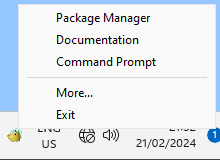
\includegraphics[width=4cm]{tray-menu}
\smallskip

\noindent Der Eintrag \enquote{More\ldots} erläutert, wie Sie dieses Menü anpassen können.

%\subsection{\ISO- (oder \DVD-) Installationen}
%\label{sec:isoinstall}
%
%Wenn Sie ihre Installation nicht aktualisieren oder anpassen müssen, kann die Erstellung einer ISO Datei oder DVD Ihrer Installation vorteilhaft sein, denn:
%
%\begin{itemize}
%\item Das Kopieren einer ISO-Datei zwischen zwei Computern ist deutlich schneller als eine erneute \TL{} Installation,
%\item Eine ISO Installation ist von den anderen Dateisystemen des jeweils genutzten Rechners unabhängig,
%\item Virtuelle Maschinen können ein ISO-Image leicht einbinden.
%\end{itemize} \enlargethispage{1cm}
%
%Natürlich können Sie auch ein ISO-Image auf DVD brennen, wenn dies für Sie vorteilhaft ist.
%
%Desktop \GNU/Linux/Unix Systeme, inklusive \macOS, können ISO-Images seit langem problemlos einbinden. Windows 8 ist die erste Windows-Version, die dies auch mit Bordmitteln kann. 
%
%Wenn man eine ISO-Installation vorbereitet, ist es am besten, das Verzeichnis für das Jahr wegzulassen und und \filename{texmf-local} auf der gleichen Ebene wie (\filename{texmf-dist}, \filename{texmf-var}, etc.) zu haben. Dies kann man im normalen Installationsprogramm einstellen.
%
%Um ein physikalisches Installationsmedium zu erhalten, kann man das ISO-Image auf DVD brennen.
%
%Für die Windows System-Integration können Sie die \filename{w32client} einbeziehen, die in Kapitel~\ref{sec:sharedinstall} und unter \url{https://tug.org/texlive/w32client.html} beschrieben sind, und die mit einem ISO-Image genauso funktionieren wie in einer Netzwerkinstallation.
%
%Unter \macOS lassen sich TeXShop und \TeX{}works nutzen, wenn ein symbolischer Link\filename{/usr/texbin} auf das entsprechende Verzeichnis zeigt, wie z.\,B. 
%\begin{verbatim}
%sudo ln -s /Volumes/MyTeXLive/bin/universal-darwin /usr/texbin
%\end{verbatim}

\chapter{tlmgr: Installation verwalten}\label{sec:tlmgr}

\begin{figure}[tb]
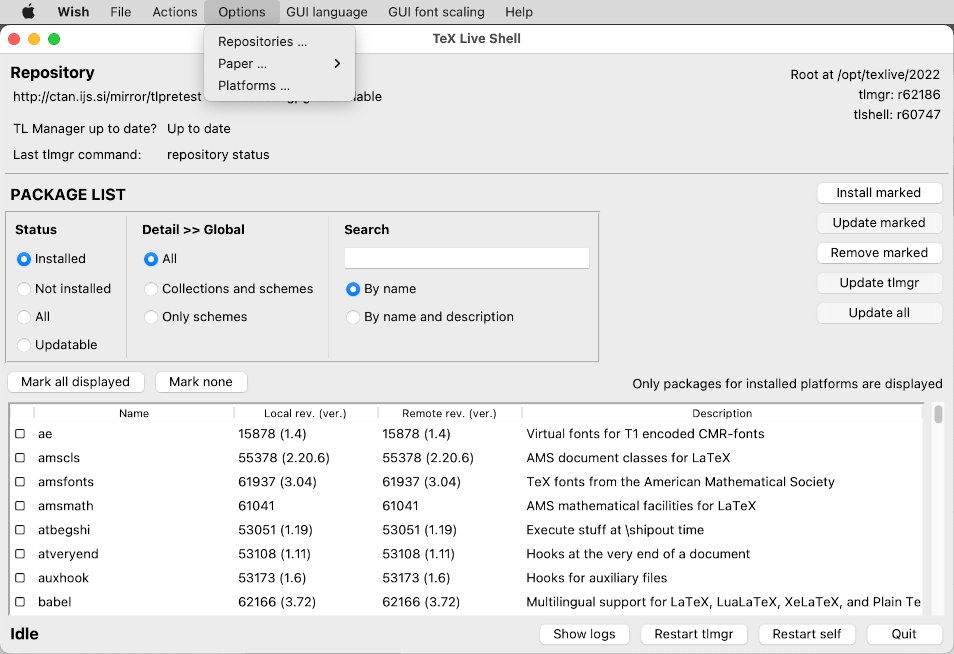
\includegraphics[width=\linewidth]{tlshell-macos}
\caption{\prog{tlshell} GUI, mit dem Auswahlmenü (Mac OS X)}
\label{fig:tlshell}
\end{figure}

\begin{figure}[tb]
\includegraphics[width=\linewidth]{tlcockpit-packages}
\caption{\prog{tlcockpit} GUI für \prog{tlmgr}}
\label{fig:tlcockpit}
\end{figure}

\begin{figure}[tb]
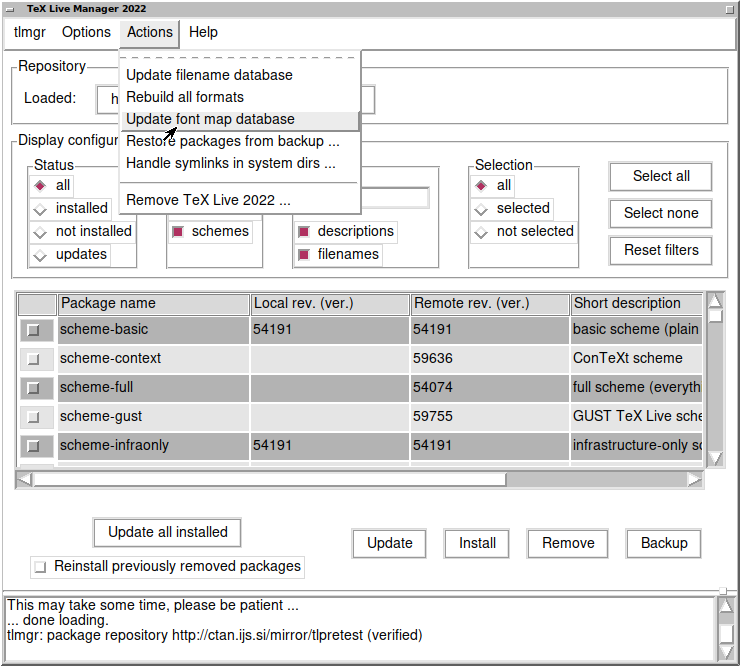
\includegraphics[width=\linewidth]{tlmgr-gui}
\caption{Legacy-\prog{tlmgr} im GUI-Modus. Hauptfenster nach dem Klick auf \enquote{Load}.}\label{fig:tlmgr-gui}
\end{figure}

\begin{figure}[h]
	\centering
    \includegraphics[width=0.65\linewidth]{tlmgr-general-options}
    \caption{\texttt{tlmgr} im GUI-Modus: Allgemeine Optionen}
    \label{fig:tlmgr-general-options}
\end{figure}

\begin{figure}[h]
\centering
\includegraphics[width=0.65\linewidth]{tlmgr-paper-options}
    \caption{\texttt{tlmgr} im GUI-Modus: Optionen zur Papiergröße.}
    \label{fig:tlmgr-paper-options}
\end{figure}

Bei der Installation von \TL wird auch das Programm~\prog{tlmgr} installiert, mit dem Sie anschließend Ihr \TL-System verwalten können. Die hierfür bisher verwendeten Programme~\prog{updmap}, \prog{fmtutil} und \prog{texconfig} sind zwar noch vorhanden, aber inzwischen ist \prog{tlmgr} die vorgesehene Oberfläche zur Konfiguration von \TL. Mit \prog{tlmgr} können Sie folgende Aufgaben erledigen:

\begin{itemize} % @@@@@
\item Verfügbare Schemata, Collections und Pakete installieren, aktualisieren, wieder
     herstellen, sichern, deinstallieren, auf Wunsch mit Berücksichtigung von Paketabhängigkeiten.
\item Suchen nach Paketen.
\item Anzeigen der Systeme, unter denen \TL läuft; (de)installieren von Binaries für weitere Systeme.
\item Anpassen der Installation, wie Ändern der Papiergröße oder des Quellverzeichnisses für Komponenten
 (s.\,Kapitel~\ref{sec:location}).
\end{itemize}

\prog{tlmgr} hat die vollständige Funktionalität von \prog{texconfig}, das aber noch mit ausgeliefert wird. Wir empfehlen aber, \prog{tlmgr} zu nutzen.

\section{Aktuelle \texttt{GUI}-Interfaces für \cmdname{tlmgr}}

\TL{} enthält mehrere GUIs für \prog{tlmgr}. Abbildung~\ref{fig:tlshell} zeigt \cmdname{tlshell},
das in Tcl/Tk geschrieben wurde und unter Windows und 
and Mac OS X ohne zusätzliche Software funktioniert. Abbildung~\ref{fig:tlcockpit} zeigt \prog{tlcockpit}, das Java version~8 oder höher sowie JavaFX benötigt. Beide Programme sind separate Pakete.

\prog{tlmgr} selbst kann im GUI-Modus laufen, siehe Abbildung
~\ref{fig:tlmgr-gui}):

\begin{alltt}
> \Ucom{tlmgr -gui}
\end{alltt}

Diese Benutzeroberfläche benötigt Perl/Tk, das nicht Teil der \TL\ Perl Distribution unter Windows ist.

\section{Beispiel zur Verwendung von tlmgr über die Kommandozeile}


Nachdem Sie \TL\ installiert haben, können Sie Ihr \TL-System auf den
neuesten Stand aktualisieren:
\begin{alltt}
> \Ucom{tlmgr update -all}
\end{alltt}
Falls Sie vorher wissen möchten, was ein Update alles aktualisieren würde, können Sie zunächst
\begin{alltt}
> \Ucom{tlmgr update -all -dry-run}
\end{alltt}
oder (weniger ausführlich)
\begin{alltt}
> \Ucom{tlmgr update -list}
\end{alltt}
verwenden.

Das folgende Beispiel demonstriert, wie die Collection für \XeTeX\ installiert
wird, wobei sich die Installationsdateien in einem lokalen Verzeichnis
befinden:
 
\begin{alltt}
\Ucom{tlmgr -repository /local/mirror/tlnet install collection-xetex}
\end{alltt}
Dies liefert die eine  Ausgabe wie die folgende:

\begin{alltt}\small
install: collection-xetex
install: arabxetex
...
install: xetex
install: xetexconfig
install: xetex.i386-linux
running post install action for xetex
install: xetex-def
...
running mktexlsr
mktexlsr: Updating /usr/local/texlive/2023/texmf-dist/ls-R...
...
running fmtutil-sys --missing
...
Transcript written on xelatex.log.
fmtutil: /usr/local/texlive/2023/texmf-var/web2c/xetex/xelatex.fmt installed.
\end{alltt}

Wie man sieht, beachtet \prog{tlmgr} die Abhängigkeiten von Paketen und installiert im obigen Beispiel von \XeTeX{} benötigte Komponenten nach. Weiterhin werden automatisch im Anschluss die Dateilisten der Verzeichnisbäume aktualisiert und fehlende Formate generiert.

Informationen zu einem Paket (oder einer Collection oder einem Schema) anzeigen:

\begin{alltt}
Ucom{tlmgr show collection-latexextra}
\end{alltt}

Hier erhält man folgende Ausgabe:

\begin{verbatim}
package:    collection-latexextra
category:   Collection
shortdesc:  LaTeX supplementary packages
longdesc:   A very large collection of add-on packages for LaTeX.
installed:  Yes
revision:   46963
sizes:      657941k
\end{verbatim}

\noindent Die komplette Dokumentation finden Sie unter \url{https://tug.org/texlive/tlmgr.html}
oder mit \texttt{tlmgr -help}.

\chapter{Hinweise zu Windows}
\label{sec:windows}


\section{Windows-spezifische Dinge}
\label{sec:winfeatures}

Unter Windows kümmert sich das Installationsprogramm auch um folgende Dinge:

\begin{description}
\item[Menüs und Verknüpfungen.] Im Startmenü wird ein Menü \enquote{\TL} hinzu gefügt. Hier sind Einträge für
  die grafischen Anwendungen (\prog{tlmgr}, \prog{texdoctk} 
  und einige Verknüpfungen zur Dokumentation vorhanden. 
\item[Automatisches Setzen der Umgebungsvariablen.] Hierdurch ist das Setzen dieser Variablen
  von Hand überflüssig geworden.
\item[Uninstaller.] Es wird ein Eintrag zum Entfernen von \TL in der Systemsteuerung im Punkt \enquote{Software} angelegt, bei Einzelinstallationen auch ein entsprechender Menüeintrag im Startmenü.
  Alternativ können Sie \TL über die GUI \TeX\ Live Manager deinstallieren.
\item[Dateiverknüpfungen] Wenn diese Option aktiviert wird, werden \prog{TeXworks} und \prog{Dviout}
  entweder die Standard-Programme für die entsprechenden Dateitypen oder erhalten einen Eintrag im \enquote{Öffnen mit} Dialog. \enlargethispage{1.5cm}
\item[Bitmap nach eps Konverter] Verschiedene Bitmap-Formate erhalten einen Eintrag \cmdname{bitmap2eps} in Ihr \enquote{Öffnen mit} Menü. Bitmap2eps ist ein einfaches Skript, das im Hintergrund \cmdname{sam2p} oder \cmdname{bmeps} aufruft. 
\item[Automatische Pfad-Anpassung] Erfordert keine manuellen Anpassungen.
\item[Schreibschutz] Admin-gestützte Installationen sind gegen User-Zugriff schreibgeschützt. 
\end{description}


\section{Zusätzlich enthaltene Programme unter Windows}

Zusätzlich werden unter Windows einige Programme installiert:

\begin{description}
\item[Perl und Ghostscript.] Da Perl und Ghostscript für \TL sehr wichtig sind, werden diese   unter Windows mitgeliefert und intern von \TL benutzt. Die in \TL enthaltenen Programme, die diese Komponenten benötigen, \enquote{wissen} wo sich diese befinden, ohne dass diese im System durch  Umgebungsvariablen oder Einträge in der Registry sichtbar sind. Es handelt sich um für \TL abgespeckte Versionen, die zu keinen Konflikten mit eventuell bereits vorhandenen Installationen von Perl und Ghostscript führen sollten.

\item[PS\_View.] Weiterhin wird PS\_View installiert, ein neuer PostScript- und PDF-Viewer, der Freie Software ist, siehe Abbildung~\ref{fig:psview}.

\begin{figure}[tb]
\begin{center}
\includegraphics[width=.6\linewidth]{psview}
\caption{PS\_View, sogar sehr extreme Vergrößerungen sind möglich.}\label{fig:psview}
\end{center}
\end{figure}

\item[dviout] Weiterhin wird \prog{dviout}, ein \acro{DVI}-Viewer installiert.
Wenn Sie am Anfang Dokumente mit \cmdname{dviout} anschauen, werden häufig noch Fonts generiert, da keine fertigen Fontdateien für den Bildschirm mitgeliefert werden. Je mehr Fonts generiert wurden, desto seltener müssen Schriften nachgeneriert werden, so dass dieser Effekt nach einiger Zeit nur noch selten auftreten wird. Weitere Informationen finden Sie in der (sehr guten) Online-Hilfe. \enlargethispage{1cm}

\item[TeXworks] \TeX{}works ist eine Oberfläche für \TeX\ mit Editor und
   integriertem \acro{PDF}-Viewer.

\item[Tools für die Kommandozeile.] Für einige unter Linux/Unix üblicherweise vorhandene Programme werden Portierungen für Windows mitgeliefert. Dies sind z.\,B. \cmdname{gzip}, \cmdname{zip}, \cmdname{unzip} und einige Programme für die Kommandozeile aus der
   \cmdname{xpdf}-Suite, wie \cmdname{pdfinfo}, und \cmdname{pdffonts}.  (Vom
   \cmdname{xpdf}-Viewer selbst gibt es keine Version für Windows, aber der empfehlenswerte 
   Sumatra \acro{PDF}-Viewer basiert auf \cmdname{xpdf}:
   \url{https:///sumatrapdfreader.org}.)
 \item[\texttt{fc-cache}, \texttt{fc-list} etc.] dienen \XeTeX{} zur effizienteren Benutzung von Schriften. Mit \prog{fc-list} können Sie die Namen der
   verfügbaren Schriften anzeigen, die Sie dann unter \XeTeX\ mit dem
   Kommando \texttt{font} benutzen können. Mit \prog{fc-cache} kann die Liste
   der verfügbaren Schriften aktualisiert werden.
\end{description}


\section{Nutzerprofile unter Windows}
\label{sec:winhome}

Das Gegenstück von Windows zum HOME-Verzeichnis unter Unix ist das
Verzeichnis \verb|%USERPROFILE%|, ab Windows Vista liegt es meist in \verb|C:\Users\<username>|.

In der Datei  \filename{texmf.cnf} und in \KPS{} allgemein wird \verb|~| 
sowohl unter Unix und Windows korrekt aufgelöst.

\section{Die Windows-Registry}
\label{sec:registry}

Windows verwaltet fast all seine Konfigurationseinstellungen in der Registry. Diese besteht aus einem hierarchisch aufgebauten Baum von Schlüsseln, wobei mehrere dieser Registry-Bäume existieren. Die wichtigsten sind \path{HKEY_CURRENT_USER} und \path{HKEY_LOCAL_MACHINE}, oft abgekürzt als \path{HKCU} bzw.\ \path{HKLM}. Der \path{HKCU}-Teil der Registry wird im Home-Verzeichnis des Benutzers gespeichert (siehe Kapitel~\ref{sec:winhome}). \path{HKLM} liegt im
Normalfall in einem Unterverzeichnis des Windows-Verzeichnisses.

In einigen Fällen sind Systeminformationen aus Umgebungsvariablen ersichtlich, in vielen anderen Fällen liegen diese Informationen aber in der Registry.

\section{Windows Zugriffskontrolle}
\label{sec:winpermissions}

In neueren Versionen von Windows wird zwischen normalen Benutzern und Administratoren unterschieden, wobei nur letztere freien Zugang auf alle Teile des Betriebsystems haben. 
Im Gegensatz zu Unix ist es in der Praxis allerdings häufig so, dass Benutzer zur Klasse der Administratoren
gehören und daher doch alle Freiheiten haben. 
Trotzdem haben wir einigen Aufwand getrieben, damit \TL auch unter Windows ohne Administrator-Rechte
installiert werden kann.

Wenn das \TL Installationsprogramm mit Administrator-Rechten gestartet wird, gibt es eine Option für die Installation für alle Benutzer des Systems, d.\,h. Verknüpfungen, Menüs und Systemeinträge werden für alle Nutzer angelegt. 
Ansonsten werden diese nur für den aktuellen Benutzer angelegt.

Unabhängig davon wird grundsätzlich angenommen, dass das Wurzelverzeichnis
von \TL unter \verb|%SystemDrive%| liegen soll. Allerdings testet das
Installationsprogramm, ob dieses Verzeichnis für den aktuellen Benutzer
schreibbar ist.

Ein Problem entsteht, wenn \TL ohne Administrator-Rechte installiert
wird und sich bereits ein \TeX{}-System im systemweiten Suchpfad
befindet. Windows benutzt zuerst den Suchpfad des Systems, erst dann
den spezifischen Suchpfad des Nutzers, sodass hier immer zuerst
das alte \TeX-System gefunden wird. Der Workaround in diesem Fall ist, eine Verknüpfung zu einer Eingabeaufforderung zu erzeugen, bei der das \TL Programmverzeichnis \textbf{vor} den Standard\-such\-pfad
geschrieben wird. Dies bedeutet aber, dass das neue \TL in diesem Fall nur in einer
Eingabeaufforderung verfügbar ist, die über genau diese Verknüpfung gestartet
wird. Die Verknüpfung für \TeX{}works (falls Sie dieses installieren)
fügt ebenfalls automatisch \TL{} am Anfang des Suchpfades ein, so dass
es direkt benutzbar ist.

Es gibt es noch einen weiteren Fallstrick. 
Selbst wenn Sie als Administrator angemeldet sind, müssen Sie bestimmte Programme trotzdem explizit
mit Administratorrechten starten. 
Insofern ist es tatsächlich nicht sehr sinnvoll, sich als Administrator anzumelden. 
Klicken Sie stattdessen auf das gewünschte Programm (bzw. die gewünschte Verknüpfung) mit der
rechten Maustaste, damit Sie die Option \enquote{Als Administrator ausführen...} erhalten, um dieses mit Administratorrechten auszuführen.

\section{Erhöhen des maximal verfügbaren Speichers unter Windows und Cygwin}
\label{sec:cygwin-maxmem}

Unter Windows und Cygwin (s. Kapitel \ref{sec:cygwin} für die Installation unter
Cygwin) kann es vorkommen, dass der den in \TL\ enthaltenen Programmen zur
Verfügung gestellte Speicher nicht ausreicht. Dies kann z.\,B. passieren, wenn 
ein Dokument mit umfangreichen Schriften mit Lua\TeX\ übersetzt wird.

Für Cygwin ist die Erhöhung des Maximalspeichers im Cygwin-Hanbuch beschrieben
(\url{https://www.cygwin.com/cygwin-ug-net/setup-maxmem.html}).

Unter Windows können Sie eine Datei \code{moremem.reg} mit folgenden vier
Zeilen anlegen:

\begin{verbatim}
Windows Registry Editor Version 5.00

[HKEY_LOCAL_MACHINE\Software\Cygwin]
"heap_chunk_in_mb"=dword:ffffff00
\end{verbatim}

Führen Sie dann als Administrator \code{regedit /s moremem.reg} aus.
(Falls der zur Verfügung stehende Speicher nur für den aktuellen Nutzer
erhöht werden soll, verwenden Sie stattdessen einfach \code{HKEY\_CURRENT\_USER}).

\chapter{Anleitung zum Web2C-System}

Web2C besteht aus einer Reihe von Programmen, die zusammen ein komplettes
\TeX-System darstellen. Dazu gehören natürlich \TeX, \MF, \MP, {\BibTeX} usw.

Die erste Implementierung eines \TeX-Systems in der Programmiersprache C stammt von Tomas~Rokicki und datiert zurück in das Jahr 1987. Rokicki benutzte als Basis sog. Change-Files unter \acro{UNIX}, die ursprünglich von Howard~Trickey und Pavel~Curtis entwickelt wurden. Tim~Morgan hat dieses System, für das der Name  Web-to-C\@ eingeführt wurde, gepflegt. 1990 hat Karl~Berry mit Unterstützung vieler Helfer die Weiterentwicklung übernommen und 1997 an Olaf~Weber weitergegeben, der es 2006 wieder an Karl zurückgab.

Web2C läuft unter \acro{UNIX}, Windows, \macOS{}
und auf weiteren Betriebssystemen. Es benutzt die
Original-Quelldateien von Donald E.~Knuth und weitere in der
Sprache \texttt{WEB} entwickelte Programme als Basis und übersetzt diese
in C-Quell-Code. Darüber hinaus bietet das System viele Makros und
Funktionen zur Nutzung der originalen \TeX-Software. Hier eine
Liste der Basisprogramme eines \TeX-Systems:

\begin{description}
\item[bibtex]   Verwalten von Bibliographien
\item[dvicopy]  Umwandeln von virtuellen Zeichensätzen in DVI-Dateien
\item[dvitomp]  DVI-nach-MPX-Konverter (\MP-Bilder)
\item[dvitype]  Textanzeige aus DVI-Dateien
\item[gftodvi]  Erzeugen von Prüfausgaben für Zeichensätze
\item[gftopk]   Packen von Zeichensätzen
\item[gftype]   Anzeige von Zeichensätzen als ASCII-Graphik
\item[mf]       Zeichensatzerzeugung
\item[mft]      formatierte Ausgabe von \MF-Quellen
\item[mpost]    \MF-ähnliches Grafikprogramm
\item[patgen]   Erzeugen von Trennmustern
\item[pktogf]   Entpacken von Zeichensätzen
\item[pktype]   Anzeige gepackter Zeichensätze
\item[pltotf]   Umwandeln von Property-Listen in \file{.tfm}-Dateien
\item[pooltype] Anzeige der Bildschirmtexte eines WEB-Programms
\item[tangle]   Konverter {\web} nach Pascal
\item[tex]      \TeX-Programm
\item[tftopl]   Umwandeln einer \file{.tfm}-Datei in eine Property-Liste
\item[vftovp]   Umwandeln eines virtuellen Zeichensatzes in eine Property-Liste
\item[vptovf]   Umwandeln einer Property-Liste in einen virtuellen Zeichensatz
\item[weave]    \web-Code als \TeX-Dokumentation
\end{description}

Die genaue Funktionsweise und die möglichen Parameter sind der
Beschreibung der jeweiligen Pakete bzw.\ der Web2C-Dokumentation zu entnehmen.
Trotzdem wird ein Überblick über Zusammenspiel und Funktionsweise der
Web2C-Programme Ihnen sicherlich helfen, besser mit dem System zurechtzukommen.

Zunächst verstehen alle Programme die grundlegenden Parameter der
\acro{GNU}-Software:

\begin{description}
\item[\texttt{-{}-help}] kurzer Hilfstext
\item[\texttt{-{}-verbose}] ausführliche Ausgaben beim Programmablauf
\item[\texttt{-{}-version}] nur Ausgabe der Versionsnummer 
\end{description}

\noindent Die Programme des Web2C-Systems benutzen zur Lokalisierung der benötigten
Dateien im Dateisystem die \KPS-Bibliothek (\url{https://tug.org/kpathsea}). Diese Bibliothek optimiert und beschleunigt den Suchprozess im Dateisystem. Ihre Arbeitsweise wird durch
einige Umgebungsvariablen und eine Kon"-fi"-gu"-ra"-tions"-da"-tei gesteuert.
Web2C kann mehr als einen Dateibaum gleichzeitig verwalten und ermöglicht
somit die schon beschriebene \TL-Installation unter Verwendung der
{\DVD} mit der Ablage modifizierter Konfigurationsdateien
und zusätzlicher Zeichensätze in einem zweiten Dateibaum. Die Suche
nach Dateien wird durch die Analyse der Datei \file{ls-R} beschleunigt,
die in jedem Wurzelverzeichnis eines \TeX-Dateibaums vorhanden ist.
Sie enthält für jede Datei die genaue Position im Dateibaum relativ
zum Wurzelverzeichnis.


\section{Dateisuche mit der Kpathsea-Bibliothek}
\label{sec:kpathsea}

Wir beschreiben zunächst den grundlegenden Suchmechanismus der \KPS-Bibliothek.

Ein \textit{Suchpfad} ist eine durch Kommata oder Semikola getrennte Liste von
\textit{Pfadkomponenten}, die üblicherweise Verzeichnisnamen darstellen.
Ein Suchpfad kann sich aus vielen Komponenten zusammensetzen. Die Suche nach
einer Datei \samp{my-file} über den Suchpfad \samp{.:/dir} bewirkt, dass
{\KPS} jede Komponente nacheinander überprüft, also zunächst
\samp{./my-file} und dann \samp{/dir/my-file}. Als Ergebnis wird entweder die
erste gefundene Datei oder eine Liste aller passenden Dateien geliefert.

Um auf allen Dateisystemen effizient arbeiten zu können, verwendet {\KPS} ggf. andere Datei-/""Verzeich"-nis-Separatoren als \samp{:} und \samp{/}.

Beim Überprüfen einer Pfadkomponente \var{p} überprüft {\KPS} zunächst,
ob eine Dateinamen"=Datenbank (siehe auch Dateinamen"=Datenbank auf
Seite~\pageref{sec:filename-database}) für die Pfadkomponente zuständig ist,
d.\,h. beispielsweise steht die Datenbank in einem Verzeichnis, das im Pfad
vor der zu überprüfenden Komponente \var{p} steht. In diesem Fall wird
zur Bestimmung der Position der gesuchten Datei die Datenbank herangezogen.

%Nur wenn keine passende Datenbank existiert oder wenn die Datei nicht
%in der Datenbank gefunden wird, durchsucht {\KPS} das Dateisystem. Diese
%zeitaufwändige Suche kann über die Spezifikation der Pfadkomponente \var{p}
%mit dem Präfix \samp{!!}\ unterbunden werden. Zur Suche erzeugt {\KPS} eine
%Liste der Verzeichnisse, die im Pfadelement enthalten sind, und durchsucht
%jedes dieser Verzeichnisse nach der gesuchten Datei.
%
%Für Dateien kann auch ein Schalter \samp{file~must~exist} gesetzt werden (\enquote{Datei muss vorhanden sein}). Wenn dieser Schalter nicht gesetzt ist und beispielsweise über das \TeX-Kommando \code{openin} eine VF-Datei wie \file{cmr10.vf} gelesen werden soll, wäre es falsch, nach dieser Datei zu suchen, weil es sie gar
%nicht gibt. Speziell für neu installierte VF-Dateien sollten Sie also unbedingt die Dateinamen"=Datenbank (\cmdname{ls-R}) aktualisieren, weil die Dateien sonst nicht gelesen werden und kein Fehler angezeigt wird. Dieser Vorgang wiederholt sich für jede Komponente eines Suchpfades: zunächst wird die Datenbank
%überprüft, danach ggf. das Dateisystem. Wird die Datei gefunden,
%stoppt die Suche (normalerweise) und als Ergebnis wird der komplette Pfad zur
%gesuchten Datei ausgegeben.

Außer Verzeichnisnamen dürfen Pfadkomponenten für {\KPS} folgende
Elemente enthalten: (verschachtelte) Vorgaben, Umgebungsvariablen,
Werte aus der Konfigurationsdatei, Home-Verzeichnisse von
Benutzern und Startverzeichnisse für eine rekursive Suche. Diese
Elemente werden vor einer Dateisuche von {\KPS} in gewöhnliche
Verzeichnis- oder Dateinamen expandiert. Diese Expansion wird in
den folgenden Abschnitten erklärt, und zwar genau in der
Reihenfolge, wie die Elemente auch von {\KPS} bearbeitet werden.

Beachten Sie, dass {\KPS} bei absoluten und explizit relativen Komponenten,
d.\,h. wenn die Komponente mit den Zeichen \samp{/}, \samp{./} oder
\samp{../} beginnt, nur überprüft, ob die Datei existiert.

%\begin{figure*}[tp]
%\verbatiminput{../texlive-common/examples/ex5.tex}
%\setlength{\abovecaptionskip}{0pt}
%  \caption{An illustrative configuration file sample}
%  \label{fig:config-sample}
%\end{figure*} XXXXX

\subsection{Bestandteile von Pfadkomponenten}
\label{sec:path-expansion}


Ein Suchpfad kann aus vielen verschiedenen Bestandteilen aufgebaut werden.
Dies sind in der Reihenfolge, wie {\KPS} sie auswertet:

\begin{enumerate}
\item
  eine benutzerdefinierte Umgebungsvariable, z.\,B. \envname{TEXINPUTS}:
  Wird an den Inhalt der Variablen ein Punkt und ein Programmname angehängt, wie
  beispielsweise bei \envname{TEXINPUTS.latex}, hat diese Form Vorrang
  vor den \enquote{gewöhnlichen} Variablen.
\item
  Einträge aus programmspezifischen Konfigurationsdateien,
  beispielsweise zum Programm \code{dvips} eine Zeile \code{S /a:/b}
  in der Konfigurationsdatei \file{config.ps}
\item
  Einträge aus der \KPS-Konfigurationsdatei \file{texmf.cnf}, wie 
  zum Beispiel \code{TEXINPUTS=/c:/d} (siehe folgenden Text).
\item
  Einstellung beim Übersetzen der Programme.
\end{enumerate}

\noindent Unter Verwendung der Parameter zur Fehlersuche können Sie sich diese
Werte für einen Suchpfad auch anzeigen lassen. (Siehe dazu das Kapitel
\enquote{Fehlersuche} auf Seite~\pageref{sec:debugging}.)

\subsection{Konfigurationsdateien}

Die \KPS-Bibliothek liest zur Laufzeit die \emph{Konfigurationsdateien} mit den Namen \file{.../2022/texmf.cnf}. Sollten Sie Anpassungen an den Standardvorgaben vornehmen \textit{müssen}, ist dies der richtige Ort. 

Die Haupt-Konfigurationsdatei befindet sich in \file{.../2022/texmf-dist/web2c/texmf.cnf}. Diese Datei sollten Sie nicht anpassen, da Ihre Anpassungen beim nächsten Update überschrieben werden.

Im Folgenden wird die Syntax der Datei \file{texmf.cnf} angegeben. Konsultieren Sie zum besseren Verständnis beim Lesen die auf der DVD enthaltene Konfigurationsdatei.

\begin{itemize}
\item
  Kommentare beginnen mit einem \code{\%} und erstrecken sich bis zum
  Zeilenende.
\item
  Leerzeilen werden überlesen.
\item
  Ein \samp{\bs} am Zeilenende fasst die aktuelle mit der folgenden Zeile
  zusammen. Leerraum in der Folgezeile wird \emph{nicht} überlesen.
\item
  Sonstige Zeilen haben den folgenden Aufbau:

\begin{alltt}
  \var{Variable}[.\var{Programmname}] [=] \var{Wert}
\end{alltt}%

  Das Zeichen ">="< und umgebender Leerraum dürfen entfallen.
\item
  Der Name von \var{Variable} kann alle Zeichen außer Leerzeichen,
  \samp{=} und \samp{.} enthalten. Verwenden Sie am besten nur die Zeichen
  \samp{A-Za-z\_}.
\item
  Wenn das Suffix ">\code{.\var{Programmname}}"< angegeben wird, gilt die
  Variable nur für das entsprechende Programm ">\var{Programmname}"< oder
  ">\code{\var{Programmname}.exe}"<. Auf diese Weise können
  beispielsweise verschiedene
  \TeX-Formate mit unterschiedlichen Suchpfaden arbeiten.
\item
  \texttt{\var{Wert}} darf alle Zeichen außer \texttt{\%} und \texttt{@}
  enthalten.
  Die Einschränkung der Werte auf bestimmte Programme über ein Suffix
  ist nicht zulässig. Ein \samp{;} in \texttt{\var{Wert}} wird unter
  \acro{UNIX} in \samp{:} umgewandelt. Dadurch ist die Verwendung der gleichen
  Konfigurationsdateien für \acro{UNIX} und \acro{DOS}/""Windows"=Systeme möglich.
\item
  Die Definitionen werden komplett eingelesen, bevor eine Expansion
  stattfindet. Dadurch können Sie die Variable schon vor Ihrer Definition
  referieren.
\end{itemize}

Der Ausschnitt einer Konfigurationsdatei demonstriert diese
Möglichkeiten:

\verbatiminput{../texlive-common/examples/ex5.tex}

%Betrachten Sie Abbildung~\ref{fig:config-sample}.

\subsection{Expansion von Pfadkomponenten}

{\KPS} verwendet in Suchpfaden ähnliche Zeichen und Konstrukte wie
\acro{UNIX}-Shells. Beispielsweise wird die Definition
\verb|~$USER/{foo,bar}//baz| in alle Unterverzeichnisse von \file{foo} und
\file{bar} unterhalb vom Home-Verzeichnis von \dirname{\$USER} expandiert,
die eine Datei oder ein Unterverzeichnis namens \file{baz} enthalten. Der
Expansionsmechanismus wird im Folgenden erklärt.

\subsection{Expansion der Voreinstellungen}\label{sec:default-expansion}

Wenn der Suchpfad mit der höchsten Priorität (siehe hierzu \enquote{Bestandteile von
Pfadkomponenten} auf Seite~\pageref{sec:path-expansion}) einen zusätzlichen (vorangestellten, nachgestellten oder verdoppelten) Doppelpunkt enthält, wird an dieser Stelle der Suchpfad eingefügt, der als nächstes in der
Hierarchie folgt. Auch bei diesem gilt dieselbe Regel. Wenn beispielsweise
die Umgebungsvariable


\begin{alltt}
> \Ucom{setenv TEXINPUTS /home/karl:}
\end{alltt}

gesetzt wird (hier: C-Shell) und in \file{texmf.cnf} die Variable
\code{TEXINPUTS} folgenden Wert erhält

\begin{alltt}
  .:\$TEXMF//tex
\end{alltt}

dann lautet der Suchpfad schließlich:

\begin{alltt}
  /home/karl:.:\$TEXMF//tex
\end{alltt}

Da es sinnlos wäre, denselben Pfad mehrfach einzufügen, wird die Ersetzung
nur einmal vorgenommen, und zwar in der Reihenfolge vorne, hinten und
Mitte. Mehrfach verdoppelte Doppelpunkte bleiben unverändert.

\subsection{Expansion geschweifter Klammern}

Die Expansion geschweifter Klammern ist zur Definition mehrerer \TeX-Hierarchien sehr nützlich. Beispielsweise wird |v{a,b}w| zu |vaw:vbw|. Verschachtelungen sind dabei erlaubt. Diese Technik wird dazu benutzt, durch eine Zuweisung an
\code{\$TEXMF} verschiedene \TeX-Hierarchien einzuführen. Als Beispiel finden Sie in \file{texmf.cnf} folgende Definition (etwas gekürzt, tatsächlich ist es etwas komplexer):

\begin{verbatim}
  TEXMF = {$TEXMFVAR,$TEXMFHOME,!!$TEXMFLOCAL,!!$TEXMFDIST}
\end{verbatim}

Eine Anwendung wie

\begin{verbatim}
  TEXINPUTS = .;$TEXMF/tex//
\end{verbatim}

führt dann dazu, dass erst im aktuellen Verzeichnis gesucht wird, dann
im gesamten Dateibaum \code{\$TEXMFVAR/tex}, \code{\$TEXMFHOME/tex}, \code{\$TEXMFLOCAL/tex} und schließlich im gesamten Dateibaum \dirname{\$TEXMFDIST/tex} (die letzten beiden nur in der Datenbank \file{ls-R}) durchsucht wird. Dadurch kann man bequem zwei parallel installierte \TeX-Hierarchien durchsuchen, beispielsweise eine unveränderliche auf \acro{CDROM}/{\DVD} und eine dynamisch angepasste auf Festplatte, in der neue Programmversionen und zusätzliche Zeichensätze installiert werden. Durch die Verwendung der Variablen \code{\$TEXMF} in allen Definitionen wird grundsätzlich zuerst der neuere Dateibaum durchsucht.


\subsection{Expansion von Unterverzeichnissen}\label{sec:subdirectory-expansion}

Zwei oder mehrere aufeinanderfolgende Schrägstriche (\texttt{//}) in einer Pfadkomponente, die auf einen Verzeichnisnamen \var{d} folgen, werden expandiert zu allen Unterverzeichnissen von \var{d}. Dieser Vorgang findet rekursiv statt, wobei erst alle Verzeichnisse auf einer Ebene bearbeitet werden, dann deren Unterverzeichnisse, usw. Auf den jeweiligen Ebenen ist nicht beeinflussbar, in welcher Reihenfolge die Unterverzeichnisse bearbeitet werden.

Wenn nach den Schrägstrichen Namen angegeben werden, dann werden nur
Unterverzeichnisse mit passenden Namen in die Suche einbezogen. Beispielsweise wird \code{/a//b} in die Pfade \file{/a/1/b}, \file{/a/2/b}, \file{/a/1/1/b} usw. expandiert, aber nicht zu \file{/a/b/c} oder \file{/a/1}. (Jeweils vorausgesetzt, dass die Verzeichnisse existieren.)

Mehrere \code{//}-Konstruktionen innerhalb einer Pfadkomponente
sind zulässig, allerdings nicht am Pfadanfang.


\subsection{Liste der Sonderzeichen und ihre Bedeutung: eine Zusammenfassung}


Die folgende Zusammenfassung fasst alle Sonderzeichen zusammen, die in den
\KPS"=Konfigurationsdateien auftreten können:

% ++++++++++++++++++++++++ %xxxx todo
\newcommand{\CODE}[1]{\makebox[3em][l]{\code{#1}}}
% ++++++++++++++++++++++++

\begin{description}
\item[\CODE{:}]  Trennzeichen für Pfadkomponenten; als erstes
                    oder letztes Zeichen im Pfad bewirkt es die
                    Expansion der Voreinstellungen.
\item[\CODE{;}]  Trennzeichen für Pfadkomponenten für andere
                    Rechnerplattformen als \acro{UNIX} (Verwendung wie
      ">\code{:}"<)
\item[\CODE{\$}]    Expansion von Variableninhalten
\item[\CODE{\string~}]   Home-Verzeichnis eines Benutzers (Tilde)
\item[\CODE{\char`\{...\char`\}}] Expansion geschweifter Klammern:
                    beispielsweise wird |a{1,2}b| zu |a1b:a2b|.
\item[\CODE{//}]    Expansion von Unterverzeichnissen: tritt niemals
                    am Anfang einer Pfadkomponente auf.
\item[\CODE{\%}]    Kommentar
\item[\CODE{\bs}]   Konkatenation mit Folgezeile(n)
\item[\CODE{!!}]    Einschränkung der Suche \emph{ausschließlich} auf die
                    Dateinamen"=Datenbank: Das Dateisystem wird \emph{nicht}
                    durchsucht!
\end{description}



\section{Dateinamen-Datenbanken}\label{sec:filename-database}

\KPS unternimmt etliche Anstrengungen, um den Zugriff auf Festplatte und
DVD zur Suche nach Dateien zu reduzieren. Auf \TeX-Systemen mit vielen Unterverzeichnissen kann die Suche in jedem möglichen Verzeichnis nach einer bestimmten Datei eine lange Zeit in Anspruch nehmen, besonders wenn einige Hundert Zeichensatzverzeichnisse durchforstet werden müssen. Um dieses Problem abzumildern, benutzt {\KPS} eine Art Datenbankdatei namens \file{ls-R}, die die Zuordnung von Dateinamen auf Verzeichnisse enthält. Dadurch muss nicht jedesmal die Festplatte durchsucht werden.

Eine zweite Datenbank in der Datei \file{aliases} kann eine Zuordnung zwischen den Namen in \file{ls-R} und weiteren Namen vornehmen und so beispielsweise hilfreich bei der Umsetzung von \samp{8.3}-\acro{DOS}-Dateinamen auf die \enquote{echten}, aussagekräftigen Dateinamen zur Seite stehen.

\subsection{Die ls-R-Datenbank}\label{sec:ls-R}


Wie schon öfters erwähnt, muss die Dateinamen"=Datenbank in der Datei
\file{ls-R} gespeichert sein. Sie sollten eine solche Datenbank für jede
\TeX-Hierarchie (normalerweise in \code{\$TEXMF}) Ihres Systems anlegen.
{\KPS} sucht die Datenbanken \file{ls-R} über den Pfad \code{TEXMFDBS}.

Es wird empfohlen, die Pflege der \code{ls-R}-Dateien dem mitgelieferten
Skript \cmdname{mktexlsr} zu überlassen. Dieses Skript wird automatisch von den
verschiedenen \samp{mktex*}-Skripten aufgerufen. Das Skript ruft
grob gesagt den Befehl

\begin{alltt}
cd /\var{your}/\var{texmf}/\var{root} && ls -LAR ./ >ls-R
\end{alltt}

auf, falls das Kommando \code{ls} Ihres Rechners eine Ausgabe im richtigen
Format liefert. (So wie das \acro{GNU}-\code{ls}.) Wenn Sie ganz sichergehen
wollen, dass die Datenbank immer auf dem neuesten Stand ist, sollten Sie sie
in regelmäßigen Abständen mit Hilfe eines \cmdname{crontab}-Eintrags
aktualisieren lassen.  Dadurch wird nach einer manuellen Paketinstallation  trotzdem sichergestellt, dass die Datenbank aktuell ist.

Wenn eine Datei nicht über die Datenbank gefunden wird, sucht
{\KPS} normalerweise auf der Festplatte weiter. Wenn eine Pfadkomponente
mit \code{!!} beginnt, wird dagegen niemals die Festplatte durchsucht.


\subsection{kpsewhich: Dateisuche}
\label{sec:invoking-kpsewhich}


Mit dem Programm \cmdname{kpsewhich} können Sie unabhängig vom Aufruf
irgendeines \TeX-Programms nach Dateien in der \TeX-Hierarchie suchen
(als schnellere Alternative zu dem Befehl \cmdname{find}).

\begin{alltt}
> \Ucom{kpsewhich \var{option}{\dots} \var{filename}{\dots}}
\end{alltt}

Die Optionen werden entweder mit \samp{-} oder mit \samp{-{}-} eingeleitet.
Jede eindeutige Abkürzung ist zulässig.

Argumente der Kommandozeile, die keine Optionen darstellen, werden als
Datei\-na\-men interpretiert. Für jeden Dateinamen wird der erste passende
Pfad gemeldet. Um eine Liste aller passenden Pfade zu erhalten, müssen Sie
das \acro{UNIX}-Kommando \cmdname{find} aufrufen.

Im Folgenden werden die häufiger benutzten Optionen beschrieben.

\begin{description}
\item[\texttt{-{}-dpi=}\var{num}]\mbox{}\\
     Stellt die Auf"|lösung für die Suche nach Zeichensätzen
     (nur \file{.gf} oder \file{.pk}) auf \var{num}\,dpi. Alternativ
     kann die Option \code{-D} (kommt von dvips) benutzt werden.
     Voreinstellung ist~600.
\item[\texttt{-{}-format=}\var{name}]\mbox{}\\
     Setzt das Format zur Suche auf \var{name}. Per Voreinstellung
     versucht \cmdname{kpsewhich} das Format über den Dateinamen
     zu erschließen. Bei Formaten ohne zugeordnete Namens\-endung wie den
     zu {\MP} gehörenden Dateien und den Konfigurationsdateien zu
     {dvips} müssen Sie den entsprechenden Namen so eingeben, wie er
     \KPS{} bekannt ist.
\item[\texttt{-{}-mode=}\var{string}]\mbox{}\\
     Setzt für die Zeichensatzsuche den Generierungsmodus (betrifft nur
     \file{.gf}- oder \file{.pk}-Dateien). Normalerweise werden alle
     Zeichensätze gemeldet.
\item[\texttt{-{}-must-exist}]\mbox{}\\
     Es wird versucht, die Dateien notfalls durch eine Suche auf der
     Festplatte zu finden. Normalerweise wird nur die \file{ls-R}-Datenbank
     konsultiert.
\item[\texttt{-{}-path=}\var{string}]\mbox{}\\
     Sucht entlang des angegebenen Pfads statt des Standardpfads,
     der auf Grund der Endung gewählt wird. Alle Expansionen sind
     zulässig. Bei Verwendung der Option \texttt{-{}-path} darf nicht
     die Option \texttt{-{}-format} angegeben werden.
\item[\texttt{-{}-progname=}\var{name}]\mbox{}\\
     Setzt den Programmnamen für die genauere Variablenspezifikation
     über \newline  \code{.\var{Programmname}}. Voreinstellung ist \code{kpsewhich}.

\item[\texttt{-{}-show-path=}\var{name}]\mbox{}\\
     Zeigt den Suchpfad für die angegebene Namens\-endung. Diese kann entweder
     als Namens\-endung (\code{.pk}, \code{.vf}, usw.) oder als Name (wie bei der
     Option \code{-{}-format}) spezifiziert werden.
\item[\texttt{-{}-debug=}\var{num}]\mbox{}\\
     Legt den Umfang für die Fehlersuche fest.
\end{description}


\subsection{Anwendungsbeispiele}
\label{sec:examples-of-use}


Wir schauen uns nun die Funktionsweise von {\KPS} anhand einiger Beispiele an.

\begin{alltt}
> \Ucom{kpsewhich  article.cls}
   /usr/local/texmf-dist/tex/latex/base/article.cls
\end{alltt}

Wir suchen unter den \TeX-Quelldateien nach der Datei \file{article.cls}.
Da die Namens\-endung \samp{.cls} eindeutig ist, müssen wir den Typ
\samp{.tex} nicht angeben. Die \samp{texmf-dist}-Hierarchie enthält die
Datei im Unterverzeichnis \dirname{tex/latex/base}. Ähnlich bereiten
die folgenden Beispiele aufgrund eindeutiger Namens\-endungen keine Probleme.

\begin{alltt}
> \Ucom{kpsewhich array.sty}
   /usr/local/texmf-dist/tex/latex/tools/array.sty
> \Ucom{kpsewhich latin1.def}
   /usr/local/texmf-dist/tex/latex/base/latin1.def
> \Ucom{kpsewhich size10.clo}
   /usr/local/texmf-dist/tex/latex/base/size10.clo
> \Ucom{kpsewhich small2e.tex}
   /usr/local/texmf-dist/tex/latex/base/small2e.tex
> \Ucom{kpsewhich tugboat.bib}
   /usr/local/texmf-dist/bibtex/bib/beebe/tugboat.bib
\end{alltt}

Beim letzten Beispiel handelt es sich übrigens um eine \BibTeX-Literaturdatenbank für \textsl{TUGBoat}-Artikel.

\begin{alltt}
> \Ucom{kpsewhich cmr10.pk}
\end{alltt}

Zeichensatzdateien mit der Namens\-endung \samp{.pk} werden
von Anzeige- oder Druckaufbereitungsprogrammen wie dvips und
\cmdname{xdvi} verwendet. Nachdem wir aufgrund der Voreinstellung keine \file{.pk}-Dateien verwenden, sondern die PS-Type1-Zeichensätze, die auf der DVD enthalten sind, wird auch keine \file{.pk}-Datei angezeigt.

\begin{alltt}
> \Ucom{kpsewhich wsuipa10.pk}
 /usr/local/texmf-var/fonts/pk/ljfour/public/wsuipa/wsuipa10.600pk
\end{alltt}
Für diesen Zeichensatz (Teil der \acro{IPA}-Fonts (\acro{IPA}: International Phonetic Alphabet)
von der Universität von Washington) liegen noch keine
Type1-Umsetzungen vor und \code{.pk}-Dateien müssen generiert werden. Da unser voreingestellter \MF-Modus \code{ljfour} eine Auf"|lösung von 600\,dpi besitzt,
finden wir (nachdem er schon einmal gebraucht und automatisch
erzeugt wurde) eine entsprechende Instanz dieses Zeichensatzes.

\begin{alltt}
> \Ucom{kpsewhich -dpi=300 wsuipa10.pk}
\end{alltt}

Durch die Angabe ">\code{-dpi=300}"< interessieren wir uns nur
für Zeichensätze mit der Auf"|lösung 300\,dpi. Es wurde keiner gefunden.
Programme wie dvips oder \cmdname{xdvi} lassen einen solchen fehlenden
Zeichensatz durch den Aufruf des Skripts \cmdname{mktexpk} mit entsprechenden
Parametern automatisch erzeugen.

Als nächstes wenden wir uns den Header- und Konfigurationsdateien
von dvips zu.

Zunächst suchen wir nach der Konfiguration für die \TeX-Unterstützung,
dem Prolog \file{tex.pro}. Danach suchen wir die allgemeine Konfigurationsdatei
(\file{config.ps}) und schließlich die \PS-Zeichensatzzuordnungsdatei
\file{psfonts.map}. Dateien dieser Art haben seit der 2004er-Version der {\TL} ihre eigenen Suchpfade und einen neuen Aufbewahrungsort im \OnCD{texmf}-Baum. Da die Namens\-endung \code{.ps} nicht eindeutig ist,
müssen wir den gewünschten Typ (\code{dvips config})
für die Datei \file{config.ps} spezifizieren.

\begin{alltt}
> \Ucom{kpsewhich tex.pro}
   /usr/local/texmf/dvips/base/tex.pro
> \Ucom{kpsewhich --format="dvips config" config.ps}
   /usr/local/texmf/dvips/config/config.ps
> \Ucom{kpsewhich psfonts.map}
   /usr/local/texmf/fonts/map/dvips/updmap/psfonts.map
\end{alltt}

Jetzt suchen wir nach den Dateien für den \PS-Zeichensatz ">URW Times"<.
Nach dem Namensschema von Karl~Berry beginnen die Namen mit ">\texttt{utm}"<.
Zunächst suchen wir die Konfigurationsdatei, die den Namen der
Zeichensatzzuordnungsdatei enthält.

\begin{alltt}
> \Ucom{kpsewhich --format="dvips config" config.utm}
   /usr/local/texmf-dist/dvips/psnfss/config.utm
\end{alltt}

Diese Datei enthält folgende Anweisung:

\begin{alltt}
   p +utm.map
\end{alltt}

Die angegebene Datei \file{utm.map} wollen wir als nächstes suchen:

\begin{alltt}
> \Ucom{kpsewhich utm.map}
   /usr/local/texmf-dist/fonts/map/dvips/times/utm.map
\end{alltt}

Diese Zuordnungsdatei wird im Unterverzeichnis \file{urw} bei den
Hilfsdateien für dvips gefunden. Sie enthält die Dateinamen der
Type1-PS-Zeichensätze, die für URW Times benutzt werden. Ein
kleiner Auszug aus dieser Datei:

\begin{alltt}
  utmb8r  NimbusRomNo9L-Medi    ... <utmb8a.pfb
  utmbi8r NimbusRomNo9L-MediItal... <utmbi8a.pfb
  utmr8r  NimbusRomNo9L-Regu    ... <utmr8a.pfb
  utmri8r NimbusRomNo9L-ReguItal... <utmri8a.pfb
  utmbo8r NimbusRomNo9L-Medi    ... <utmb8a.pfb
  utmro8r NimbusRomNo9L-Regu    ... <utmr8a.pfb
\end{alltt}

Wenn wir jetzt beispielsweise nach dem Zeichensatz Times Regular
(\file{utmr8a.pfb}) suchen, finden wir ihn im
Verzeichnis \OnCD{texmf} unter den Type1-Zeichensätzen:

\begin{alltt}
> \Ucom{kpsewhich utmr8a.pfb}
 /usr/local/texmf-dist/fonts/type1/urw/times/utmr8a.pfb
\end{alltt}

Diese Beispiele sollten deutlich gemacht haben, wie leicht bestimmte Dateien
im \TeX-Dateibaum gefunden werden können. Dies ist sehr wichtig, wenn Sie
den Verdacht haben, dass eine falsche Version einer Datei verwendet wird:
Sie lassen sich einfach die verwendete Datei von \cmdname{kpsewhich}
anzeigen.

\subsection{Fehlersuche}
\label{sec:debugging}

Manchmal ist wichtig, bis ins Detail nachzuvollziehen, wie ein Programm eine
bestimmte Datei findet. Zu diesem Zweck bietet die \KPS-Bibliothek verschiedene
Stufen für den Umfang der Fehlersuche an.

\begin{description}
\item[\texttt{\ 1}] \code{stat}-Aufrufe (Überprüfung, ob Datei
     existiert); mit einer aktuellen \file{ls-R}-Datenbank sollten Sie fast
     keine Meldungen erhalten.
\item[\texttt{\ 2}] Zugriffe auf Suchlisten (wie \file{ls-R}-Datenbanken,
     Zuordnungsdateien (\texttt{.map}), Konfigurationsdateien)
\item[\texttt{\ 4}] Öffnen und Schließen von Dateien
\item[\texttt{\ 8}] Auf"|listen der voreingestellten Pfade für Extensionen
\item[\texttt{16}]  Verzeichnisliste für jede Pfadkomponente (nur bei Festplattenzugriff)
\item[\texttt{32}]  Suchaktionen nach Dateien
\item[\texttt{64}] Werte von Variablen.
\end{description}


Durch die Angabe von \samp{-1} setzen Sie alle Stufen gleichzeitig. Für eine effiziente Fehlersuche sollten Sie sich auf die wichtigsten Ausgaben beschränken.

Für \texttt{dvips} gibt es einen ähnlichen Mechanismus zur Erzeugung von Analysemeldungen, um herauszufinden, warum bestimmte Dateien geöffnet wurden bzw.\ wo vielleicht das Problem liegt, wenn Dateien nicht gefunden werden.

Da fast alle Programme die \KPS-Bibliothek benutzen, können Sie die gewünschte Stufe auch über die Umgebungsvariable \envname{KPATHSEA\_DEBUG} einstellen, indem Sie einen der Werte oder eine additive Kombination spezifizieren.

Anmerkung für Windows-Benutzer: Es ist nicht einfach, alle Meldungen in eine Datei umzulenken. Für die Fehlersuche  jedoch ist die folgende (temporäre!) Vereinbarung sinnvoll: 

\indent\texttt{SET KPATHSEA\_DEBUG\_OUTPUT=err.log}

Wir betrachten als Beispiel eine kleine \LaTeX-Quelldatei mit dem Namen
\file{hello-world.tex} mit folgendem Inhalt:

\begin{verbatim}
  \documentclass{article}
  \begin{document}
  Hello World!
  \end{document}
\end{verbatim}

Diese Datei verwendet nur einen Zeichensatz, nämlich \file{cmr10}. Wir sehen uns
jetzt einmal genau an, wie \texttt{dvips} die \PS-Datei erzeugt.
Da wir die Type 1-Variante der Computer-Modern-Roman-Zeichensätze
verwenden wollen, haben wir die Option \optname{-Pcms} verwendet.

\begin{alltt}
> \Ucom{dvips -d4100 hello-world -Pcms -o}
\end{alltt}

Hier haben wir als Stufe zur Fehlersuche eine Kombination der Stufe~\code{4} von \texttt{dvips}, siehe dvips-Handbuch. 

Die Ausgabe sieht ungefähr so wie in Abbildung~\ref{fig:dvipsdbga} dargestellt aus (die Ausgabe wurde für einen besseren Überblick etwas umgestaltet).


\begin{figure*}[tp]
\centering
\input{examples/ex6a.tex}
\caption{Suche nach Konfigurationsdateien.}\label{fig:dvipsdbga}

\bigskip

%\input{examples/ex6b.tex}
%\caption{Suche nach Prologdateien.}\label{fig:dvipsdbgb}
%
%\bigskip

\input{examples/ex6c.tex}
\caption{Suche nach Font-Dateien.}\label{fig:dvipsdbgc}
\end{figure*}

Zunächst sucht \texttt{dvips} (bzw.\ \KPS) seine Konfigurationsdateien,
nämlich \\ \file{texmf.cnf} (das die Pfade der anderen Dateien enthält),
dann die Dateinamen"=Datenbank \file{ls-R} (zur Optimierung der Suche)
und die Datei \file{aliases}, mit deren Hilfe für eine Datei
mehrere Namen vereinbart werden können, z.\,B. um die kurzen
\samp{8.3}-\acro{DOS}-Namen mit aussagefähigen, langen Namen zu assoziieren.
Danach wird die allgemeine \texttt{dvips}-Konfigurationsdatei
\file{config.ps}, anschließend die benutzerspezifische Konfigurationsdatei
\file{.dvipsrc} (wird hier \emph{nicht} gefunden) gesucht.
Als letztes sucht \texttt{dvips} die Zuordnungsdatei für 
Computer-Modern-{\PS}"=Zeichensätze \file{config.cms} (bedingt durch die
Option \optname{-Pcms} beim Aufruf von \texttt{dvips}). Diese
Datei enthält die Dateinamen der Listen, die die Zuordnung zwischen
Dateinamen und Zeichensatznamen herstellen.

\begin{alltt}
> \Ucom{more /usr/local/texmf/dvips/cms/config.cms}
   p +ams.map
   p +cms.map
   p +cmbkm.map
   p +amsbkm.map
\end{alltt}

\texttt{dvips} versucht, diese Dateien und zusätzlich die
allgemeine Zeichensatzzuordnungstabelle \file{psfonts.map} zu
laden, die immer konsultiert wird. Der letzte Teil von
Kapitel~\ref{sec:examples-of-use} erklärt diese Tabellen genauer.

Jetzt erfolgt die normale Startmeldung von \texttt{dvips}:

\begin{alltt}
dvips(k) 5.94a
kpathsea version
Copyright (C) 2003 Radical Eye Software.
...
\end{alltt}

Danach wird nach \file{texc.pro} gesucht:

\begin{alltt}\small
kdebug:start search(file=texc.pro, must\_exist=0, find\_all=0,
  path=.:~/tex/dvips//:!!/usr/local/texmf/dvips//:
       ~/tex/fonts/type1//:!!/usr/local/texmf/fonts/type1//).
kdebug:search(texc.pro) => /usr/local/texmf/dvips/base/texc.pro
\end{alltt}

Dann gibt \texttt{dvips} Datum und Uhrzeit aus und meldet den Dateinamen
der erzeugten \PS-Datei \file{hello-world.ps}. Jetzt wird die
Zeichensatzdatei \file{cmr10} benötigt, die \texttt{dvips} als
\enquote{resident} meldet.

\begin{alltt}\small
TeX output 1998.02.26:1204' -> hello-world.ps
Defining font () cmr10 at 10.0pt
Font cmr10 <CMR10> is resident.
\end{alltt}

Es geht weiter mit \file{cmr10.tfm} und einigen weiteren Prologdateien,
deren Ausgaben wir hier weglassen. Letztlich wird die Type~1-Zeichensatzdatei
\file{cmr10.pfb} gesucht (und gefunden) und in die Ausgabedatei integriert
(siehe letzte Zeile).

\begin{alltt}\small
kdebug:start search(file=cmr10.tfm, must\_exist=1, find\_all=0,
  path=.:~/tex/fonts/tfm//:!!/usr/local/texmf/fonts/tfm//:
       /var/tex/fonts/tfm//).
kdebug:search(cmr10.tfm) => /usr/local/texmf/fonts/tfm/public/cm/cmr10.tfm
kdebug:start search(file=texps.pro, must\_exist=0, find\_all=0,
   ...
<texps.pro>
kdebug:start search(file=cmr10.pfb, must\_exist=0, find\_all=0,
  path=.:~/tex/dvips//:!!/usr/local/texmf/dvips//:
       ~/tex/fonts/type1//:!!/usr/local/texmf/fonts/type1//).
kdebug:search(cmr10.pfb) => /usr/local/texmf/fonts/type1/public/cm/cmr10.pfb
<cmr10.pfb>[1]
\end{alltt}

\section{Einstellungen zur Laufzeit}


Zu den willkommenen Erweiterungen von Web2C zählt die Möglichkeit, zur Laufzeit einige Speicher"-größen über die Datei \file{texmf.cnf} anpassen zu können (insbesondere die Größe einiger Stacks). Eine ausführliche Liste der veränderbaren Parameter finden Sie in der Datei \file{texmf.cnf}.
Die wichtigsten Werte sind:

\begin{description}
\item[\texttt{main\_memory}]  Arbeitsspeicher für \TeX, {\MF} und {\MP} in Worten: Für jede Einstellung muss eine eigene Format-Datei erstellt werden. Allerdings können Sie mehrere Versionen von {\TeX} unter verschiedenen Namen erzeugen und in der Konfigurationsdatei jeweils eigene Einträge vorsehen. Hier gibt es ein Monster-{\TeX} namens \samp{hugetex} mit der zugehörigen Format-Datei 
 \file{hugetex.fmt}, wobei der spezielle Wert der Variablen \texttt{main\_memory} dann aus der Datei \file{texmf.cnf} gelesen wird.

\item[\texttt{extra\_mem\_bot}] Extraspeicher für \enquote{große} \TeX-Datenstrukturen wie Boxen, Glue, Breakpoints. Besonders bei Anwendung von PiC\TeX sollte dieser Wert erhöht werden.

\item[\texttt{font\_mem\_size}] Anzahl der Worte für Speicherung von Zeichensatzinformationen: Entspricht ungefähr dem Speicherbedarf der gelesenen \acro{TFM}-Dateien.

\item[\texttt{hash\_extra}] Zusätzlicher Platz für Suchlisten: In der Hauptliste können ca. 10000 Einträge verwaltet werden. Bei einem Buch mit vielen Querverweisen reicht dieser Platz unter Umständen nicht aus. Die Voreinstellung für \texttt{hash\_extra} ist \texttt{60000}.
\end{description}

Natürlich sind diese Parameter kein Ersatz für eine wirklich dynamische Speicherverwaltung. Mit der gegenwärtigen Version von {\TeX} ist dieses Konzept aber nur extrem schwer zu implementieren, darum stellt dieses Verfahren eine praktikable Lösung dar.

Dies ist eigentlich eine Vereinfachung.  The \code{texmf.cnf} file we distribute in
\TL{} uses \filename{\$TEXMFDOTDIR} instead of just \samp{.}, as in:
\begin{alltt}\small
TEXINPUTS=$TEXMFDOTDIR;$TEXMF/tex//
\end{alltt}
(In the distributed file, the second path element is also slightly more
complicated than \filename{\$TEXMF/tex//}. But that's minor; here we want
to discuss the \filename{\$TEXMFDOTDIR} feature.)

The reason to use the variable \filename{\$TEXMFDOTDIR} in the path
definitions instead of simply \samp{.} is purely so that it can be
overridden. For example, a complex document may have many source files
arranged in many subdirectories. To handle that, you can set
\filename{TEXMFDOTDIR} to \filename{.//} (for example, in the environment when
you build the document) and they will all get searched. (Warning: don't
use \filename{.//} by default; it's usually highly undesirable, and
potentially insecure, to search through all subdirectories for an
arbitrary document.)

As another example, you may wish not to search the current directory at
all, e.g., if you have arranged for all the files to be found via
explicit paths. You can set \filename{\$TEXMFDOTDIR} to, say,
\filename{/nonesuch} or any other nonexistent directory for this.

The default value of \filename{\$TEXMFDOTDIR} is just \samp{.}, as set in our
\filename{texmf.cnf}.



\chapter{Danksagungen}

Die {\TL} ist eine gemeinsame Arbeit faktisch aller {\TeX} Users Groups. 

Die Entwicklung des vorliegende \TL-Release wurde von Karl~Berry geleitet; die übrigen Haupt-Mitarbeiter sind im Folgenden aufgelistet.

\begin{itemize}
\item Den englisch-, deutsch-, niederländisch-, und polnisch-sprachigen
      \TeX-An\-wen\-der\-vereinigun\-gen (\acro{TUG}, \acro{DANTE} e.V., 
      \acro{NTG}, and \acro{GUST}),
      die zusammen die technische und administrative Infrastruktur
      zur Verfügung stellen. Wir würden uns freuen, wenn Sie bei einer der
      Anwendervereinigungen Mitglied werden.
\item Dem gesamten \acro{CTAN}-Team, das die \TL{}-CD-Images und die Infrastruktur für Paketupdates zur Verfügung stellt, von denen \TL{} abhängt.
\item John Bowman, der viele Änderungen an dem Grafikprogramm Asymptote
      vornam, damit es als Teil von \TL\ arbeitet.
\item Peter Breitenlohner und dem \eTeX\-Team für den stabilen Grundstock zu {\TeX}s Zukunft, und Peter speziell für wertvolle Hilfe zum Verwenden
      von GNU autotools in \TL;
\item Jin-Hwan Cho und allen Mitgliedern des DVIPDFM$x$-Teams für deren
      exzellentes Programm und Mithilfe bei Konfigurationsfragen.
\item Thomas~Esser, der mit dem exzellenten te\TeX die Basis für dieses {\TL} schuf,
\item Michel~Goossens, als Coautor der englischen Original-Dokumentation,
\item Eitan~Gurari, mit dessen TeX4ht die HTML-Version dieser
      Anleitung erstellt wurde und der unermüdlich daran gearbeitet
      hat, es auf Zuruf zu verbessern. Eitan~Gurari verstarb leider im Juni
      2009, diese Anleitung ist auch seinem Andenken gewidmet.
\item Hans Hagen, für zahlreiche Tests und Aktivitäten, damit Con\TeX t
      (\url{https://pragma-ade.com}) ein Teil von \TL sein kann;
\item Han The Thanh, Martin~Schröder und das pdf\TeX-Team (\url{https://pdftex.org}),
      die die Arbeiten zur Erweiterung der Möglichkeiten von 
      {\TeX} fortgesetzt haben;
      
\item Shunshaku Hirata, für die Arbeit an DVIPDFM$x$.      
      
      
\item Taco Hoekwater, für neue Entwicklungen von MetaPost und (Lua)\TeX\
      (\url{https://luatex.org}), und ebenfalls für die Unterstützung beim
      \ConTeXt-Teil von \TL, Weiterentwicklungen von Kpathsea und vieles mehr;
\item Klaus Höppner, für die Betreuung dieses Dokuments und anderen Verdienste um \TeX
\item Pawe{\l} Jackowski für das Installationsprogramm \cmdname{tlpm} für
      Windows,
      Tomasz {\L}uczak für \cmdname{tlpmgui} in früheren Versionen von \TL;
\item Akira Kakuto, für Windows-Programme im Rahmen seiner
      \acro{W32TEX} und \acro{W64TEX} Distribution
      (\url{https://www.32tex.org/});

\item Jonathan Kew für die
      Entwicklung von Xe\TeX{} und die Zeit und Mühe, es in \TL{} zu
      integrieren, sowie für die erste Version des Mac\TeX-Installers,
      und für das von uns als Oberfläche empfohlene \TeX works;

\item Hironori Kitagawa, für die Arbeit an p\TeX\ und den damit verbundenen Support.

\item Dick Koch für die Betreuung von Mac\TeX\ (\url{https://tug.org/mactex});
      


\item Reinhard Kotucha, für die Unterstützung bei der Infrastruktur von
      \TL{} und das Installationsprogramm, für seine Windows-Untersuchungen, für das \texttt{getnonfreefonts} 
      Script, und vieles mehr;

\item Siep Kroonenberg, für wertvolle Beiträge zur Infrastruktur von
      \TL\,2008 und den Installer, insbesondere unter Windows, und für einen
      Großteil der Arbeit, die Dokumentation dafür zu schreiben;

\item Clerk Ma, für seine Bugfixes und Erweiterungen

\item Mojca Miklavec, for ihre Hilfe mit \ConTeXt.

\item Heiko Oberdiek für das Paket \pkgname{epstopdf} (und viele weitere),
      für die Kompression der riesigen Datenmengen von \pkgname{pst-geo},
      so dass sie in \TL\ passten, und natürlich für seine Arbeit an
      \pkgname{hyperref}.

\item Phelype Oleinik, für das gruppen-getrennte \cs{input} über die verschiedenen Engines hinweg

\item Petr~Olsak, der das tschechische und slowakische Material sehr sorgfältig er- und überarbeitet hat;

\item Toshio Oshima, für den \cmdname{dviout}-Previewer für Windows;

\item Manuel P\'egouri\'e-Gonnard, für die Mithilfe beim Aktualisieren
      von Paketen, der Dokumentation und Arbeit an \cmdname{texdoc};

\item Fabrice Popineau für die erste Windows-Version von \TL und Mithilfe
      bei der französischen Dokumentation;

\item Norbert Preining, Hauptkoordinator für die \TL{}-Infrastruktur und 
      den Installer, für die Koordination der Debian Version von  \TL{}
      (zusammen mit Frank Küster), und die daraus resultierenden 
      Verbesserungsvorschläge;

\item Sebastian Rahtz für die Erfindung von \TL und die langjährige
      Leitung des Projekts;

\item Phil Taylor, der die BitTorrent-Downloads eingeführt hat;

\item Luigi Scarso, für seine Entwicklungen an MetaPost, Lua\TeX, und anderen

\item Andreas Scherer, für \texttt{cwebbin}, die CWEB Implementierung 
in \TL{}.

\item Takuji Tanaka, für die Pflege von  (e)(u)p\TeX\ und die damit verbundene Unterstützung.

\item Tomasz Trzeciak für seine Hilfe mit Windows;

\item Vladimir Volovich für viele substanzielle Mithilfe, und dafür, dass
      er es möglich gemacht hat, \cmdname{xindy} in \TL aufzunehmen;

\item Staszek~Wawrykiewicz, der Haupttester für alles, was mit {\TeX} zusammen hängt, Koordinator der polnischen Beiträge, Windows-Installation und mehr;

\item Olaf~Weber für die Geduld beim Pflegen von WebC;
\item Gerben~Wierda für das Erstellen und Pflegen des ursprünglichen \macOS-Teils und für viele Integrations- und Testarbeiten;  
\item Graham~Williams, dessen Arbeit das Makro- und Paketverzeichnis möglich gemacht hat.

\item Joseph Wright, für seine Arbeit, identische Primitive in unterschiedlichen Engines zu haben.

\item Hironobu Yamashita, für seine Arbeit an p\TeX\ und dem damit verbundenen Support.

\end{itemize}

\textbf{Ausführbare Programme (Executables):}

Marc Baudoin (\pkgname{amd64-netbsd}, \pkgname{i386-netbsd}),
Ken Brown (\pkgname{i386-cygwin}, \pkgname{x86\_64-cygwin}),
Johannes Hielscher (\pkgname{aarch64-linux}),
Akira Kakuto (\pkgname{windows}),
Dick Koch (\pkgname{universal-darwin}),
Nikola Le\v{c}i\'c (\pkgname{amd64-freebsd}, \pkgname{i386-freebsd}),
Henri Menke (\pkgname{x86\_64-linuxmusl}),
Mojca Miklavec (\pkgname{amd64-freebsd},
                \pkgname{i386-freebsd},
                \pkgname{armhf-linux},                
                \pkgname{x86\_64-darwinlegacy},
                \pkgname{i386-solaris}, \pkgname{x86\_64-solaris},
                \pkgname{sparc-solaris}),
Norbert Preining (\pkgname{i386-linux},
                  \pkgname{x86\_64-linux},
                  \pkgname{x86\_64-linuxmusl}).
Thomas Schmitz (\pkgname{powerpc-linux}),
Boris Veytsman (\pkgname{armel-linux}).

Informationen dazu, wie Binaries für \TL{} erzeugt werden, finden sich unter \url{https://tug.org/texlive/build.html}.

\textbf{Übersetzungen der Dokumentation:} 

Takuto Asakura (Japanese),
Denis Bitouz\'e \& Patrick Bideault (French),
Carlos Enriquez Figueras (Spanish),
Jjgod Jiang, Jinsong Zhao, Yue Wang, \& Helin Gai (Chinese),
Nikola Le\v{c}i\'c (Serbian),
Marco Pallante \& Carla Maggi (Italian),
Petr Sojka \& Jan Busa (Czech\slash Slovak),
Boris Veytsman (Russian),
Zofia Walczak (Polish),
Uwe Ziegenhagen (German). 

Natürlich haben wir am meisten Donald~Knuth zu danken, einmal dafür, dass er {\TeX} erfand und dann dafür, dass er es der Welt schenkte.

\chapter{Geschichtliches}\label{sec:history}

Diese Ausgabe der {\TL} ist in Zusammenarbeit der \TeX{} Users Group (\acro{TUG}), der 
\acro{UKTUG}, der französischen \TeX-Vereinigung GUTenberg
und der deutschsprachigen \TeX-Anwendervereinigung (DANTE e.\,V.)
unter Mithilfe der niederländischen, tschechischen/""slowakischen,
indischen, polnischen und russischen \TeX-Benutzer\-gruppen
entstanden.

\section{Vergangenheit}

Die niederländische \TeX-Benutzergruppe hatte Ende 1993 mit der
Produktion der 4All\TeX-{\acro{CD-ROM}} für \acro{MS-DOS} die Diskussion angeregt,
eine einzige {\acro{CD-ROM}} für alle Rechnersysteme zu entwickeln. Zum
damaligen Zeitpunkt war dieses Ziel zu hoch gesteckt, doch immerhin
entstand aus dieser Diskussion nicht nur die sehr erfolgreiche
4All\TeX-{\acro{CD-ROM}}, sondern auch die \acro{TUG}-Arbeitsgruppe zur Definition
der {\TeX} Directory Structure \TDS, die die zur Arbeit mit {\TeX}
notwendigen und hilfreichen Dateien in eine konsistente und
handhabbare Verzeichnisstruktur einbettet. Das ">Final~Draft"<-Dokument,
das diese Verzeichnisstruktur festlegt, wurde in der Dezember-Ausgabe
1995 der TUGBoat veröffentlicht. Schon frühzeitig war den Beteiligten
klar, dass eine {\acro{CD-ROM}} auf der Basis der {\TDS} sehr zu begrüßen wäre.
Die \TL-{\acro{CD-ROM}} war das direkte Resultat der Beratungen der
\TDS-Arbeitsgruppe. Außerdem hat der Erfolg der 4All\TeX-{\acro{CD-ROM}}
klargemacht, dass ein ähnliches System auch für \acro{UNIX}-Benutzer eine
Erleichterung darstellen würde. Dies war der zweite Beweggrund für
die \TL-\acro{CD-ROM}.

Im Herbst 1995 wurde das Projekt, eine \TDS-basierte \acro{UNIX}-{\acro{CD-ROM}}
zu entwickeln, in Angriff genommen. Sehr schnell stießen die
Verantwortlichen auf das teTeX-System von Thomas~Esser als
idealen Ausgangspunkt für diese Arbeit, weil es verschiedene
Rechnerplattformen unterstützte und für die Arbeit mit verschiedenen
Dateisystemen vorgesehen war. Anfang 1996 wurde in Zusammenarbeit
mit Thomas~Esser ernsthaft mit der Arbeit begonnen und im Mai~1996
die erste Ausgabe der {\acro{CDROM}} veröffentlicht.

Anfang 1997 stellte Karl~Berry eine neue Version seines Web2C-\TeX-Systems vor, das
schon nahezu alle Ausstattungsmerkmale aufwies, die Thomas~Esser
mit te\TeX\ ver\-wirklicht hatte. Die \acro{TUG} entschied sich daraufhin,
die zweite Version der {\acro{CDROM}} auf der Basis von Web2C unter
Verwendung des Installations-Skripts \cmdname{texconfig} aus dem
te\TeX-Paket zu entwickeln.

Die dritte Ausgabe basierte auf der inzwischen von Olaf~Weber gepflegten und weiter entwickelten
Web2C~Version~7.2; {\TL} unterstützte fast alle Eigenschaften
der zur selben Zeit entstandenen neuen Version von te\TeX.

Die vierte Ausgabe folgte demselben Schema, indem ihr neue
Versionen von te\TeX\ und Web2C~(7.5) zugrunde lagen.
Fast die gesamte {\acro{CDROM}} wurde einer kritischen Überprüfung
unterzogen, wobei besonders darauf geachtet wurde, dass doppelte
Dateien entfernt wurden und die Einordnung der Pakete konsistent
erfolgte. Zudem enthielt diese Ausgabe ein komplettes Windows-Setup.

Für die fünfte Ausgabe im März~2000 wurden wiederum große Teile der
{\acro{CDROM}} ersetzt, wobei Hunderte von überarbeiteten Paketen aufgenommen
wurden. $\Omega$, {pdf\TeX} und Teile der \TeX-Support-Programme (hier
insbesondere \cmdname{xdvi}, \cmdname{dvips} und \cmdname{tex4ht})
lagen in neuer Version vor.
Die Hauptänderung bei der \TL\,5 betraf die \samp{non-free}-Software.
Alles auf dieser {\acro{CDROM}} war nun in Übereinstimmung mit den \emph{Debian
Free Software Guidelines} (\url{https://www.debian.org/intro/free}).
Wir haben unser Bestes versucht, die Lizenzbedingungen aller Pakete
zu überprüfen, sind aber dankbar, wenn wir auf Fehler hingewiesen werden.

Die sechste Ausgabe der {\TL} vom Juli/August~2001
enthielt die neuesten Versionen aller Pakete und Programme.
Das neue Installationskonzept stellte die größte Änderung dar:
Der Benutzer konnte nun viel genauer
gewünschte bzw.\ nicht erwünschte Sammlungen
und Pakete auswählen. Dabei wurden die sprachspezifischen Sammlungen
komplett überarbeitet, so dass sie jetzt automatisch nicht nur
Makros, Fonts usw. installierten, sondern zusätzlich die notwendigen
Einträge in \file{language.dat} vornahmen.

Die siebte Ausgabe vom Mai~2002 enthielt als größte
Änderungen {\macOS} und wieder unzählige Updates aller Pakete und Programme.

Ein wesentliches Ziel war zudem die Wiedererstellung einer gemeinsamen
Quelle mit teTeX, um das Auseinanderlaufen seit \TL\,5 und \TL\,6
zu korrigieren.


\section{\TL 2003}

Im Jahr 2003 war die Flut von Updates und neuen Paketen so groß geworden,
dass wir feststellen mussten: ">{\TL} passt nicht mehr auf eine einzelne
\acro{CDROM}"<. 

Des Weiteren:

\begin{itemize}
\item Auf Wunsch des \LaTeX-Teams wurde der Standard für \cmdname{latex}
      und \cmdname{pdflatex} verändert; beide benutzen nun {\eTeX} als Basis
      (siehe Seite~\pageref{text:etex}).
\item Die neuen ">Latin Modern Fonts"< wurden aufgenommen (und werden
      zur Benutzung empfohlen).
\item Der Support für Alpha-\acro{OSF} wurde aufgegeben (den
      \acro{HPUX}-Support hatte es schon zuvor ereilt), da
      niemand mehr in der Lage war, neue Binaries zu kompilieren.
\item Das Setup für Windows wurde grundlegend überarbeitet.
      Zum ersten Mal wurde eine integrierte Umgebung eingeführt, 
      die auf \cmdname{XEmacs} basiert.
\item Wichtige Hilfsprogramme für Windows (Perl, Ghost\-script,
      Image\-Magick, Ispell) werden nun im \TL-Verzeichnis
      installiert.
\item Die von \cmdname{dvips}, \cmdname{dvipdfm} und \cmdname{pdftex}
      benutzten Font-Mapfiles werden vom neuen Programm
      \cmdname{updmap} generiert und in \dirname{texmf/fonts/map}
      installiert.
\item \TeX, {\MF} und {\MP} geben nun die meisten 8"~Bit-Input"~Zeichen (Position 32 und oberhalb) unverändert
      aus in (\verb|\write|)-Files, Logfiles und auf dem Terminal.
      Das bedeutet, dass sie \emph{nicht} mit der \verb|^^|-Notierung
      übersetzt ausgegeben werden. Auf der \TL\,7 war diese
      Übersetzung abhängig von der \cmdname{locale}-Einstellung des
      Systems; nun beeinflussen \cmdname{locale}-Einstellung nicht
      {\TeX}s Programmverhalten. \\ Falls Sie aus irgendwelchen
      Gründen die \verb|^^|-Ausgabe benötigen, müssen Sie in Ihrem System
      die Datei \file{texmf/web2c/cp8bit.tcx} umbenennen
      (zukünftige Versionen werden eine sauberere Schnittstelle zur
      Kontrolle dieses Verhaltens anbieten).
\item Die Dokumentation wurde grundlegend überarbeitet.
\item Zum Abschluss einigten wir uns auf eine neue Edition-Nummerierung.
      Ab diesem Jahr trägt die {\TL} statt einer fortlaufenden Nummer
      die Jahreszahl: \TL~2003.
\end{itemize}

\section{\TL 2004}


\begin{itemize}
\item Wenn Sie lokal installierte Zeichensätze mit ihren eigenen \filename{.map}- oder (weniger wahrscheinlich) \filename{.enc}-Dateien benutzen, müssen Sie möglicherweise diese Dateien verschieben. Nach den \filename{.map}-Dateien wird jetzt in den \dirname{fonts/map}-Unterverzeichnissen im  \envname{TEXFONTMAPS}-Pfad gesucht (in jedem \filename{texmf}-Baum).
Gleichzeitig werden \filename{.enc}-Dateien jetzt in den \dirname{fonts/enc}-Unterverzeichnissen entlang des  \envname{ENCFONTS}-Pfads gesucht. Das Programm \cmdname{updmap} versucht, bei problematischen Dateien zu warnen.

Informationen darüber, wie das gehandhabt wird, und zusätzliche Informationen finden Sie unter 
\url{https://tug.org/texlive/mapenc.html}.

\item Die \TK\ wurde für all diejenigen, die diese Implementierung Web2C vorziehen, um eine \MIKTEX-basierte und installierbare {\acro{CDROM}} erweitert. 

\item In der {\TL} wurde der umfangreiche \dirname{texmf}-Baum früherer Versionen durch drei Teilbäume ersetzt: \OnCD{texmf}, \OnCD{texmf-dist} und \OnCD{texmf-doc}. Siehe dazu Kapitel~\ref{sec:tld} auf Seite~\pageref{sec:tld} und die \filename{README}-Dateien in den drei Zweigen.

\item Alle \TeX-relevanten Eingabedateien sind jetzt in den \dirname{tex}-Unterverzeichnissen der \dirname{texmf*}-Bäume zusammengefasst und nicht mehr in den parallelen Verzeichnissen \dirname{tex}, \dirname{etex}, \dirname{pdftex}, \dirname{pdfetex}, usw. 

\item Hilfs-Skripte, die der Anwender nicht selbst aufruft, werden jetzt in den \mbox{neuen} \dirname{scripts}-Unterverzeichnissen der \dirname{texmf*}-Bäume aufbewahrt. Nach ihnen kann per 
      \samp{kpsewhich -format=texmfscripts} gesucht werden. Wenn Sie Programme einsetzen, die solche Skripte aufrufen, müssen sie angepasst werden.

\item (Fast) alle Formate interpretieren -- an Stelle einer Übersetzung durch die \verb|^^|-Notation -- mittels des ">translation files"< \filename{cp227.tcx} die meisten Zeichen als direkt ausgebbar. Insbesondere werden die Zeichen an den Positionen 32--256, zusätzlich \acro{TAB}, \acro{VT} (vertical tab; vertikaler Tab) und \acro{FF} (form feed; Seitenvorschub), als druckbar angesehen und daher nicht übersetzt. Ausnahmen sind plain \TeX, bei dem nur die Zeichen an den Positionen 32--127 druckbar sind, {\ConTeXt} (mit druckbaren Zeichen an den Positionen 0--255) und die $\Omega$-verwandten Formate. Dieses voreingestellte Verhalten ist (fast) identisch mit dem in \TL\,2003; es ist aber jetzt klarer und mit umfangreicheren Anpassungsmöglichkeiten implementiert. 

\textbf{Anmerkung:} Da {\TeX} byte-orientiert ist, können bei einer Unicode-Eingabe (2-Byte-Zeichen) im Kontext von Fehlermeldungen Folgen von 1-Byte-Zeichen ausgegeben werden.

\item \cmdname{pdfetex} ist jetzt die voreingestellte Engine für alle Formate mit Ausnahme von 
      \mbox{(plain-)\cmdname{tex}} selbst (natürlich generiert es \dvi-Code, wenn es als \cmdname{latex}, usw. aufgerufen wird.).  Das bedeutet unter vielen anderen Dingen, dass die mikrotypographischen Fähigkeiten von \cmdname{pdftex} wie auch die Erweiterungen von {\eTeX} in \LaTeX, \ConTeXt\ usw. zur Verfügung stehen.

Das bedeutet, dass es \emph{wichtiger denn je} ist, das Paket \pkgname{ifpdf} zu benutzen (es arbeitet sowohl mit {plain \TeX} als auch mit \LaTeX), da der einfache Test, ob \texttt{pdfoutput} oder ein anderer \TeX-Grundbefehl (primitive) definiert ist, nicht verlässlich genug ist für die Entscheidung, ob eine PDF-Ausgabe erzeugt wird. Wir haben das rückwärts-kompatibel gemacht, so gut wir das dieses Jahr konnten; nächstes Jahr aber soll \texttt{pdfoutput} so beschaffen sein, dass dieser Befehl auch dann definiert ist, wenn {\dvi}-Code erzeugt wird.

\item pdf\TeX\ (\url{https://pdftex.org/}) hat viele neue Besonderheiten:

\begin{itemize}
\item Die Befehle \texttt{pdfmapfile} und \texttt{pdfmapline} ermöglichen einen Font"~Map-Support innerhalb eines Dokuments.

\item Mikrotypografische Zeichensatz-Expansion (font expansion) kann jetzt viel leichter benutzt werden 
            \url{https://www.ntg.nl/pipermail/ntg-pdftex/2004-May/000504.html}.

\item Alle Parameter, die früher in der speziellen Konfigurationsdatei \filename{pdftex.cfg} definiert wurden,  müssen jetzt mit Hilfe von pdf\TeX-Grundbefehlen gesetzt werden, typischerweise in             \filename{pdftexconfig.tex}; die Konfigurationsdatei \filename{pdftex.cfg} wird nicht länger unterstützt. 

Jede schon bestehende Format-Datei (\filename{.fmt}) muss neu erstellt werden, wenn             \filename{pdftexconfig.tex} geändert wird.

\item Für zusätzliche Informationen siehe das pdf\TeX-Handbuch unter \newline \OnCD{texmf-dist/doc/pdftex/manual}.
\end{itemize}

\item Der Grundbefehl \texttt{input} in \cmdname{tex} (\cmdname{mf} und \cmdname{mpost}) akzeptiert jetzt doppelte Anführungszeichen und andere Spezialzeichen. Typische Beispiele:

\begin{verbatim}
\input "filename with spaces"   % plain
\input{"filename with spaces"}  % latex
\end{verbatim}

Für zusätzliche Informationen siehe das Web2C-Handbuch: \OnCD{texmf/doc/web2c}.

\item enc\TeX\ wird jetzt in Web2C und damit auch in allen \TeX-Programmen unterstützt. Dazu wird \emph{beim Generieren neuer Formate} die Option \optname{-enc} benutzt. enc\TeX\ unterstützt allgemein die Umkodierung der Ein- und Ausgabe und ermöglicht eine volle Unicode-Unterstützung (in \acro{UTF}-8). 

Siehe \OnCD{texmf-dist/doc/generic/enctex/} und \url{https://www.olsak.net/enctex.html}.

\item Aleph (\ensuremath{\aleph}), eine neue ">Engine"<, die {\eTeX} und {$\Omega$} vereinigt, ist verfügbar. Ein bisschen Information darüber finden Sie in \OnCD{texmf-dist/doc/aleph/base} und 
\url{https://www.tex.ac.uk/cgi-bin/texfaq2html?label=aleph}. Das \LaTeX-basierte Aleph-Format heißt 
\cmdname{lamed}.

\item Das neueste \LaTeX-Release enthält eine neue Version der \acro{LPPL} (LPPL: LaTeX Project Public License),  die jetzt eine offiziell von Debian anerkannte Lizenz ist. Zusammen mit anderen Updates finden Sie Informationen dazu in den \filename{ltnews}-Dateien in \OnCD{texmf-dist/doc/latex/base}.

\item \cmdname{dvipng} -- ein neues Programm zum Konvertieren von \dvi-Dateien in \acro{PNG}-Bilddateien, ist Bestandteil von \TL. Siehe \OnCD{texmf/doc/man/man1/dvipng.1}.

\item Auf Vorschlag des Autors (Claudio~Beccari) haben wir das Paket \pkgname{cbgreek} auf einen \enquote{mittelgroßen} Satz von Fonts reduziert. Herausgenommen wurden die ">invisible"<, Outline- und ">Transparency"<-Fonts, die relativ selten benutzt werden -- denn wir benötigen den Platz. In seinem vollen Umfang ist das Paket natürlich weiterhin auf \acro{CTAN} verfügbar (\url{https://www.ctan.org/tex-archive/fonts/greek/cb/}).

\item \cmdname{oxdvi} wurde entfernt; benutzen Sie jetzt \cmdname{xdvi}.

\item Die \cmdname{ini}- und \cmdname{vir}-Befehle (Links) für \cmdname{tex}, \cmdname{mf} and \cmdname{mpost} sind nicht mehr länger verfügbar, so auch \cmdname{initex}. Das ist kein richtiger Verlust, da die \cmdname{ini}-Funktionalität schon seit mehreren Jahren über den Aufrufparameter \optname{-ini} zur Verfügung steht.

\item Die Unterstützung der Plattform \cmdname{i386-openbsd} wurde entfernt. Da das Paket \pkgname{tetex} im  \acro{BSD}-Ports-System zur Verfügung steht und Binaries für \acro{GNU}/""Linux and Free\acro{BSD} erhältlich sind, erschien es sinnvoll, die Zeit der Freiwilligen besser zu nutzen.

\item Zumindest auf \cmdname{sparc-solaris} müssen Sie ggf. die En"-viron"-ment-Variable \\ \envname{LD\_LIBRARY\_PATH} setzen, um die \pkgname{t1utils}-Programme laufen lassen zu können. Ursache dafür ist, dass die Programme mit C++ kompiliert wurden und dass es keinen Standard-Platz für Laufzeit-Bibliotheken gibt (das ist zwar auch im Jahre 2004 nicht neu, wurde aber bisher nicht dokumentiert.) Unter \cmdname{mips-irix} werden die \acro{MIPS}pro-7.4-Laufzeit-Bibliotheken benötigt.
\end{itemize}

\section{\TL 2005}

Im Jahr 2005 gab es -- wie üblich -- viele aktualisierte Pakete und
Programme. Die Struktur des Systems blieb weitgehend gleich, mit folgenden
Ausnahmen:

\begin{itemize}
\item Die neuen Skripte \cmdname{texconfig-sys}, \cmdname{updmap-sys} und
  \cmdname{fmtutil-sys} für die systemweite Konfiguration des Systems wurden
  hinzugefügt. Die Skripte \cmdname{texconfig}, \cmdname{updmap} und
  \cmdname{fmtutil} modifizieren nun die Konfiguration für einen einzelnen
  Nutzer unter \dirname{\$HOME/.texlive2005}.
\item Analog spezifizieren die Pfade \envname{TEXMFCONFIG} und
  \envname{TEXMFSYSCONFIG} nun, wo die Konfigurationsdateien gefunden
  werden (für einen einzelnen Nutzer bzw.\ systemweit). Möglicherweise
  müssen Sie daher vorhandene eigene Versionen von
  \filename{fmtutil.cnf} oder \filename{updmap.cfg} in die entsprechenden
  Pfade verschieben. Alternativ können Sie \envname{TEXMFCONFIG} und
  \envname{TEXMFSYSCONFIG} in der Datei \filename{texmf.cnf} umdefinieren,
  dass diese auf die Speicherorte Ihrer eigenen Konfigurationsdateien
  verweisen. Siehe Kapitel~\ref{sec:texmftrees} auf Seite~\pageref{sec:texmftrees}.
\item Im letzten Jahr wurden für die Programme, die DVI als Ausgabeformat
  erzeugen, die Primitive wie \verb|PDFoutput| auf undefiniert gesetzt,
  obwohl immer \cmdname{pdfetex} verwendet wurde. In diesem Jahr wurde dies
  wie angekündigt nicht mehr getan. Falls in Dokumenten nun die Abfrage
  \verb|\ifxPDFoutput\undefined| zum Test benutzt wird, ob PDF oder DVI
  erzeugt wird, müssen diese geändert werden! Benutzen Sie das Paket
  \pkgname{ifpdf.sty}, das auch mit dem geänderten Verhalten funktioniert,
  oder orientieren Sie sich an dessen Code.
\item Im letzten Jahr wurden die Formate so geändert, dass sie Zeichen
  als 8-bit ausgeben. Die neue TCX-Datei \filename{empty.tcx} eröffnet nun
  einen einfachen Weg, die originale Ausgabe mit \verb|^^|-Notation zu
  erhalten, wenn Sie es wünschen:
\begin{verbatim}
latex --translate-file=empty.tcx yourfile.tex
\end{verbatim}
\item Das Programm \cmdname{dvipdfmx} für die Konvertierung von DVI nach
  PDF ist neu hinzugekommen. Dies ist eine aktiv gepflegte Erweiterung von
  \cmdname{dvipdfm}, das zwar noch verfügbar ist, aber als obsolet angesehen
  werden kann.
\item Ebenso sind die Programme \cmdname{pdfopen} und \cmdname{pdfclose} neu
  hinzugekommen. Diese erlauben ein Reload von PDF-Dateien im Acrobat Reader,
  ohne diesen neu starten zu müssen (andere PDF-Viewer wie \cmdname{xpdf},
  \cmdname{gv} oder \cmdname{gsview} hatten damit nie Probleme).
\item Aus Konsistenzgründen wurden die Variablen \envname{HOMETEXMF} und
  \envname{VARTEXMF} in \envname{TEXMFHOME} bzw.\ \envname{TEXMFSYSVAR}
  umbenannt. Weiterhin existiert \envname{TEXMFVAR} für einen Baum, der
  spezifisch für einen einzelnen Nutzer ist.
\end{itemize}

\section{\TL 2006--2007}


Der wichtigeste Neuzuwachs in der Ausgabe 2006--2007 von \TL{} war das Xe\TeX{} 
Programm, verfügbar durch die \texttt{xetex} und \texttt{xelatex} 
Programme; siehe \url{https://scripts.sil.org/xetex}.

Auch MetaPost erhielt ein bemerkenswertes Update, mit weiteren geplannten
Änderungen (\url{https://tug.org/metapost/articles}), ebenso pdf\TeX{}
(\url{https://tug.org/applications/pdftex}). \enlargethispage{1cm}

Das (plain) \texttt{tex}-Programm liest nicht mehr erste Zeilen mit 
\texttt{\%\&} um das Format zu bestimmen. Es ist ein reines Knuth-\TeX.
(\LaTeX\ und alle anderen Formate lesen weiterhin \texttt{\%\&}-Zeilen). 

Außerdem wurden wie üblich hunderte von Paketen und Programmen auf einen
neueren Stand gebracht. Für weitere Updates wenden Sie sich bitte an
\acro{CTAN} (\url{https://www.ctan.org}).

Die Entwicklungsumgebung wurde auf Subversion umgestellt, was ein Webinterface
für den Entwicklungsbaum beisteuerte. Dieses Webinterface ist von der Homepage verlinkt. Obwohl dieser Umstieg in der Distribution nicht zu erkennen ist, erwarten wir uns ein stabiles Fundament für die Entwicklung
in den nächsten Jahren.

Schließlich hat im Mai~2006 Thomas Esser das Ende seiner Entwicklung von
te\TeX{} (\url{https://tug.org/tetex}) angekündigt. Als Konsequenz ist das
Interesse an \TL{}, besonders unter den \acro{GNU}/Linux-Distributoren
angestiegen. (\TL{} bietet nun ein \texttt{tetex}-Installationsschema, dass
annähernd den Umfang von te\TeX{} umfasst.) Wir hoffen dass dies
schlussendlich zu einer Verbesserung der \TeX-Umgebung für jederman führt.

\section{\TL 2008}


Die komplette Infrastruktur von \TL wurde 2008 neu entwickelt. Die
gesamten Daten, die für die Installation benötigt werden, finden sich
nun in einer einzigen Textdatei mit dem Namen \filename{tlpkg/texlive.tlpdb}.

Dies ermöglicht es unter anderem, ein Update einer installierten Version
von \TL über das Internet durchzuführen, was für MiK\TeX{} schon seit
Jahren möglich ist. Wir planen regelmäßige Updates bereitzustellen,
wenn Pakete auf \CTAN{} aktualisiert werden oder neu erscheinen.

Als neues Programm ist Lua\TeX\ (\url{https://luatex.org}) enthalten,
das neben neuen Möglichkeiten innerhalb des Satzsystems eine
hervorragende Skriptsprache zur Verfügung stellt, die inner- und
außerhalb von \TeX{} benutzt werden kann.

Die Unterstützung von \TL für Windows und Unix ist mittlerweile praktisch
äquivalent. Die meisten Perl- und Lua-Skripte können nun auch unter
Windows verwendet werden, da innerhalb von \TL Perl integriert ist.

Das neue \cmdname{tlmgr}-Programm (Kapitel~\ref{sec:tlmgr}) ist
eine komplette Oberfläche zum Verwalten von \TL nach der Installation.
Es ermöglicht das Aktualisieren von Paketen, die Neugenerierung von
Formatdateien, Fontmaps und die Konfiguration der \TeX-Unterstützung
für verschiedene Sprachen.

Nach der Einführung von \cmdname{tlmgr} sind die Funktionen von
\cmdname{texconfig} zur Konfiguration von Formatdateien und
Trennmustern deaktiviert worden.

Der Index-Prozessor \cmdname{xindy} (\url{https://xindy.sourceforge.net/})
ist nun für die meisten Betriebssysteme integriert.

Das Programm \cmdname{kpsewhich} kann nun alle Fundstellen für eine
gesuchte Datei anzeigen (Option \optname{--all}) oder die Suche
auf ein bestimmtes Verzeichnis einschränken (Option \optname{--subdir}).

Das Programm \cmdname{dvipdfmx} kann nun Informationen über die
Bounding Box liefern, was über die Kommandozeile mit dem Befehl
\cmdname{extractbb} aufgerufen werden kann; dies war die letzte
Funktion von \cmdname{dvipdfm}, die noch nicht in \cmdname{dvipdfmx}
vorhanden war.

Die Font-Aliasnamen \filename{Times-Roman}, \filename{Helvetica} usw.
wurden abgeschafft.

Das Makro-Format \pkgname{platex} wurde entfernt, um den Namenskonflikt
mit dem japanischen \pkgname{platex} auf zu lösen; Unterstützung
für polnisch wird nun vom Paket \pkgname{polski} zur Verfügung gestellt.

Die \web{} string pool files wurden in die Programme einkompiliert,
um Updates zu vereinfachen.

Und abschließend sind die Änderungen von Donald Knuth in seinem
\emph{\TeX\ tuneup of 2008} in \TL eingearbeitet,
\url{https://tug.org/TUGboat/Articles/tb29-2/tb92knut.pdf}.

\section{\TL 2009}


Das Standardausgabeformat für LuaAll\TeX\ ist nun PDF. Hier entfalten die
Erweiterungen von LuaAll\TeX\ , wie die Unterstützung von OpenType,
ihre volle Wirkung. Die neuen Programme \code{dviluatex} bzw.
\code{dvilualatex} erzeugen wie früher DVI als Ausgabeformat.
Die Homepage von Lua\TeX\ finden Sie unter \url{https://luatex.org}.

Nach Rücksprache mit den Autoren von Omega wurden Omega und das
Format Lambda entfernt. Die aktuelle Version von Aleph und Lamed ist
weiterhin in \TL\ enthalten, zusammen mit einigen Hilfsprogrammen von
Omega.

Eine neue Version der AMS Type~1-Fonts wird von \TL\ mitgeliefert,
inklusive der Computer Modern-Schriften. Donald Knuth hat in den letzten
Jahren die Gestalt einiger Zeichen in den Metafont-Quellen geändert, diese
wurden übernommen. Weiterhin wurde das so genannte Hinting verbessert.
Die Euler-Schriften wurden kürzlich ebenfalls sorgsam überarbeitet
(siehe \url{https://tug.org/TUGboat/Articles/tb29-2/tb92hagen-euler.pdf}).
In allen Fällen blieben die Fontmetriken unverändert. Mehr zu den
AMS-Fonts finden Sie unter \url{https://www.ams.org/tex/amsfonts.html}.

Die neue \TeX-Oberfläche \TeX{}works ist für Windows enthalten, analog
zu Mac\TeX. Für andere Systeme oder weitere Informationen beachten Sie
bitte die Webseite \url{https://tug.org/texworks}. \TeX{}works ist
eine Cross-Plattform-Anwendung, die von dem Editor \macOS\ inspiriert
wurde, und somit eine einfach zu bedienende Oberfläche für \TeX\ bietet.

Das Grafikprogramm Asymptote ist für verschiedene System enthalten. Es
bietet eine textbasierte Beschreibungssprache für Zeichnungen, nicht
unähnlich zu MetaPost, aber mit Unterstützung für 3D und weiteren
Vorteilen. Die Homepage befindet sich unter \url{https://asymptote.sourceforge.net}.

Das bisher enthaltene eigenständige Programm \code{dvipdfm} wurde durch
\code{dvipdfmx} ersetzt, das beim Aufruf als \code{dvipdfm} in einem
Kompatibilitätsmodus läuft. \code{dvipdfmx} unterstützt \acro{CJK}
(Chinesich, Japanisch, Koreanisch) und enthält viele Korrekturen und
Verbesserungen gegenüber dem alten \code{dvipdfm}. Die Homepage zu
DVIPDFMx finden Sie unter \url{https://project.ktug.or.kr/dvipdfmx}.

Für \pkgname{cygwin} und \pkgname{i386-netbsd} werden nun ausführbare
Programme mitgeliefert, während einige andere BSD-Derivate nicht mehr
dabei sind. Es wird empfohlen, dass Nutzer von OpenBSD bzw. FreeBSD
\TeX\ über den Paketmanager ihres Systems installieren, da sich gezeigt
hat, dass die Bereitstellung von Binaries, die für mehrere Versionen
funktionieren, sehr problematisch ist.

Einige weitere, aber kleine Änderungen: Wir verwenden nun zur Datenkompression
\pkgname{xz} als stabile Alternative zu \pkgname{lzma} (\url{https://tukaani.org/xz/}); Dollarzeichen sind in Dateinamen erlaubt, solange sich zusammen
mit den Dollarzeichen kein bekannter Variablenname ergibt; die Kpathsea
ist nun multi-threaded (was von MetaPost verwendet wird); der gesamte
Build von \TL\ basiert nun auf Automake.

Und zum Abschluss: Alle Releases von \TL, mit Zusatzmaterial wie den
DVD-Labeldrucken, sind unter \url{ftp://tug.org/historic/systems/texlive}
verfügbar.

\section{\TL 2010}

Seit 2010 werden PDF-Dateien nach PDF Version 1.5 erzeugt, was eine
stärkere Komprimierung der Dateien ermöglicht. Dies gilt für alle
\TeX-Compiler mit dem Ausgabeformat PDF und \code{dvipdfmx}.
Mit dem \LaTeX-Paket \pkgname{pdf14} wird wieder PDF 1.4 erzeugt,
alternativ kann \verb|\pdfminorversion=4| verwendet werden.

pdf\LaTeX\ konvertiert nun \emph{automatisch} bei Bedarf unter 
Verwendung des Paketes \pkgname{epstopdf}
 EPS-Dateien (Encapsulated PostScript) nach PDF, wenn
die Konfigurationsdatei \code{graphics.cfg} geladen wurde und das
Ausgabeformat PDF ist. Standardmäßig sollen auf keinen Fall bereits
vorhandene (evtl. mühsam anderweitig erzeugte) PDF-Dateien überschrieben
werden. Die automatische Umwandlung kann komplett abgeschaltet werden,
indem am Anfang der \LaTeX-Datei (vor \texttt{documentclass}!) die Zeile
\verb|\newcommand{\DoNotLoadEpstopdf}{}| (oder \verb|\def...|) eingefügt wird und
so das Laden von \code{epstopdf} unterdrückt wird. Für weitere Informationen
schauen Sie bitte in die Anleitung des \pkgname{epstopdf}-Pakets
(\url{https://ctan.org/pkg/epstopdf-pkg}).

Eine wichtige, damit zusammen hängende Änderung ist die Beschränkung
des \texttt{write18}-Befehls von \TeX\ (das zum Aufruf externer Programme
dient) auf einige wenige Programme in der Standardkonfiguration von
\TL. Diese sind z.\,B. \code{epstopdf}, \code{makeindex} und \code{bibtex}.
Konkret wird die Auswahl zulässiger Programme in der Datei \code{texmf.cnf}
festgelegt. In Umgebungen, wo aus Sicherheitsgründen der Aufruf externer
Anwendungen über \texttt{write18} komplett unterbunden werden soll, kann dies
direkt bei der Installation eingestellt werden (siehe Kapitel~\ref{sec:options} 
oder nachträglich in \code{texmf.cnf} geändert werden.

Weiterhin werden \BibTeX\ und Makeindex nun daran (analog zu \TeX\ selbst)
gehindert, ihre Ausgabedateien in beliebige Verzeichnisse zu schreiben,
damit erlaubt werden konnte, dass sie über \texttt{write18} gestartet
werden. Falls dies geändert werden soll, muss entweder die Variable
\envname{TEXMFOUTPUT} gesetzt oder die Konfigurations"-einstellung
\verb|openout_any| geändert werden.

Xe\TeX\ unterstützt nun wie pdf\TeX\ optischen Randausgleich.

\prog{tlmgr} speichert eine Sicherheitskopie von aktualisierten Paketen
(\code{tlmgr option autobackup 1}), so dass ein fehlerhaftes Update mit
\code{tlmgr restore} rückgängig gemacht werden kann. Falls Sie hierfür
nicht genug Platz haben, kann dies mit \code{tlmgr
+option autobackup 0} abgeschaltet werden.

Neu enthaltene Programme: p\TeX\ und verwandte Programme zum
japanischen Schriftsatz, das Programm \BibTeX{}U für ein Unicode-fähiges
\BibTeX, das Programm \prog{chktex} (\url{https://baruch.ev-en.org/proj/chktex})
zum Überprüfen von \LaTeX-Do\-ku\-menten, \prog{dvisvgm} (\url{https://dvisvgm.sourceforge.net}) zum Konvertieren von DVI nach SVG.

Neu unterstützte Systeme: \code{amd64-freebsd},
\code{amd64-kfreebsd}, \code{i386-freebsd}, \\ \code{i386-kfreebsd},
\code{x86\_64-darwin}, \code{x86\_64-solaris}.

Eine Änderung in \TL{} 2009, die nicht dokumentiert wurde: Zahlreiche
\TeX4ht-bezogene Programme fielen weg, hierfür gibt es nun das Programm
\code{mk4ht}.

Abschließend kann \TL\ nicht mehr direkt von der \DVD\ ausgeführt werden.
Eine einzelne \DVD\ inst nicht mehr groß genug. Als Nebeneffekt sollte die
Installation von der \DVD\ schneller als früher sein.

\section{\TL 2011}\label{sec:2011news}

In \TL\ gab es relativ wenige Neuerungen. Die Binaries für Mac OS X  laufen nur noch unter Mac OS X Versionen ab Leopard; Panther und Tiger werden nicht mehr unterstützt. 

Das \code{biber} Programm für die Bearbeitung von Bibliografien wird für die gängigen Plattformen mitgeliefert, seine Entwicklung ist eng an die Entwicklung des \code{biblatex} Pakets geknüpft, das die Art und Weise, in der \LaTeX\ Bibliografien verwaltet, komplett neu implementiert.

MetaPost (\code{mpost}) erzeugt oder nutzt keine \code{.mem} Dateien mehr. Benötigte Dateien wie \code{plain.mp} werden einfach bei jedem Lauf gelesen. Grund hierfür ist die Tatsache, dass MetaPost auch als Bibliothek unterstützt wird, eine weitere --wenn auch eher unsichtbare-- Änderung.

Die Implementierung von \code{updmap} in Perl, bisher nur unter Windows genutzt, wurde überarbeitet und wird jetzt von allen Plattformen verwandt. Abgesehen von einer deutlichen Steigerung der Geschwindigkeit sollte kein Nutzer davon etwas merken.

\section{\TL 2012}

\code{tlmgr} unterstützt Updates von verschiedenen Netzwerk-Repositories.  Siehe dazu den Kapitel zu multiplen Repositories in der \code{tlmgr help} Ausgabe.

Der Parameter \texttt{XeTeXdashbreakstate} wird standardmäßig für \code{xetex} und \code{xelatex} auf '1' gesetzt. Dies erlaubt Zeilenumbrüche nach em-dashes und en-dashes und war seit jeher das Standardverhalten von  \TeX, \LaTeX, Lua\TeX, etc.  Für perfekte Zeilenumbruch-Kompatibilität bei existierenden Dokumenten muss daher die Variable \texttt{XeTeXdashbreakstate} explizit auf '0' gesetzt werden.

Die Ausgabedateien von \code{pdftex} und \code{dvips}, neben anderen, dürfen jetzt größer als 2 GB werden.

Die 35 Standard-Postscript Fonts werden standardmäßig in der Ausgabe von \code{dvips} ausgegeben, da es so viele verschiedene Versionen von ihnen gibt.

Im 'Restricted Execution' Modus ist \code{mpost} standardmäßig erlaubt.

Eine  \code{texmf.cnf} Datei wird auch in \filename{../texmf-local},
wie zum Beispiel \newline \filename{/usr/local/texlive/texmf-local/web2c/texmf.cnf}, gefunden, falls sie dort existiert.

Das \code{updmap} Skript liest \code{updmap.cfg} pro Verzeichnisbaum anstelle einer globalen Datei. Diese Änderung sollte komplett unsichtbar sein, sofern die \code{updmap.cfg} Dateien nicht manuell bearbeitet wurden.  Die Ausgabe von \code{updmap --help} hat mehr zum Thema.

Plattformen: \pkgname{armel-linux} und \pkgname{mipsel-linux} wurden hinzugefügt; \pkgname{sparc-linux} und \pkgname{i386-netbsd} sind nicht länger Teil der Haupt-Distribution. Sie können aber in Form spezieller Binaries von \url{https://tug.org/texlive/custom-bin.html} heruntergeladen werden.


\section{\TL 2013}

Distributions-Architektur: Aus Vereinfachungsgründen wurde \code{texmf/} in \code{texmf-dist/} integriert. Sowohl die \code{TEXMFMAIN} Variable als auch \code{TEXMFDIST} zeigen auf
\code{texmf-dist}.

Viele kleinere Sprach-Sammlungen wurden zusammengefasst, um die Installation zu vereinfachen.

\MP: Native Unterstützung für PNG Ausgabe und Gleitkommazahlen (IEEE double) wurden hinzugefügt.

Lua\TeX: aktualisiert auf Lua 5.2, enthält eine neue Bibliothek (\code{pdfscanner}) um externe PDF Seiteninhalte zu verarbeiten. 

\XeTeX\ (mehr auf der Webseite):
\begin{itemize}
\item Die \enquote{HarfBuzz} Bibliothek wird jetzt anstelle von ICU für das Font Layout genutzt. (ICU wird noch genutzt für die Unterstützung von Eingabecodierungen, bidirektionalem Satz und dem optionalen Unicode Zeilenumbruch.)
\item Graphite2 und HarfBuzz werden anstelle von SilGraphite für das Graphite Layout genutzt.
\item Auf dem Mac wird Core Text anstelle des veralteten ATSUI genutzt.
\item Wenn die Namen von TrueType/OpenType Fonts gleich sind, werden die OpenType Fonts bevorzugt.
\item Bugfix beim unterschiedlichen Finden von Fonts bei \XeTeX\ und \code{xdvipdfmx}.
\item Unterstützung von OpenType Mathematik
\end{itemize}

\cmdname{xdvi}: nutzt jetzt FreeType anstelle von \code{t1lib} für das Rendering.

\pkgname{microtype.sty}: etwas Unterstützung für \XeTeX\ (Protrusion) und
Lua\TeX\ (Protrusion, Font Expansion, Tracking), neben verschiedenen anderen Anpassungen

\cmdname{tlmgr}: Anpassungen für die leichtere Konfiguration von multiplen Repositories; mehr Informationen dazu unter \\ \url{https://tug.org/texlive/doc/tlmgr.html#MULTIPLE-REPOSITORIES}.

Plattformen: \pkgname{armhf-linux}, \pkgname{mips-irix}, \pkgname{i386-netbsd} und \pkgname{amd64-netbsd} hinzugefügt oder aktualisiert; \pkgname{powerpc-aix} entfernt.  Für Support von weiteren Plattformen siehe (\url{https://tug.org/texlive/custom-bin.html}). Einige Plattformen wurden von der DVD entfernt, um Platz zu sparen,  sie sind aber über den netzbasierten Installer verfügbar.


\section{\TL 2014}\label{sec:2014news}

2014 gab es eine \TeX\ Anpassung durch Donald Knuth, die alle \TeX-Engines betraf. Die einzige sichtbare Änderung ist die Wiederherstellung des \code{preloaded format} Strings auf der Kommandozeile.  Laut Knuth repräsentiert dies das Format, das standardmäßig geladen wird anstelle eines in der ausgeführten Datei vorhandenen Formats. Dies kann über verschiedene Wege überschrieben werden.

pdf\TeX: ein neuer Parameter, um Warnungen zu unterdrücken\\ \code{pdfsuppresswarningpagegroup}; neue \TeX-Primitive für fingierte Zwischenwortabstände (nützlich für PDF Text-Reflow): \code{pdfinterwordspaceon},
\code{pdfinterwordspaceoff}, \code{pdffakespace}.

Lua\TeX: Signifikante Anpassungen und Bugfixes gab es beim Font-Lade\-mecha\-nismus und der Silbentrennung. Die größte Änderung ist das Hinzufügen einer neuen \TeX- Engine, \code{luajittex} (\url{https://foundry.supelec.fr/projects/luajittex}) und ihre Geschwister \code{texluajit} und \code{texluajitc}.  Diese Engine nutzt einen just-in-time Lua compiler (siehe den TUGboat Artikel unter \url{https://tug.org/TUGboat/34-1/tb106scarso.pdf}).  \code{luajittex} befindet sich noch in der Entwicklung, ist noch nicht auf allen Plattformen verfügbar und deutlich instabiler als \code{luatex}.  Es wird nicht empfohlen, es für den produktiven oder nicht-experimentellen Einsatz zu nutzen!

\XeTeX: Die gleichen Bild-Formate werden jetzt auf allen Plattformen unterstützt (inkl. Mac); OpenType Fonts werden Graphite Fonts vorgezogen.

\MP: \MP unterstützt mit \code{decimal} ein neues Zahlensystem, zusammen mit einem internen  \code{numberprecision}; \code{drawdot} wurde in \filename{plain.mp} neu definiert; verschiedene Bugfixes in
der \acro{SVG} und \acro{PNG} Ausgabe.

Das  \cmdname{pstopdf} Con\TeX{}t Werkzeug als eigenes Tool wird entfernt werden, da es System-Werkzeuge gleichen Namens gibt. Es kann jedoch noch immer über \code{mtxrun --script pstopdf} aufgerufen werden.

\cmdname{psutils} ist von einem neuen Betreuer gründlich überarbeitet worden. Als Ergebnis sind einige selten genutzte Werkzeuge (\code{fix*}, \code{getafm},
\code{psmerge}, \code{showchar}) jetzt im \dirname{scripts/} Verzeichnis und nicht mehr als ausführbare Dateien vorhanden (bei Problemen kann dies wieder verändert werden). Mit \code{psjoin} wurde ein neues Skript hinzugefügt.

Die Mac\TeX\ Distribution von \TeX\ Live enthält nicht mehr die optionalen Mac-Pakete für  die Latin Modern und \TeX\ Gyre Fonts, da sie leicht durch jeden Einzelnen systemweit installiert werden können. 
Das \cmdname{convert} Programm aus der ImageMagick-Suite wurde entfernt, da \TeX4ht (genauer 
\code{tex4ht.env}) jetzt Ghostscript direkt nutzt.

Die \pkgname{langcjk} Collection für Chinesisch, Japanisch und Koreanisch wurde aus Platzgründen in einzelne Pakete zerlegt. 

Plattformen: \pkgname{x86\_64-cygwin} wurde hinzugefügt, \pkgname{mips-irix} entfernt; Microsoft unterstützt Windows XP nicht mehr, daher können \TeX\ Live Programme dort auch Schwierigkeiten bekommen.

Einige Plattformen wurden von der DVD entfernt, um Platz zu sparen,  sie sind aber über den netzbasierten Installer verfügbar.

\section{\TL 2015}\label{sec:2015news}

\LaTeXe\ lädt jetzt standardmäßig Fixes, dis bisher nur über das \pkgname{fixltx2e} Paket verfügbar waren.  Ein neues \pkgname{latexrelease} Paket und andere Mechanismen erlauben eine Kontrolle, was genau geschieht. Die beigefügten \LaTeX\ News \#22 und ``\LaTeX\ changes'' Dokumente enthalten die Details.  Nebenbei: die \pkgname{babel} und \pkgname{psnfss} Pakete werden separat entwickelt; sie sind daher von diesen Änderungen nicht betroffen.

Intern nutzt \LaTeXe\ jetzt Unicode-basierte TeX-engine Konfiguration (welche Zeichen sind Buchstaben, Benamung der TeX primitives, etc.), die bisher Teil von \TeX\ Live waren.  Diese Änderung sollte für den normalen Nutzer unsichtbar sein; einige Low-Level Routinen wurden umbenannt oder entfernt, aber das grundsätzliche Verhalten sollte identisch sein.

pdf\TeX: unterstützt JPEG Exif genau wie JFIF; erzeugt keine Warnung wenn \\ \cs{pdfinclusionerrorlevel} negativ ist; synchronisiert mit 
\prog{xpdf}~3.04.

Lua\TeX: Neue \pkgname{newtokenlib} Bibliothek um Tokens zu scannen, Bugfixes im Zufallszahlengenerator und anderen Teilen.

\XeTeX: Fixes bei der Verarbeitung von Bildern,  interne \code{XDV} Op-Codes wurden gewechselt.

MetaPost: Neues Zahlensystem \code{binary}; neue, Japanisch unterstützende
\prog{upmpost} und \prog{updvitomp} Programme, analog zu \prog{up*tex}.

Mac\TeX: Updates für das inkludierte Ghostscript Paket für CJK
Unterstützung.  Das \TeX\ Distribution Einstellungsfenster funktioniert jetzt unter Yosemite
(\macOS~10.10), und andere Änderungen.

Infrastruktur: das \prog{fmtutil} Skript wurde reimplementiert um 
\filename{fmtutil.cnf} auf einer pro-Baum Basis zu lesen, analog zu \prog{updmap}.
Web2C \prog{mktex*} Skripte (inklusive \prog{mktexlsr}, \prog{mktextfm},
\prog{mktexpk}) nutzen jetzt bevorzugt Programme in ihrem eigenen Verzeichnis, anstelle der Programme in \envname{PATH}.

Plattformen: \pkgname{*-kfreebsd} wurde entfernt, da \TeX\ Live jetzt über die Systemplattformen leicht verfügbar ist. Unterstützung für zusätzliche Plattformen ist verfügbar über \url{https://tug.org/texlive/custom-bin.html}.  Zusätzlich wurden einige Plattformen von der \DVD\ entfernt, um Platz zu sparen. Diese können aber über das Internet installiert werden.
 
\section{\TL 2016}\label{sec:2016news}

Lua\TeX: Umfassende Anpassungen an Primitives, Umbenennungen als auch Löschungen, zusammen mit Anpassungen an Node-Strukturen. Die Änderungen werden in einem Artikel von Hans Hagen zusammengefasst:  "Lua\TeX\ 0.90 backend changes
for PDF and more'' (\url{https://tug.org/TUGboat/tb37-1/tb115hagen-pdf.pdf}). Für eine genaue Liste der Änderungen siehe das Lua\TeX\ Handbuch, \\ \OnCD{texmf-dist/doc/luatex/base/luatex.pdf}.

Metafont: neue experimentelle Programme MFlua und MFluajit, die Metafont mit Lua integrieren. Diese Programme sind nur zu Testzwecken enthalten, sie sollten nicht produktiv eingesetzt werden.

MetaPost: Bugfixes und interne Vorbereitungen für MetaPost 2.0.

pdf\TeX: Nutzt die Umgebungsvariable \code{SOURCE\_DATE\_EPOCH} 
für Zeitstempel (wenn diese gesetzt ist); neue Primitives \cs{pdfinfoomitdate}, \cs{pdftrailerid}, \\
\cs{pdfsuppressptexinfo}, um Werte im Output zu kontrollieren, die sich normalerweise bei jedem Lauf ändern.
Diese Funktionen laufen nur mit PDF Ausgabe, nicht mit DVI. 


\code{SOURCE\_DATE\_EPOCH} Alle \TeX-Engines außer Lua\LaTeX\ nutzen die Umgebungsvariable \code{SOURCE\_DATE\_EPOCH}, wenn diese gesetzt ist. Wenn auch die Umgebungsvariable \code{SOURCE\_DATE\_EPOCH\_TEX\_PRIMITIVES} gesetzt ist, wird \code{SOURCE\_DATE\_EPOCH} 
zur Initialisierung der \TeX\ primitives \cs{year}, \cs{month}, \cs{day}, \cs{time} genutzt. Beispiele dazu im pdf\TeX\
Handbuch.

Xe\TeX: Neue Primitives \cs{XeTeXhyphenatablelength},
\cs{XeTeXgenerateactualtext},\\ \cs{XeTeXinterwordspaceshaping},
\cs{mdfivesum}; Zeichenklassenlimit auf 4096 erhöht; DVI id Byte
erhöht.

Andere Programme:
\begin{itemize}
\item \code{gregorio} ist ein neues Programm für den Satz gregorianischer Choräle, standardmäßig in 
\code{shell\_escape\_commands} enthalten.

\item \code{upmendex} ein Programm zur Indexerstellung, größtenteils kompatibel zu \code{makeindex}, unterstützt Unicode für die Sortierung

\item \code{afm2tfm} macht jetzt nur akzent-basierte Höhenanpassungen nach oben; eine neue Option \code{-a} lässt alle Anpassungen weg.

\item \code{ps2pk} kann mit erweiterten PK/GF Fonts umgehen
\end{itemize}

Mac\TeX: das \TeX\ Distribution Voreinstellungsfenster wurde entfernt; seine 
Funktionalität ist jetzt im TeX Live Utility enthalten; GUI Anwendungen wurden aktualisiert; neues Skript \code{cjk-gs-integrate} 
für Nutzer, die CJK Fonts zu Ghostscript hinzufügen möchten.

Infrastruktur: System-level \code{tlmgr} Konfigurationdateien werden unterstützt;
Prüfsummen von Paketen können geprüft werden; sofern PGP vorhanden ist kann die Signatur von Netzwerkupdates geprüft werden (wenn nicht, dann funktionieren Netzwerkupdates wie gewohnt)

Platformen: \code{alpha-linux} und \code{mipsel-linux} wurden entfernt.

\section{\TL 2017}\label{sec:2017news}


Lua\TeX: Mehr Callbacks, mehr Kontrolle über den Textsatz, mehr Zugang zu den Lua\TeX-Interna; \code{ffi} Bibliothek für das dynamische Laden von Code (für einige Plattformen)

pdf\TeX: Umgebungsvariable \verb|SOURCE_DATE_EPOCH_TEX_PRIMITIVES| aus dem letzten Jahr wurd in \verb|FORCE_SOURCE_DATE| umbenannt; wenn die \cs{pdfpageattr} Tokenliste den String 
\code{/MediaBox} enthält, wird das standardmäßige \code{/MediaBox} unterdrückt.

Xe\TeX: Unicode/OpenType Mathematik basiert jetzt auf der HarfBuzz MATH table Unterstützung sowie einige Bugfixes.

Dvips: Die zuletzt gesetzte Einstellung für \verb|papersize special| gewinnt, ist daher konsistent zu \code{dvipdfmx} und den Paketerwartungen; die \code{-L0} Option (\code{L0}
config setting) stellt das vorherige Verhalten wieder her.

ep\TeX, eup\TeX: Neue Primitive \cs{pdfuniformdeviate},
\cs{pdfnormaldeviate}, \newline \cs{pdfrandomseed}, \cs{pdfsetrandomseed},
\cs{pdfelapsedtime}, \cs{pdfresettimer}, aus pdf\TeX.

Mac\TeX: Ab diesem Jahr werden nur noch \macOS\ Releases unterstützt, für die Apple noch 
Sicherheitsupdates bietet, unter dem Plattform-Namen \verb|x86_64-darwin|; dies sind aktuell Yosemite,
El~Capitan, und Sierra (10.10 und neuer). Binaries für ältere \macOS\
Versionen sind nicht in Mac\TeX\ enthalten, sind aber noch in \TeX\
Live (\verb|x86_64-darwinlegacy|, \code{i386-darwin}, \code{powerpc-darwin}) enthalten.

Infrastruktur: Der \envname{TEXMFLOCAL} Baum wird jetzt standardmäßig vor \envname{TEXMFSYSCONFIG} und \envname{TEXMFSYSVAR} durchsucht; die Intention ist, dass lokale Änderungen leichter Systemeinstellungen überschreiben sollen. \code{tlmgr} hat einen neuen Modus \code{shell}
für den interaktiven und geskripteten Gebrauch, sowie eine neue Aktion \code{conf auxtrees}
um leichter extra-Bäume hinzufügen oder entfernen zu können.

\code{updmap} und \code{fmtutil}: Diese Skripte geben jetzt eine Warnung aus, wenn sie nicht mit explizit mit der Einstellung für system-weiten oder user-spezifischen Modus gestartet werden.
(\code{updmap-sys}, \code{fmtutil-sys}, oder Option \code{-sys}), oder User Modus (\code{updmap-user}, \code{fmtutil-user}, oder Option \code{-user}). Siehe 
\url{https://tug.org/texlive/scripts-sys-user.html} für Details und die Intention dahinter. 


\code{install-tl}: Persönliche Pfade sind jetzt auf die standardmäßigen Mac\TeX\ Werte gesetzt. 
(\verb|~/Library/...|); neue Option \code{-init-from-profile} um die Installation mit einem bestimmten Profil zu starten; Neuer Befehl \code{P} um ein Profil explizit zu speichern; neue 
Namen von Profilvariablen (alte werden noch akzeptiert).

Sync\TeX: die tempöräre Datei hat jetzt das Namensschema \code{foo.synctex(busy)} statt \code{foo.synctex.gz(busy)} (kein \code{.gz} mehr). Editoren und Buildskripte müssen vermutlich angepasst werden. 

Andere Werkzeuge: \code{texosquery-jre8} ist ein neues Cross-Plattform Werkzeug um die Locales und andere Betriebssystem-Einstellungen auslesen zu können; standardmäßig ist es in der Liste der \verb|shell_escape_commands|  enthalten. Älte JRE Versionen werden auch unterstützt, können aber nicht im \enquote{Restricted Mode} laufem, da sie aus Sicherheitsgründen nicht mehr von Oracle unterstützt werden.

Platformen: Siehe den Mac\TeX\ Eintrag, sonst keine Änderungen. Hinweis: Dies ist die letzte Ausgabe von \TeX Live, die noch Windows XP unterstützt. Wer darauf noch angewiesen ist, wird fündig unter \url{ftp://tug.org/tex/texlive/historic/}.




\section{\TL 2018}\label{sec:2018news}

Kpathsea: Standardmäßig achtet das Matching der Dateinamen jetzt nicht mehr auf Groß- und Kleinschreibung in Nicht-Systemverzeichnissen. Dieses Verhalten kann über das Setzen von \code{texmf.cnf} oder der Umgebungsvariable 
\code{texmf\_casefold\_search} auf 0 deaktiviert werden. Mehr Details dazu finden Sie im Kpathsea Handbuch (\url{https://tug.org/kpathsea}).

ep\TeX, eup\TeX: Es gibt ein neues Primitiv namens \cs{epTeXversion}.

Lua\TeX: Vorbereitungen wurden getroffen, um in 2019 auf Lua 5.3 zu wechseln. Eine ausführbare Datei namens \code{luatex53} ist für die meisten Plattformen vorhanden, muss aber in \code{luatex} umbenannt werden. Alternativ kann man die \ConTeXt\ Garden Dateien nutzen, mehr Informationen dort (\url{https://wiki.contextgarden.net}).

MetaPost: Einige Fixes von falschen Pfaden, TFM und PNG Ausgabe.

pdf\TeX: Erlaubt Encoding Vektoren für Bitmap Fonts; das aktuelle Verzeichnis wird nicht in die PDF ID gehasht. Bugfixes für \cs{pdfprimitive} und verwandte.

Xe\TeX: Unterstützt  \code{/Rotate} beim Einfügen von PDF Bildern, gibt nicht-0 bei Fehlern des Output Treibers zurück, diverse UTF-8 Fixes

Mac\TeX: Siehe die Änderungen unten. Zusätzlich wurden die Dateien in \newline \code{/Applications/TeX/} umsortiert; vier Programme mit grafischer Benutzeroberfläche sind jetzt enthalten (BibDesk, LaTeXiT, TeX Live Utility, und TeXShop).

\code{tlmgr}: Neue Frontends \code{tlshell} (Tcl/Tk) und \code{tlcockpit} (Java); JSON Output; \code{uninstall} ist jetzt ein Synonym für \code{remove}; neue Option für \code{print-platform-info}.

Plattformen:
\begin{itemize}
\item Neu: \code{x86\_64-linuxmusl} und \code{aarch64-linux}.
Entfernt wurde: \code{armel-linux}, \code{powerpc-linux}.

\item \code{x86\_64-darwin} unterstützt 10.10--10.13
(Yosemite, El~Capitan, Sierra, und High~Sierra).

\item \code{x86\_64-darwinlegacy} unterstützt 10.6--10.10 (obwohl 
\code{x86\_64-darwin} bevorzugt wird für 10.10).  Keine Unterstützung mehr für 10.5
(Leopard) sowohl die \code{powerpc-darwin} als auch die \code{i386-darwin} Plattform wurden entfernt.

\item Windows: XP wird nicht länger unterstützt.
\end{itemize}

\section{\TL 2019}\label{sec:2019news}


Kpathsea: Konsistentere Klammern-Expansion und Pfad-Trennung; neue Variable \code{TEXMFDOTDIR} anstelle von hartkodiertem \code{.}\ in Pfaden erlaubt eine einfache Suche von zusätzlichen Verzeichnissen oder Unter-Verzeichnissen
(siehe die Kommentare in \code{texmf.cnf}).

ep\TeX, eup\TeX: Neue Primitive cs{readpapersizespecial} und
\cs{expanded}.

Lua\TeX: Lua 5.3 wird jetzt genutzt, mit leichten arithmetischen und Interface Änderungen. Nutzt jetzt die pplib Bibliothek um PDF-Dateien zu lesen, hat daher keine Abhängigkeit mehr zu Poppler, Lua Interface wurde entsprechend angepasst.

MetaPost: \code{r-mpost} Kommando ist ein Alias für die Nutzung mit der \code{--restricted} Option und wurde zur Liste eingeschränkter Befehle, die
standardmäßig verfügbar sind hinzugefügt. Die minimale Präzision beträgt jetzt 2 im Dezimal- und Binär-Modus. Der Binärmodus ist nicht mehr in MPlib, aber in MetaPost, verfügbar.

pdf\TeX: Neues Primitiv\cs{expanded}; wenn der neue Primitiv-Parameter \cs{pdfomitcharset} auf 1 gesetzt wird, dann wird der  \code{/CharSet} String in der PDF-Ausgabe unterdrückt, da die Korrektheit -- wie in PDF/A-2 und PDF/A-3 gefordert -- nicht garantiert werden kann.

Xe\TeX: Neue Primitive \cs{expanded}, \cs{creationdate},
\cs{elapsedtime}, \cs{filedump}, \cs{filemoddate}, 
\cs{filesize}, \cs{resettimer}, \cs{normaldeviate}, 
\cs{uniformdeviate},  \cs{randomseed};  \cs{Ucharcat} erweitert um aktive Zeichen zu erstellen.

\code{tlmgr}: Unterstützt \code{curl} als Download-Programm;
   nutzt \code{lz4} und gzip vor \code{xz} bei lokalen Backups, wenn sie verfügbar sind; präferiert Binaries vom System gegenüber den mitgelieferten, solange die Umgebungsvariable 
   \code{TEXLIVE\_PREFER\_OWN} nicht gesetzt ist.

\code{install-tl}: Neue Option \code{-gui} (ohne Parameter) ist Standard-Option auf Windows und Mac, nutzt neues Tcl/TK Interface (siehe Abschnitte~\ref{sec:basic}).

Werkzeuge:
\begin{itemize}
\item \code{cwebbin} (\url{https://ctan.org/pkg/cwebbin}) ist jetzt die CWEB Implementierung in \TeX\ Live, mit Support für weitere Sprach-Dialekte; enthält das \code{ctwill} Programm um Mini-Indizes zu erstellen.

\item \code{chkdvifont}: Gib Font Informationen aus \dvi{} Dateien aus, ebenso aus tfm/ofm, vf, gf, und pk Dateien.

\item \code{dvispc}: macht DVI Datei seitenunabhängig bezüglich der integrierten Specials
\end{itemize}

Mac\TeX: \code{x86\_64-darwin} unterstützt jetzt 10.12 und höher (Sierra, High Sierra, Mojave); \code{x86\_64-darwinlegacy} unterstützt noch 10.6 und neuer. Excalibur wird nicht mehr mitgeliefert, da dieses Programm 32-Bit Unterstützung erfordert.

Platformen: Unterstützung für \code{sparc-solaris} wurde entfernt.

\section{\TL 2020}\label{sec:2020news}

\begin{itemize}
\item Das \cs{input} Primitiv in allen \TeX\ Engines, inklusive 
\texttt{tex}, akzeptiert jetzt gruppen-getrennte Dateinamen-Argumente als system-abhängige Erweiterung. Die Nutzung mit den standardmäßigen Leerzeichen/Token-getrennten Dateinamen ist unabhängig davon. Bisher war dies nur in Lua\TeX\ möglich; jetzt gibt es dieses Feature in allen Engines. ASCII Double quotes werden aus dem Dateinamen entfernt, ansonsten wird keine Veränderung vorgenommen.  Der \LaTeX\ \texttt{input} Befehl ist davon unabhängig.
\item Neue Option \texttt{--cnf-line} für \texttt{kpsewhich}, \texttt{tex},
\texttt{mf}, und alle anderen Engines, um beliebige Konfigurationen auf der Kommandozeile zu ermöglichen.
\item Verschiedene \TeX-Primitive wurden den einzelnen Engines hinzugefügt, um eine Vereinheitlichung zu erreichen. Siehe (\textsl{\LaTeX\ News \#31},
\url{https://latex-project.org/news}).
\end{itemize}

ep\TeX, eup\TeX: Neue Primitive \cs{Uchar}, \cs{Ucharcat},
\cs{current(x)spacingmode}, \cs{ifincsname}; überarbeitetes \cs{fontchar} und
\cs{iffontchar}. Nur bei eup\TeX: \cs{currentcjktoken}.

Lua\TeX: Integration mit der HarfBuzz Library, verfügbar als neue \TeX-Engines
\texttt{luahbtex} (für \texttt{lualatex}) und \texttt{luajithbtex}.
Neue Primitive: \cs{eTeXgluestretchorder}, \cs{eTeXglueshrinkorder}.

pdf\TeX: Neues Primitiv \cs{pdfmajorversion}; dies verändert nur die Versionsnummer im PDF Output, es hat keine Auswirkungen auf den Inhalt des PDFs.
\cs{pdfximage} und ähnliche suchen jetzt nach Bilddateien auf die selbe Art wie 
\cs{openin}.

p\TeX: Neue Primitive \cs{ifjfont}, \cs{iftfont}. Auch in ep\TeX,
up\TeX, eup\TeX.

Xe\TeX: Bugfixes für \cs{Umathchardef}, \cs{XeTeXinterchartoks}, \cs{pdfsavepos}.

Dvips: Output Encodings für Bitmapfonts, um besseres Copy/Paste zu erreichen. Siehe 
(\url{https://tug.org/TUGboat/tb40-2/tb125rokicki-type3search.pdf}).

Mac\TeX: Mac\TeX\ und \texttt{x86\_64-darwin} erfordern jetzt 10.13 oder
höher (High~Sierra, Mojave, und Catalina);
\texttt{x86\_64-darwinlegacy} unterstützt 10.6 und neuer. Mac\TeX\ ist offiziell beglaubigt und alle Kommandozeilenprogramme verfügen über abgesicherte Runtimes, wie es Apple erfordert. BibDesk und \TeX\ Live Utility sind nicht mehr Teil von Mac\TeX\, da sie nicht beglaubigt wurden, eine \filename{README} enthält jedoch die Orte, von wo man sie beziehen kann.

\code{tlmgr} und Infrastruktur: 

\begin{itemize}
\item Automatischer Wiederhol-Versuch, falls ein Paket nicht heruntergeladen werden kann. 
\item Neue Option \texttt{tlmgr check texmfdbs} um die Konsistenz von \texttt{ls-R} Dateien zu prüfen.
\item Nutzung von versionisierten Dateinamen für Paket-Container, wie beispielsweise in 
\texttt{tlnet/archive/\textsl{pkgname}.rNNN.tar.xz}; dies sollte für Endnutzer unsichtbar sein, macht aber einen signifikanten Unterschied bei der Verteilung von Paketen.
\item \texttt{catalogue-date} Informations kommen nicht mehr aus dem 
\TeX~Catalogue, da sie oft keine Verbindung zu Paket-Updates hatten.
\end{itemize}

\section{\TL 2021}\label{sec:2021news}

Allgemeines: 

\begin{itemize}
\item Donald Knuths 2021-Anpassungen von \TeX\ und Metafont sind enthalten
(\url{https://tug.org/TUGboat/tb42-1/tb130knuth-tuneup21.pdf}). Sie sind auch auf CTAN als \code{knuth-dist} und \code{knuth-local} Pakete verfügbar.  Wie erwartet wurde, fixen sie eher obskure Fälle und haben keine praktischen Auswirkungen mit Ausnahme der folgenden:

\item wenn \cs{tracinglostchars} auf 3 oder höher gesetzt wird, erzeugen fehlende Zeichen einen Fehler und nicht nur eine Log-Meldung, außerdem wird das fehlende Zeichen als Hex-Wert angezeigt.

\item Ein neuer ganzzahliger Parameter, \cs{tracingstacklevels}, und \cs{tracingmacros} erzeugen ein Präfix für die Makro-Expansionstiefe, das auf jeder relevanten Zeile im Log ausgegeben wird, z.\,B.  |~..|  bei der Tiefe 2. Das Makro-Logging wird abgeschnitten bei Tiefen, die größer sind als der gesetzte Parameterwert.

\end{itemize}

Aleph: Das Aleph-basierte \LaTeX\ Format \code{lamed} wurde entfernt. code{aleph} selbst ist noch enthalten und wird supported.

Lua\TeX: \begin{itemize}
\item nutzt jetzt Lua 5.3.6.
\item Callbacks für das Verschachtelungs-Level in \cs{tracingmacros}, als
verallgemeinerte Variante des neuen \cs{tracingstacklevels}.
\item Mathematik-Glyphen werden als geschützt markiert, um sie vor der Prozessierung als Text zu schützen.
\item Width/ic Kompensation für traditioneller Mathematik-Code Pfade wurden entfernt.
\end{itemize}

MetaPost: \begin{itemize}
\item \verb|SOURCE_DATE_EPOCH| Umgebungsvariable für reproduzierbare Ausgabe
\item Vermeidet falsches finales \texttt{\%} in \texttt{mpto}.
\item Dokumentiert \texttt{-T} Option, verschiedene Anpassungen am Handbuch.
\item Wert von \texttt{epsilon} in Binär- und Dezimal-Modi angepasst, damit
\verb|mp_solve_rising_cubic| so funktioniert wie es erwartet wird.
\end{itemize}

pdf\TeX{}: \begin{itemize}
\item Neue Primitive \cs{pdfrunninglinkoff} und
\cs{pdfrunninglinkon}; z.\,B. um Links im Header und Footer zu deaktivieren
\item Warnung anstelle von Abbruch  in den Fällen, wenn \cs{pdfendlink} ein unterschiedliches Verschachtelungslevel hat als \cs{pdfstartlink}.
\item Schreibe \cs{pdfglyphtounicode} Zuweisungen in die \texttt{fmt} Datei.
\item Quellcode: \texttt{poppler} Unterstützung entfernt, da die Synchronisation mit dem Upstream-Ast zu aufwändig war. Im nativen TL hat pdf\TeX\ schon immer 
\texttt{libs/xpdf} genutzt, eine angepasste Version von \texttt{xpdf}.
\end{itemize}

Xe\TeX{}: Verbesserungen am Mathe-Kerning.

Dvipdfmx: \begin{itemize}
\item Ghostscript wird jetzt gesichert aufgerufen, um dies zu umgehen -- unter der Annahme, dass den Input-Dateien vertraut werden kann -- nutze  

    \verb|-i dvipdfmx-unsafe.cfg|. Um PSTricks mit \XeTeX zu nutzen ist dies notwendig, der Befehl lautet dann beispielsweise
    
     \verb|xetex -output-driver="xdvipdfmx -i dvipdfmx-unsafe.cfg -q -E" ...|

\item Wenn ein Bild nicht gefunden wird, brich mit passender Status-Nachricht ab.
\item Erweiterte spezielle Syntax für die Farb-Unterstützung. 
\item Specials zur Manipulation von \verb|ExtGState|.
\item Kompatibilitäts-Specials \code{pdfcolorstack} und \code{pdffontattr}.
\item Experimentelle Unterstützung für \code{dviluatex}s erweitertes \verb|fnt_def|.
\item Unterstützung von neuen VirtualFont-Features als Fallback-Lösung für Japanische Font Definitionen.
\end{itemize}

Dvips: \begin{itemize}
\item Der PostScript Dokumententitel ist jetzt der Basisname der Eingabedatei und kann mit der neuen Option \texttt{-title} überschrieben werden. 
\item Wenn ein Bild nicht gefunden wird, brich mit passender Status-Nachricht ab.
\item Unterstützung von neuen VirtualFont-Features als Fallback-Lösung für Japanische Font Definitionen.
\end{itemize}

Mac\TeX{}: Mac\TeX{} und sein Ordner für die ausführbaren Dateien \texttt{universal-darwin} erfordern jetzt  macOS 10.14 oder höher (Mojave, Catalina und Big~Sur); den Ordner 
\verb|x86_64-darwin| gibt es nicht mehr. Der \verb|x86_64-darwinlegacy| Ordner für Binaries, der nur mit der Unix-Version von \texttt{install-tl} funktioniert, unterstützt 10.6 und neuer.

Dies ist ein wichtiges Jahr für den Macintosh, da Apple angefangen hat, ARM-Maschinen zu verkaufen und jetzt zwei Plattformen, ARM und Intel, für die kommenden Jahre unterstützen wird. Alle Programme in \texttt{universal-darwin} haben ausführbaren Code für ARM und Intel. Beide Binärdateien werden aus dem selben Quellcode kompiliert.

Die zusätzlichen Programme Ghostscript, LaTeXiT, \TeX {} Live Utility und
TeXShop sind alle universell und mit einer gehärteten Laufzeit signiert, sie in alle
in Mac\TeX{} enthalten.

\code{tlmgr} und Infrastruktur: 

\begin{itemize}
\item Behalte nur ein Backup der \texttt{texlive.tlpdb} des Haupt-Repositories.
\item Mehr Portabilität  über Systeme und Perl Versionen.
\item \texttt{tlmgr info} berichtet neue \texttt{lcat-*} und \texttt{rcat-*}
Felder für lokale und entfernte Katalogdaten.
\item Das komplette Logging der Unterprogramme wurde in eine neue Datei verschoben: 
\texttt{texmf-var/web2c/tlmgr-commands.log}.
\end{itemize}

\section{\TL 2022}\label{sec:2022news}

General: \begin{itemize}
\item Neue TeX-Engine \code{hitex}, die als Ausgabeformat HINT-Dateien nutzt. HINT wurde speziell für das Lesen technischer Dokumente auf mobilen Endgeräten geschaffen. Anzeigeprogramme gibt es für GNU/Linux, Windows, und Android

\item Donald Knuths Programm \code{twill} zur Erzeugung von Mini-Indexen in originalen \texttt{WEB} Dateien ist enthalten.

\end{itemize}

Cross-Engine Erweiterungen (nicht für das originale \TeX{}, Aleph, und hi\TeX{}):

\begin{itemize}
\item Neues Pimitiv \cs{showstream}, um \cs{show} Ausgaben in eine Datei umzulenken.
\item Neue Primitive \cs{partokenname} und \cs{partokencontext} erlauben das Überladen des \cs{par} Tokens, das bei Leerzeilen und am Ende von vboxen ausgegeben wird
\end{itemize}

ep\TeX{}, eup\TeX{}: 

\begin{itemize}
\item Neue Primitive: \cs{lastnodefont}, \cs{suppresslongerror},
\cs{suppressoutererror}, \cs{suppressmathparerror}.
\item pdf\TeX{} Erweiterung \cs{vadjust pre} ist jetzt verfügbar
\end{itemize}

Lua\TeX{}: 

\begin{itemize}
\item Unterstützung für  Structured Destinations aus PDF 2.0.
\item PNG /Smask für PDF 2.0.
\item Variables Font Interface für luahbtex.
\item Unterschiedliche Radikalstile Voreinstellungen in mathdefaultsmode.
\item Blockiere optional ausgewählte diskrete Erstellung.
\item Verbesserungen bei der TrueType Font Implementierung.
\item Effizientere \cs{fontdimen} Allokation.
\item Ignoriere Absätze die nur einen lokalen par Knoten gefolgt von  
Synchronizationsknoten besitzen.
\end{itemize}

MetaPost: Bugfix für das Problem der unendlichen Makro Expansion.

pdf\TeX{}: \begin{itemize}
\item Unterstützung für  Structured Destinations aus PDF 2.0.
\item Bei letterspaced Schriften nutze explizit \cs{fontdimen}6 wenn es spezifiziert wurde.
\item Beginne eine Warnung immer am Zeilenanfang.
\item Bei Zeichen mit Autokerning (\cs{pdfappendkern} und
\cs{pdfprependkern}) führe die Protrusion durch
\end{itemize}

p\TeX{}\ et al.: \begin{itemize}
\item Großes Update von p\TeX{} auf Version 4.0.0, um aktuelles \LaTeX{} besser zu unterstützen.
\item Neue Primitive \cs{ptexlineendmode} und \cs{toucs}.
\item \cs{ucs} (früher verfügbar in uptex und euptex) sind jetzt auch in p\TeX\ und ep\TeX{} verfügbar.
\item Unterscheide 8-bit Zeichen und Japanische Zeichen, siehe dazu den TUGboat Artikel von Hironori Kitagawa \newline 
(\url{https://tug.org/TUGboat/tb41-3/tb129kitagawa-char.pdf}).
\end{itemize}

Xe\TeX{}: Neue Wrapper Skripte \texttt{xetex-unsafe} und
\texttt{xelatex-unsafe} für den einfacheren Aufruf von Dokumenten, die beide, \XeTeX{} und PSTricks, Transparenzoperatoren nutzen, was unsicher ist (solange, bis die Reimplementierung in Ghostscript erfolgt) Aus Sicherheitsgründen empfehlen wir die Nutzung von Lua\AllTeX{}.

Dvipdfmx: \begin{itemize}
\item Unterstützung für PSTricks ohne \texttt{-dNOSAFER} nutzen zu müssen, außer bei Transparenzeffekten.
\item Die \texttt{-r} Option, um die Auflösung bei Bitmap-Fonts zu setzen, funktioniert wieder 
\end{itemize}

Dvips: Standardmäßig erfolgt keine automatische Medienanpassung bei rotierten Dokumentseiten, die neue Option  \texttt{--landscaperotate} schaltet dies ein.

\code{upmendex}: Experimentelle Unterstützung für arabische und hebräische Schriften; verbesserte Zeichen-Klassifikation und Sprachunterstützung.

Kpathsea: Der erste Pfad, der durch \texttt{kpsewhich -all} zurückgegeben wird, ist der selbe wie bei der nicht \enquote{-all} Suche.

\code{tlmgr} und Infrastruktur: 

\begin{itemize}
\item Nutze standardmäßig https für den Zugriff auf \code{mirror.ctan.org} 

\item Nutze \code{TEXMFROOT} anstelle von  \code{SELFAUTOPARENT} für die leichtere Re-Lokation

\item \code{install-tl}: wenn der Download oder die Installation eines Pakets fehlschlägt, versuche es später noch genau einmal.

\end{itemize}

Mac\TeX{}: Mac\TeX{} und seine Binärdateien \texttt{universal-darwin}
erfordern macOS 10.14 oder höher (Mojave, Catalina, Big~Sur, Monterey). Die Binärdateien aus dem \verb|x86_64-darwinlegacy| Ordner -- nur verfügbar mit dem Unix \texttt{install-tl} -- uterstützt 10.6 (Snow~Leopard) und neuer.

Plattformen: Keine Änderungen an den Plattformen in diesem Jahr. Für das Release 2023 ist die Umstellung der Windows Binärdateien auf 64-Bit geplant. Eine gleichzeitige Unterstützung von 32-Bit und 64-Bit ist leider nicht möglich.

\section{Gegenwart (\tlcurrentyear)}\label{tlcurrent}
\label{sec:tlcurrent}

Windows: wie vorab angekündigt enthält \TL{} jetzt 64-bit Windows
Binärdateien anstelle von 32-bit Dateien. Das neue Verzeichnis für die Binaries lautet 
daher \texttt{bin/windows}. Wir wissen, dass dies ein wenig Extra-Arbeit für Windows-Nutzer bedeutet, haben aber keine bessere Alternative gefunden. Siehe dazu die Webseite 
(\url{https://tug.org/texlive/windows.html}).

Anpassungen in allen \TeX-Engines (außer den ursprünglichen \TeX{} und e-\TeX{} Varianten):
\cs{special} gefolgt vom neuen Schlüsselwort ``\texttt{shipout}'' verzögert die Expansion der Argument Tokens bis zur \cs{shipout} Zeit, äquivalent zu einem nicht-\verb|\immediate\write|.{\raggedright\par}

\noindent ep\TeX{}, eup\TeX{}:\begin{itemize}
\item ``Raw'' (u)ptex wird nicht mehr gebaut; (u)ptex läuft jetzt im Kompatibilitätsmodus von e(u)ptex.  Das gleiche gilt für die p\TeX{} Werkzeuge, siehe unten.
\item Neue Primitive: \cs{tojis}, \cs{ptextracingfonts}, \cs{ptexfontname}.
\item Für \cs{font} wird eine neue Syntax für JIS/UCS unterstützt.
\end{itemize}

\noindent Lua\TeX: \begin{itemize}
\item Neues Primitiv \cs{variablefam} um es Mathematikzeichen zu ermöglichen, ihre Klasse zu behalten, während die Familie sich anpasst.
\item Verbesserte r2l Kommentarbereiche
\item über die Engines hinweg:  ``late \cs{special}'' wie oben beschrieben
\end{itemize}

\noindent MetaPost: Bug fixes. \texttt{svg->dx} und \texttt{svg->dy} nutzen jetzt \texttt{double} für eine höhere Präzision; \verb|mp_begin_iteration| wurde aktualisiert; ein Speicherleck \texttt{mplib} gefixt.

\noindent pdf\TeX{}: \begin{itemize}
\item Neues Primitiv \cs{pdfomitinfodict} um das \texttt{/Info}
Dictionary vollständig zu unterdrücken
\item Neues Primitiv  \cs{pdfomitprocset} um die Unterdrückung des 
\texttt{/ProcSet} Feldes zu kontrollieren: \texttt{/ProcSet} wird inkludiert wenn dieser Parameter
negativ ist  oder wenn der Parameter 0 ist und pdftex 
PDF~1.x Output erzeugt.
\item bezüglich \cs{pdfinterwordspaceon}, wenn das Enconding des aktuellen Fonts ein 
\texttt{/space} Zeichen in Slot 32 hat, dann wird dieses genutzt, ansonsten wird \texttt{/space} aus dem (neuen) Standardfont \texttt{pdftexspace} genutzt. Dieser Standardfont kann mit 
\cs{pdfspacefont} überschrieben werden, das gleiche gilt für \cs{pdffakespace}.
\end{itemize}

\noindent p\TeX{} et al.: \begin{itemize}
\item Wie oben erwähnt läuft  \texttt{eptex} jetzt im Kompatibilitätsmodus von \texttt{etex} und wird nicht mehr separat gebaut.

\item p\TeX{} Werkzeuge (pbibtex, pdvitype, ppltotf, ptftopl) sind in den entsprechenden up\TeX{} Versionen aufgegange und laufen im Kompatibilitätsmodus.
\end{itemize}

\noindent Xe\TeX: Bugfix für \cs{topskip} und \cs{splittopskip}
Berechnungen wenn \cs{XeTeXupwardsmode} aktiv ist.

\noindent Dvipdfmx: neue Option \texttt{--pdfm-str-utf8} um pdfmarks und/oder Bookmark zu erzeugen.

\noindent \BibTeX{}u: \begin{itemize}
\item diese Bib\TeX{} Variante ist größtenteils kompatibel zu \BibTeX,
verfügt aber über wesentlich besseren, Unicode-basierten, Mehrsprach-Support und ist seit einigen Jahren Teil von \TL.
\item In diesem Jahr wurden mehr Features für den Support von CJK Sprachen hinzugefügt, einige als Erweiterungen der japanischen Programme
\end{itemize}

\noindent Kpathsea: unterstützt das Raten der Eingabedatei-Encodings Unix-artige Plattformen wie unter Windows, die funktioniert für (\texttt{e})\texttt{p}(\texttt{la})\texttt{tex}, \texttt{pbibtex},
\texttt{mendex}.

\noindent \code{tlmgr} und Infrastruktur: \begin{itemize}
\item Text-Interface ist Standard unter \macOS.
\item Core Pakete werden zuerst installiert, bei anderen Paketen wird die Installation einmal probiert
\item Einige einfache Checks, um genug Plattenplatz zu garantieren
\end{itemize}

\noindent Mac\TeX{}: \begin{itemize}
\item Mac\TeX{} und sein binary Ordner \texttt{universal-darwin}
erfordern \macOS\ 10.14 oder höher (Mojave, Catalina, Big~Sur, Monterey,
Ventura). Der \texttt{x86\_64-darwinlegacy} binary Ordner, verfügbar nur mit dem 
Unix \texttt{install-tl}, unterstützt 10.6 (Snow~Leopard) und höher.

\item Das GUI Pakete in Mac\TeX{} enthält jetzt \texttt{hintview}, einen \macOS\
Viewer für HINT Dokumente (erstellt von den \texttt{hitex} und
\texttt{hilatex} Engines für mobile Geräte; siehe die Hi\TeX{} Webseite,
\url{https://hint.userweb.mwn.de/hint/hitex.html}). Das GUI Paket erstellt keinen Dokumentenordner mehr sondern ersetzt diesen mit einem kurzen README Dokument 
\texttt{READ~ME} für neue Benutzer und einer Seite für \texttt{hintview}.

\item Der \texttt{Extras} Ordner mit zusätzlicher TeX{} Software auf der DVD wurde mit einem Dokument ersetzt, das Links zu Download-Seiten enthält. 
\end{itemize}

\noindent Plattformen: \begin{itemize}
\item wie bereits oben erwähnt, enthält das neue \texttt{windows} Verzeichnis für die Binaries nur noch 64-Bit Dateien
\item das \texttt{bin/win32} Verzeichnis existiert nicht mehr, 32-Bit und 64-Bit können leider von uns nicht parallel unterstützt werden 
\item Das \texttt{i386-cygwin} Verzeichnis für Binaries existiert nicht mehr, Cygwin unterstützt kein i386 mehr
\end{itemize}


\section{Zukunft}

\emph{{\TL} ist nicht perfekt! -- und wird es auch nie sein.}  Wir planen, 
Neuauf"|lagen zu produzieren, die umfangreichere Hilfstexte, mehr Hilfsprogramme, mehr Installationshilfen und (natürlich)
den ständig verbesserten und überprüften Satz der Makros und Zeichensätze
enthalten. Diese Arbeit wird von Freiwilligen in ihrer knappen Freizeit
geleistet. Viel Arbeit steht noch an. Wenn Sie uns helfen können,
zögern Sie keine Sekunde, sich bei uns zu melden.

Verbesserungen, Anregungen und Erweiterungen für künftige Ausgaben
der {\TK} senden Sie bitte an: \hfill\null

\begin{quote}
\email{tex-live@tug.org}\\
\url{https://tug.org/texlive/}
\end{quote}

Neue Versionen, Anmerkungen und zusätzliches Material werden über
die \CTAN-Server im Verzeichnis \dirname{info/texlive} zur Verfügung gestellt. Im \acro{WWW} können Sie sich über die Adresse
\url{https://www.tug.org/tex-live/} informieren und die Bestellformalitäten
einsehen.


\end{document}
